\documentclass[a4paper]{book}
\usepackage{a4wide}
\usepackage{makeidx}
\usepackage{fancyhdr}
\usepackage{graphicx}
\usepackage{multicol}
\usepackage{float}
\usepackage{textcomp}
\usepackage{alltt}
\usepackage{ifpdf}
\ifpdf
\usepackage[pdftex,
            pagebackref=true,
            colorlinks=true,
            linkcolor=blue,
            unicode
           ]{hyperref}
\else
\usepackage[ps2pdf,
            pagebackref=true,
            colorlinks=true,
            linkcolor=blue,
            unicode
           ]{hyperref}
\usepackage{pspicture}
\fi
\usepackage[utf8]{inputenc}
\usepackage{doxygen}
\makeindex
\setcounter{tocdepth}{1}
\renewcommand{\footrulewidth}{0.4pt}
\begin{document}
\begin{titlepage}
\vspace*{7cm}
\begin{center}
{\Large OWL-PHP Reference Manual\\[1ex]\large 010 }\\
\vspace*{1cm}
{\large Generated by Doxygen 1.5.4}\\
\vspace*{0.5cm}
{\small Thu Aug 7 12:18:51 2008}\\
\end{center}
\end{titlepage}
\clearemptydoublepage
\pagenumbering{roman}
\tableofcontents
\clearemptydoublepage
\pagenumbering{arabic}
\chapter{OWL-PHP Module Index}
\section{Modules}
Here is a list of all modules:\begin{DoxyCompactList}
\item \contentsline{section}{Table lock type}{\pageref{group__DBDRIVER__TableLock}}{}
\item \contentsline{section}{Security bit control actions}{\pageref{group__SECURITY__BitConrol}}{}
\item \contentsline{section}{Cache areas}{\pageref{group__CACHE__Areas}}{}
\item \contentsline{section}{Query preparation types}{\pageref{group__DATA__PrepareType}}{}
\item \contentsline{section}{Dataset Reset flags}{\pageref{group__DATA__ResetFlags}}{}
\item \contentsline{section}{Return values}{\pageref{group__DBHANDLE__ReturnFlags}}{}
\item \contentsline{section}{Database handler action types}{\pageref{group__DBHANDLE__ActionTypes}}{}
\item \contentsline{section}{Database handler match types}{\pageref{group__DBHANDLE__MatchType}}{}
\item \contentsline{section}{Dataline trim flags}{\pageref{group__FILE__TrimFlags}}{}
\item \contentsline{section}{Form parse format flags}{\pageref{group__FORM__ParseFlags}}{}
\item \contentsline{section}{Dataline trim flags}{\pageref{group__FILR__TrimFlags}}{}
\item \contentsline{section}{Status code bitmaps}{\pageref{group__OWL__Bitmaps}}{}
\item \contentsline{section}{Session variable Flags}{\pageref{group__SESSION__VariableFlags}}{}
\item \contentsline{section}{Socket codes}{\pageref{group__SOCKET__Codes}}{}
\item \contentsline{section}{Application debug level}{\pageref{group__DEBUG__ApplicLevel}}{}
\item \contentsline{section}{debug levels}{\pageref{group__DEBUG__OWLLevel}}{}
\item \contentsline{section}{Severity codes}{\pageref{group__OWL__SeverityCodes}}{}
\item \contentsline{section}{Presentation modules}{\pageref{group__OWL__UI__LAYER}}{}
\item \contentsline{section}{Business Object modules}{\pageref{group__OWL__BO__LAYER}}{}
\item \contentsline{section}{Storage Object modules}{\pageref{group__OWL__SO__LAYER}}{}
\item \contentsline{section}{Library (codes, messages files etc.)}{\pageref{group__OWL__LIBRARY}}{}
\item \contentsline{section}{Plugins for the presentation modules}{\pageref{group__OWL__UI__PLUGINS}}{}
\item \contentsline{section}{Drivers}{\pageref{group__OWL__DRIVERS}}{}
\item \contentsline{section}{Global constants}{\pageref{group__OWL__Globals}}{}
\item \contentsline{section}{Global constants for the application}{\pageref{group__OWL__Application__Globals}}{}
\end{DoxyCompactList}

\chapter{OWL-PHP Hierarchical Index}
\section{Class Hierarchy}
This inheritance list is sorted roughly, but not completely, alphabetically:\begin{DoxyCompactList}
\item \contentsline{section}{\_\-OWL}{\pageref{class__OWL}}{}
\begin{DoxyCompactList}
\item \contentsline{section}{BaseElement}{\pageref{classBaseElement}}{}
\begin{DoxyCompactList}
\item \contentsline{section}{Container}{\pageref{classContainer}}{}
\item \contentsline{section}{ContainerPlugin}{\pageref{classContainerPlugin}}{}
\begin{DoxyCompactList}
\item \contentsline{section}{ContainerDivPlugin}{\pageref{classContainerDivPlugin}}{}
\item \contentsline{section}{ContainerFieldsetPlugin}{\pageref{classContainerFieldsetPlugin}}{}
\item \contentsline{section}{ContainerItemPlugin}{\pageref{classContainerItemPlugin}}{}
\item \contentsline{section}{ContainerLabelPlugin}{\pageref{classContainerLabelPlugin}}{}
\item \contentsline{section}{ContainerLegendPlugin}{\pageref{classContainerLegendPlugin}}{}
\item \contentsline{section}{ContainerLinkPlugin}{\pageref{classContainerLinkPlugin}}{}
\item \contentsline{section}{ContainerListPlugin}{\pageref{classContainerListPlugin}}{}
\begin{DoxyCompactList}
\item \contentsline{section}{ContainerMenuPlugin}{\pageref{classContainerMenuPlugin}}{}
\end{DoxyCompactList}
\item \contentsline{section}{ContainerSpanPlugin}{\pageref{classContainerSpanPlugin}}{}
\item \contentsline{section}{ContainerTablecellPlugin}{\pageref{classContainerTablecellPlugin}}{}
\item \contentsline{section}{ContainerTablePlugin}{\pageref{classContainerTablePlugin}}{}
\item \contentsline{section}{ContainerTablerowPlugin}{\pageref{classContainerTablerowPlugin}}{}
\end{DoxyCompactList}
\item \contentsline{section}{Document}{\pageref{classDocument}}{}
\item \contentsline{section}{Form}{\pageref{classForm}}{}
\item \contentsline{section}{FormFieldPlugin}{\pageref{classFormFieldPlugin}}{}
\begin{DoxyCompactList}
\item \contentsline{section}{FormFieldButtonPlugin}{\pageref{classFormFieldButtonPlugin}}{}
\item \contentsline{section}{FormFieldCheckboxPlugin}{\pageref{classFormFieldCheckboxPlugin}}{}
\item \contentsline{section}{FormFieldFilePlugin}{\pageref{classFormFieldFilePlugin}}{}
\item \contentsline{section}{FormFieldRadioPlugin}{\pageref{classFormFieldRadioPlugin}}{}
\item \contentsline{section}{FormFieldSelectPlugin}{\pageref{classFormFieldSelectPlugin}}{}
\item \contentsline{section}{FormFieldTextareaPlugin}{\pageref{classFormFieldTextareaPlugin}}{}
\item \contentsline{section}{FormFieldTextPlugin}{\pageref{classFormFieldTextPlugin}}{}
\end{DoxyCompactList}
\end{DoxyCompactList}
\item \contentsline{section}{ContentArea}{\pageref{classContentArea}}{}
\item \contentsline{section}{DataHandler}{\pageref{classDataHandler}}{}
\begin{DoxyCompactList}
\item \contentsline{section}{HDataHandler}{\pageref{classHDataHandler}}{}
\end{DoxyCompactList}
\item \contentsline{section}{DbHandler}{\pageref{classDbHandler}}{}
\item \contentsline{section}{Dispatcher}{\pageref{classDispatcher}}{}
\item \contentsline{section}{FileHandler}{\pageref{classFileHandler}}{}
\begin{DoxyCompactList}
\item \contentsline{section}{ImageHandler}{\pageref{classImageHandler}}{}
\end{DoxyCompactList}
\item \contentsline{section}{FormHandler}{\pageref{classFormHandler}}{}
\item \contentsline{section}{Group}{\pageref{classGroup}}{}
\item \contentsline{section}{LogHandler}{\pageref{classLogHandler}}{}
\item \contentsline{section}{Mail}{\pageref{classMail}}{}
\item \contentsline{section}{OWL}{\pageref{classOWL}}{}
\item \contentsline{section}{SchemeHandler}{\pageref{classSchemeHandler}}{}
\item \contentsline{section}{SessionHandler}{\pageref{classSessionHandler}}{}
\begin{DoxyCompactList}
\item \contentsline{section}{Session}{\pageref{classSession}}{}
\end{DoxyCompactList}
\item \contentsline{section}{SocketHandler}{\pageref{classSocketHandler}}{}
\item \contentsline{section}{User}{\pageref{classUser}}{}
\end{DoxyCompactList}
\item \contentsline{section}{ConfigHandler}{\pageref{classConfigHandler}}{}
\item \contentsline{section}{DbDefaults}{\pageref{classDbDefaults}}{}
\begin{DoxyCompactList}
\item \contentsline{section}{MySQL}{\pageref{classMySQL}}{}
\end{DoxyCompactList}
\item \contentsline{section}{DbDriver}{\pageref{interfaceDbDriver}}{}
\begin{DoxyCompactList}
\item \contentsline{section}{MySQL}{\pageref{classMySQL}}{}
\end{DoxyCompactList}
\item \contentsline{section}{MailDefaults}{\pageref{classMailDefaults}}{}
\begin{DoxyCompactList}
\item \contentsline{section}{RawSMTP}{\pageref{classRawSMTP}}{}
\end{DoxyCompactList}
\item \contentsline{section}{MailDriver}{\pageref{interfaceMailDriver}}{}
\begin{DoxyCompactList}
\item \contentsline{section}{RawSMTP}{\pageref{classRawSMTP}}{}
\end{DoxyCompactList}
\item \contentsline{section}{OldOFMStuff}{\pageref{classOldOFMStuff}}{}
\item \contentsline{section}{OutputHandler}{\pageref{classOutputHandler}}{}
\item \contentsline{section}{OWLCache}{\pageref{classOWLCache}}{}
\item \contentsline{section}{OWLException}{\pageref{classOWLException}}{}
\item \contentsline{section}{OWLExceptionHandler}{\pageref{classOWLExceptionHandler}}{}
\item \contentsline{section}{OWLinstaller}{\pageref{classOWLinstaller}}{}
\item \contentsline{section}{OWLloader}{\pageref{classOWLloader}}{}
\item \contentsline{section}{OWLTimers}{\pageref{classOWLTimers}}{}
\item \contentsline{section}{Register}{\pageref{classRegister}}{}
\item \contentsline{section}{Security}{\pageref{classSecurity}}{}
\begin{DoxyCompactList}
\item \contentsline{section}{Rights}{\pageref{classRights}}{}
\end{DoxyCompactList}
\item \contentsline{section}{StatusHandler}{\pageref{classStatusHandler}}{}
\end{DoxyCompactList}

\chapter{OWL-PHP Class Index}
\section{OWL-PHP Class List}
Here are the classes, structs, unions and interfaces with brief descriptions:\begin{CompactList}
\item\contentsline{section}{\hyperlink{class__OWL}{\_\-OWL} }{\pageref{class__OWL}}{}
\item\contentsline{section}{\hyperlink{classConfigHandler}{ConfigHandler} (Configuration handler )}{\pageref{classConfigHandler}}{}
\item\contentsline{section}{\hyperlink{classDataHandler}{DataHandler} (The \hyperlink{classOWL}{OWL} Data object )}{\pageref{classDataHandler}}{}
\item\contentsline{section}{\hyperlink{classDbHandler}{DbHandler} (Database handler )}{\pageref{classDbHandler}}{}
\item\contentsline{section}{\hyperlink{classFileHandler}{FileHandler} (File handler )}{\pageref{classFileHandler}}{}
\item\contentsline{section}{\hyperlink{classFormHandler}{FormHandler} (Formhandler )}{\pageref{classFormHandler}}{}
\item\contentsline{section}{\hyperlink{classLogHandler}{LogHandler} (Log handler )}{\pageref{classLogHandler}}{}
\item\contentsline{section}{\hyperlink{classOWL}{OWL} }{\pageref{classOWL}}{}
\item\contentsline{section}{\hyperlink{classOWLException}{OWLException} (Exception handler )}{\pageref{classOWLException}}{}
\item\contentsline{section}{\hyperlink{classOWLExceptionHandler}{OWLExceptionHandler} (Default exception handler )}{\pageref{classOWLExceptionHandler}}{}
\item\contentsline{section}{\hyperlink{classRegister}{Register} }{\pageref{classRegister}}{}
\item\contentsline{section}{\hyperlink{classSession}{Session} (OWL-PHP session object )}{\pageref{classSession}}{}
\item\contentsline{section}{\hyperlink{classSessionHandler}{SessionHandler} (PHP session object )}{\pageref{classSessionHandler}}{}
\item\contentsline{section}{\hyperlink{classStatusHandler}{StatusHandler} (Status object )}{\pageref{classStatusHandler}}{}
\item\contentsline{section}{\hyperlink{classUser}{User} (OWL-PHP session object )}{\pageref{classUser}}{}
\item\contentsline{section}{\hyperlink{classUserHandler}{UserHandler} (\hyperlink{classUser}{User} object )}{\pageref{classUserHandler}}{}
\end{CompactList}

\chapter{OWL-PHP File Index}
\section{File List}
Here is a list of all files with brief descriptions:\begin{DoxyCompactList}
\item\contentsline{section}{/home/oscar/projects/owl-\/php/src/\hyperlink{config_8php}{config.php} }{\pageref{config_8php}}{}
\item\contentsline{section}{/home/oscar/projects/owl-\/php/src/\hyperlink{index_8php}{index.php} }{\pageref{index_8php}}{}
\item\contentsline{section}{/home/oscar/projects/owl-\/php/src/\hyperlink{OWLloader_8php}{OWLloader.php} }{\pageref{OWLloader_8php}}{}
\item\contentsline{section}{/home/oscar/projects/owl-\/php/src/\hyperlink{OWLrundown_8php}{OWLrundown.php} }{\pageref{OWLrundown_8php}}{}
\item\contentsline{section}{/home/oscar/projects/owl-\/php/src/kernel/\hyperlink{class_8__owl_8php}{class.\_\-owl.php} }{\pageref{class_8__owl_8php}}{}
\item\contentsline{section}{/home/oscar/projects/owl-\/php/src/kernel/bo/\hyperlink{class_8dispatcher_8php}{class.dispatcher.php} }{\pageref{class_8dispatcher_8php}}{}
\item\contentsline{section}{/home/oscar/projects/owl-\/php/src/kernel/bo/\hyperlink{class_8form_8php}{class.form.php} }{\pageref{class_8form_8php}}{}
\item\contentsline{section}{/home/oscar/projects/owl-\/php/src/kernel/bo/\hyperlink{class_8owl_8php}{class.owl.php} }{\pageref{class_8owl_8php}}{}
\item\contentsline{section}{/home/oscar/projects/owl-\/php/src/kernel/bo/\hyperlink{class_8session_8php}{class.session.php} }{\pageref{class_8session_8php}}{}
\item\contentsline{section}{/home/oscar/projects/owl-\/php/src/kernel/bo/\hyperlink{class_8user_8php}{class.user.php} }{\pageref{class_8user_8php}}{}
\item\contentsline{section}{/home/oscar/projects/owl-\/php/src/kernel/so/\hyperlink{class_8confighandler_8php}{class.confighandler.php} }{\pageref{class_8confighandler_8php}}{}
\item\contentsline{section}{/home/oscar/projects/owl-\/php/src/kernel/so/\hyperlink{class_8datahandler_8php}{class.datahandler.php} }{\pageref{class_8datahandler_8php}}{}
\item\contentsline{section}{/home/oscar/projects/owl-\/php/src/kernel/so/\hyperlink{class_8dbhandler_8php}{class.dbhandler.php} }{\pageref{class_8dbhandler_8php}}{}
\item\contentsline{section}{/home/oscar/projects/owl-\/php/src/kernel/so/\hyperlink{class_8exceptionhandler_8php}{class.exceptionhandler.php} }{\pageref{class_8exceptionhandler_8php}}{}
\item\contentsline{section}{/home/oscar/projects/owl-\/php/src/kernel/so/\hyperlink{class_8filehandler_8php}{class.filehandler.php} }{\pageref{class_8filehandler_8php}}{}
\item\contentsline{section}{/home/oscar/projects/owl-\/php/src/kernel/so/\hyperlink{class_8formhandler_8php}{class.formhandler.php} }{\pageref{class_8formhandler_8php}}{}
\item\contentsline{section}{/home/oscar/projects/owl-\/php/src/kernel/so/\hyperlink{class_8imagehandler_8php}{class.imagehandler.php} }{\pageref{class_8imagehandler_8php}}{}
\item\contentsline{section}{/home/oscar/projects/owl-\/php/src/kernel/so/\hyperlink{class_8loghandler_8php}{class.loghandler.php} }{\pageref{class_8loghandler_8php}}{}
\item\contentsline{section}{/home/oscar/projects/owl-\/php/src/kernel/so/\hyperlink{class_8register_8php}{class.register.php} }{\pageref{class_8register_8php}}{}
\item\contentsline{section}{/home/oscar/projects/owl-\/php/src/kernel/so/\hyperlink{class_8schemehandler_8php}{class.schemehandler.php} }{\pageref{class_8schemehandler_8php}}{}
\item\contentsline{section}{/home/oscar/projects/owl-\/php/src/kernel/so/\hyperlink{class_8sessionhandler_8php}{class.sessionhandler.php} }{\pageref{class_8sessionhandler_8php}}{}
\item\contentsline{section}{/home/oscar/projects/owl-\/php/src/kernel/so/\hyperlink{class_8statushandler_8php}{class.statushandler.php} }{\pageref{class_8statushandler_8php}}{}
\item\contentsline{section}{/home/oscar/projects/owl-\/php/src/kernel/so/\hyperlink{class_8userhandler_8php}{class.userhandler.php} }{\pageref{class_8userhandler_8php}}{}
\item\contentsline{section}{/home/oscar/projects/owl-\/php/src/kernel/ui/\hyperlink{class_8baseelement_8php}{class.baseelement.php} }{\pageref{class_8baseelement_8php}}{}
\item\contentsline{section}{/home/oscar/projects/owl-\/php/src/kernel/ui/\hyperlink{class_8formfield_8php}{class.formfield.php} }{\pageref{class_8formfield_8php}}{}
\item\contentsline{section}{/home/oscar/projects/owl-\/php/src/kernel/ui/formfields/\hyperlink{class_8formfield_8button_8php}{class.formfield.button.php} }{\pageref{class_8formfield_8button_8php}}{}
\item\contentsline{section}{/home/oscar/projects/owl-\/php/src/kernel/ui/formfields/\hyperlink{class_8formfield_8checkbox_8php}{class.formfield.checkbox.php} }{\pageref{class_8formfield_8checkbox_8php}}{}
\item\contentsline{section}{/home/oscar/projects/owl-\/php/src/kernel/ui/formfields/\hyperlink{class_8formfield_8file_8php}{class.formfield.file.php} }{\pageref{class_8formfield_8file_8php}}{}
\item\contentsline{section}{/home/oscar/projects/owl-\/php/src/kernel/ui/formfields/\hyperlink{class_8formfield_8radio_8php}{class.formfield.radio.php} }{\pageref{class_8formfield_8radio_8php}}{}
\item\contentsline{section}{/home/oscar/projects/owl-\/php/src/kernel/ui/formfields/\hyperlink{class_8formfield_8select_8php}{class.formfield.select.php} }{\pageref{class_8formfield_8select_8php}}{}
\item\contentsline{section}{/home/oscar/projects/owl-\/php/src/kernel/ui/formfields/\hyperlink{class_8formfield_8text_8php}{class.formfield.text.php} }{\pageref{class_8formfield_8text_8php}}{}
\item\contentsline{section}{/home/oscar/projects/owl-\/php/src/kernel/ui/formfields/\hyperlink{class_8formfield_8textarea_8php}{class.formfield.textarea.php} }{\pageref{class_8formfield_8textarea_8php}}{}
\item\contentsline{section}{/home/oscar/projects/owl-\/php/src/lib/\hyperlink{owl_8debug_8functions_8php}{owl.debug.functions.php} }{\pageref{owl_8debug_8functions_8php}}{}
\item\contentsline{section}{/home/oscar/projects/owl-\/php/src/lib/\hyperlink{owl_8helper_8functions_8php}{owl.helper.functions.php} }{\pageref{owl_8helper_8functions_8php}}{}
\item\contentsline{section}{/home/oscar/projects/owl-\/php/src/lib/\hyperlink{owl_8messages_8en-uk_8php}{owl.messages.en-\/uk.php} }{\pageref{owl_8messages_8en-uk_8php}}{}
\item\contentsline{section}{/home/oscar/projects/owl-\/php/src/lib/\hyperlink{owl_8messages_8php}{owl.messages.php} }{\pageref{owl_8messages_8php}}{}
\item\contentsline{section}{/home/oscar/projects/owl-\/php/src/lib/\hyperlink{owl_8nodebug_8functions_8php}{owl.nodebug.functions.php} }{\pageref{owl_8nodebug_8functions_8php}}{}
\item\contentsline{section}{/home/oscar/projects/owl-\/php/src/lib/\hyperlink{owl_8severitycodes_8php}{owl.severitycodes.php} }{\pageref{owl_8severitycodes_8php}}{}
\end{DoxyCompactList}

\chapter{OWL-PHP Module Documentation}
\hypertarget{group__OWL__UI__LAYER}{
\section{Presentation modules}
\label{group__OWL__UI__LAYER}\index{Presentation modules@{Presentation modules}}
}
\subsection*{Classes}
\begin{CompactItemize}
\item 
class \hyperlink{classDOMElement}{DOMElement}
\begin{CompactList}\small\item\em DOM Element base class. \item\end{CompactList}\item 
class \hyperlink{classFormElement}{FormElement}
\begin{CompactList}\small\item\em \hyperlink{classForm}{Form} element. \item\end{CompactList}\end{CompactItemize}

\section{Business Object modules}
\label{group__OWL__BO__LAYER}\index{Business Object modules@{Business Object modules}}
\subsection*{Classes}
\begin{DoxyCompactItemize}
\item 
class \hyperlink{classDispatcher}{Dispatcher}
\begin{DoxyCompactList}\small\item\em \hyperlink{classDispatcher}{Dispatcher} singleton. \item\end{DoxyCompactList}\item 
class \hyperlink{classForm}{Form}
\begin{DoxyCompactList}\small\item\em \hyperlink{classForm}{Form} Element class. \item\end{DoxyCompactList}\item 
class \hyperlink{classSession}{Session}
\begin{DoxyCompactList}\small\item\em the OWL-\/PHP session object \item\end{DoxyCompactList}\item 
class \hyperlink{classUser}{User}
\begin{DoxyCompactList}\small\item\em the OWL-\/PHP session object \item\end{DoxyCompactList}\end{DoxyCompactItemize}

\hypertarget{group__OWL__SO__LAYER}{
\section{Storage Object modules}
\label{group__OWL__SO__LAYER}\index{Storage Object modules@{Storage Object modules}}
}
\subsection*{Classes}
\begin{CompactItemize}
\item 
class \hyperlink{classConfigHandler}{ConfigHandler}
\begin{CompactList}\small\item\em Configuration handler. \item\end{CompactList}\item 
class \hyperlink{classDbHandler}{DbHandler}
\begin{CompactList}\small\item\em Database handler. \item\end{CompactList}\item 
class \hyperlink{classOWLException}{OWLException}
\begin{CompactList}\small\item\em Exception handler. \item\end{CompactList}\item 
class \hyperlink{classOWLExceptionHandler}{OWLExceptionHandler}
\begin{CompactList}\small\item\em Default exception handler. \item\end{CompactList}\item 
class \hyperlink{classLogHandler}{LogHandler}
\begin{CompactList}\small\item\em Log handler. \item\end{CompactList}\item 
class \hyperlink{classRegister}{Register}
\item 
class \hyperlink{classSessionHandler}{SessionHandler}
\begin{CompactList}\small\item\em the PHP session object \item\end{CompactList}\end{CompactItemize}

\section{Library (codes, messages files etc.)}
\label{group__OWL__LIBRARY}\index{Library (codes, messages files etc.)@{Library (codes, messages files etc.)}}
\subsection*{Files}
\begin{DoxyCompactItemize}
\item 
file \hyperlink{owl_8debug_8functions_8php}{owl.debug.functions.php}
\item 
file \hyperlink{owl_8helper_8functions_8php}{owl.helper.functions.php}
\item 
file \hyperlink{owl_8labels_8php}{owl.labels.php}
\item 
file \hyperlink{owl_8messages_8php}{owl.messages.php}
\item 
file \hyperlink{owl_8nodebug_8functions_8php}{owl.nodebug.functions.php}
\item 
file \hyperlink{owl_8severitycodes_8php}{owl.severitycodes.php}
\item 
file \hyperlink{OWLloader_8php}{OWLloader.php}
\item 
file \hyperlink{OWLrundown_8php}{OWLrundown.php}
\end{DoxyCompactItemize}

\chapter{OWL-PHP Class Documentation}
\section{\_\-OWL Class Reference}
\label{class__OWL}\index{\_\-OWL@{\_\-OWL}}


Inheritance diagram for \_\-OWL:\nopagebreak
\begin{figure}[H]
\begin{center}
\leavevmode
\includegraphics[width=400pt]{class__OWL__inherit__graph}
\end{center}
\end{figure}
\subsection*{Public Member Functions}
\begin{DoxyCompactItemize}
\item 
\hyperlink{class__OWL_a44fd2222476a3109286cc82d92b6bbcc}{\_\-\_\-destruct} ()
\item 
\hyperlink{class__OWL_a99ec771fa2c5c279f80152cc09e489a8}{get\_\-status} ()
\item 
\hyperlink{class__OWL_adf9509ef96858be7bdd9414c5ef129aa}{get\_\-severity} (\$status=null)
\item 
\hyperlink{class__OWL_a51ba4a16409acf2a2f61f286939091a5}{signal} (\$level=\hyperlink{owl_8severitycodes_8php_a139328861128689f2f4def6a399d9057}{OWL\_\-INFO}, \&\$text=false)
\item 
\hyperlink{class__OWL_aa29547995d6741b7d2b90c1d4ea99a13}{traceback} (\&\$text=false, \$depth=0)
\end{DoxyCompactItemize}
\subsection*{Protected Member Functions}
\begin{DoxyCompactItemize}
\item 
\hyperlink{class__OWL_ae0ef3ded56e8a6b34b6461e5a721cd3e}{init} ()
\item 
\hyperlink{class__OWL_a2f2a042bcf31965194c03033df0edc9b}{reset} ()
\item 
\hyperlink{class__OWL_a9e49b9c76fbc021b244c6915ea536d71}{save\_\-status} ()
\item 
\hyperlink{class__OWL_a465eeaf40edd9f9c848841700c32ce55}{restore\_\-status} ()
\item 
\hyperlink{class__OWL_ad6f4f6946f40199dd0333cf219fa500e}{check} (\&\$object, \$level)
\item 
\hyperlink{class__OWL_aea912d0ede9b3c2a69b79072d94d4787}{set\_\-status} (\$status, \$params=array())
\item 
\hyperlink{class__OWL_a576829692a3b66e3d518853bf43abae3}{set\_\-high\_\-severity} (\&\$object=null)
\end{DoxyCompactItemize}
\subsection*{Protected Attributes}
\begin{DoxyCompactItemize}
\item 
\hyperlink{class__OWL_ad26b40a9dbbacb33e299b17826f8327c}{\$severity}
\end{DoxyCompactItemize}
\subsection*{Private Member Functions}
\begin{DoxyCompactItemize}
\item 
\hyperlink{class__OWL_a91389e63fc76f6513147f302cbd92a2e}{reset\_\-calltree} (\$depth=0)
\end{DoxyCompactItemize}
\subsection*{Private Attributes}
\begin{DoxyCompactItemize}
\item 
\hyperlink{class__OWL_aaf448f6bc8a90e20c09e9e2b8fe46eb5}{\$status}
\item 
\hyperlink{class__OWL_a3fd6a7b2389b745c00a419dfb8cd7724}{\$saved\_\-status}
\item 
\hyperlink{class__OWL_af30c6ce2c59df6da2ef0f7059be9231e}{\$pstatus}
\end{DoxyCompactItemize}


\subsection{Detailed Description}
This is the main class for all \hyperlink{classOWL}{OWL} objects. It contains some methods that have to be available to all objects. Some of them can be reimplemented. \begin{DoxyAuthor}{Author}
Oscar van Eijk, Oveas Functionality Provider 
\end{DoxyAuthor}
\begin{DoxyVersion}{Version}
May 15, 2007 -\/-\/ O van Eijk -\/-\/ initial version 
\end{DoxyVersion}


\subsection{Constructor \& Destructor Documentation}
\index{\_\-OWL@{\_\-OWL}!\_\-\_\-destruct@{\_\-\_\-destruct}}
\index{\_\-\_\-destruct@{\_\-\_\-destruct}!_OWL@{\_\-OWL}}
\subsubsection[{\_\-\_\-destruct}]{\setlength{\rightskip}{0pt plus 5cm}\_\-OWL::\_\-\_\-destruct (
\begin{DoxyParamCaption}
{}
\end{DoxyParamCaption}
)}\label{class__OWL_a44fd2222476a3109286cc82d92b6bbcc}
Default class destructor; has to exist but can (should?) be reimplemented 

Reimplemented in \hyperlink{classSession_aa498272c85524e4700abc3363883165b}{Session}, \hyperlink{classUser_accd20149a7414612c1505e022eb63ffc}{User}, \hyperlink{classDbHandler_a7cd6bd727d1f296eb5dbfae6ca36ab3f}{DbHandler}, \hyperlink{classFileHandler_a734859e8962992da99dd8f853da5ae43}{FileHandler}, \hyperlink{classLogHandler_aacd0c653489cf221423b9edd62e81458}{LogHandler}, \hyperlink{classSchemeHandler_a3d786efe6ef92858de21438b59774226}{SchemeHandler}, \hyperlink{classSessionHandler_a461097c3ee6b1aecf833ce1225d02329}{SessionHandler}, and \hyperlink{classUserHandler_a3e1f6381ed79caf6e1a255fb0a9cc386}{UserHandler}.



\subsection{Member Function Documentation}
\index{\_\-OWL@{\_\-OWL}!check@{check}}
\index{check@{check}!_OWL@{\_\-OWL}}
\subsubsection[{check}]{\setlength{\rightskip}{0pt plus 5cm}\_\-OWL::check (
\begin{DoxyParamCaption}
\item[{\&\$}]{ object, }
\item[{\$}]{ level}
\end{DoxyParamCaption}
)\hspace{0.3cm}{\ttfamily  \mbox{[}protected\mbox{]}}}\label{class__OWL_ad6f4f6946f40199dd0333cf219fa500e}
This is a helper function for lazy developers. Some checks have to be made quite often, this is a kinda macro to handle that. It compares the own severity level with that of a given object. If the highest level is above a given max, a traceback and reset are performed.


\begin{DoxyParams}{Parameters}
\item[\mbox{\tt[in]} {\em \$object}]Pointer to an object to check against \item[\mbox{\tt[in]} {\em \$level}]The maximum severity level \end{DoxyParams}
\begin{DoxyReturn}{Returns}
True if the severity level was correct ( below the max), otherwise false 
\end{DoxyReturn}


References reset(), set\_\-high\_\-severity(), and traceback().



Referenced by SessionHandler::write().

\index{\_\-OWL@{\_\-OWL}!get\_\-severity@{get\_\-severity}}
\index{get\_\-severity@{get\_\-severity}!_OWL@{\_\-OWL}}
\subsubsection[{get\_\-severity}]{\setlength{\rightskip}{0pt plus 5cm}\_\-OWL::get\_\-severity (
\begin{DoxyParamCaption}
\item[{\$}]{ status = {\ttfamily null}}
\end{DoxyParamCaption}
)}\label{class__OWL_adf9509ef96858be7bdd9414c5ef129aa}
Get the current object severity level.


\begin{DoxyParams}{Parameters}
\item[\mbox{\tt[in]} {\em \$status}]An optional parameter to check an other status code i.s.o the object's current status. \end{DoxyParams}
\begin{DoxyReturn}{Returns}
Status severity level 
\end{DoxyReturn}


References \$status.



Referenced by LogHandler::compose\_\-message(), LogHandler::log(), and DataHandler::set\_\-key().

\index{\_\-OWL@{\_\-OWL}!get\_\-status@{get\_\-status}}
\index{get\_\-status@{get\_\-status}!_OWL@{\_\-OWL}}
\subsubsection[{get\_\-status}]{\setlength{\rightskip}{0pt plus 5cm}\_\-OWL::get\_\-status (
\begin{DoxyParamCaption}
{}
\end{DoxyParamCaption}
)\hspace{0.3cm}{\ttfamily  \mbox{[}final\mbox{]}}}\label{class__OWL_a99ec771fa2c5c279f80152cc09e489a8}
Get the current object status.

\begin{DoxyReturn}{Returns}
Object's status code 
\end{DoxyReturn}


Referenced by SchemeHandler::compare().

\index{\_\-OWL@{\_\-OWL}!init@{init}}
\index{init@{init}!_OWL@{\_\-OWL}}
\subsubsection[{init}]{\setlength{\rightskip}{0pt plus 5cm}\_\-OWL::init (
\begin{DoxyParamCaption}
{}
\end{DoxyParamCaption}
)\hspace{0.3cm}{\ttfamily  \mbox{[}protected\mbox{]}}}\label{class__OWL_ae0ef3ded56e8a6b34b6461e5a721cd3e}
This function should be called by all constuctors. It initializes the general characteristics. Status is 'warning' by default, it's up to the contructor to set a proper status; if it's still 'warning', this $\ast$might$\ast$ indicate something went wrong. 

References OWL::factory().



Referenced by FormFieldPlugin::\_\-\_\-construct(), Tablerow::\_\-\_\-construct(), Tablecell::\_\-\_\-construct(), Table::\_\-\_\-construct(), Document::\_\-\_\-construct(), ContainerPlugin::\_\-\_\-construct(), Container::\_\-\_\-construct(), UserHandler::\_\-\_\-construct(), SessionHandler::\_\-\_\-construct(), SchemeHandler::\_\-\_\-construct(), LogHandler::\_\-\_\-construct(), ImageHandler::\_\-\_\-construct(), FormHandler::\_\-\_\-construct(), FileHandler::\_\-\_\-construct(), DbHandler::\_\-\_\-construct(), DataHandler::\_\-\_\-construct(), OWL::\_\-\_\-construct(), Form::\_\-\_\-construct(), and Dispatcher::\_\-\_\-construct().

\index{\_\-OWL@{\_\-OWL}!reset@{reset}}
\index{reset@{reset}!_OWL@{\_\-OWL}}
\subsubsection[{reset}]{\setlength{\rightskip}{0pt plus 5cm}\_\-OWL::reset (
\begin{DoxyParamCaption}
{}
\end{DoxyParamCaption}
)\hspace{0.3cm}{\ttfamily  \mbox{[}protected\mbox{]}}}\label{class__OWL_a2f2a042bcf31965194c03033df0edc9b}
General reset function for all objects. Should be called after each non-\/fatal error 

Reimplemented in \hyperlink{classDbHandler_a9982df4830f05803935bb31bac7fae3d}{DbHandler}, and \hyperlink{classSchemeHandler_aa25feb4a70d67b3d571904be4b2f50bc}{SchemeHandler}.



References reset\_\-calltree().



Referenced by check(), SessionHandler::read(), DataHandler::reset(), and set\_\-status().

\index{\_\-OWL@{\_\-OWL}!reset\_\-calltree@{reset\_\-calltree}}
\index{reset\_\-calltree@{reset\_\-calltree}!_OWL@{\_\-OWL}}
\subsubsection[{reset\_\-calltree}]{\setlength{\rightskip}{0pt plus 5cm}\_\-OWL::reset\_\-calltree (
\begin{DoxyParamCaption}
\item[{\$}]{ depth = {\ttfamily 0}}
\end{DoxyParamCaption}
)\hspace{0.3cm}{\ttfamily  \mbox{[}final, private\mbox{]}}}\label{class__OWL_a91389e63fc76f6513147f302cbd92a2e}
Reset the status in the complete calltree


\begin{DoxyParams}{Parameters}
\item[\mbox{\tt[in]} {\em \$depth}]Keep track of the depth in recusrive calls. Should be empty in the first call. \end{DoxyParams}


Referenced by reset().

\index{\_\-OWL@{\_\-OWL}!restore\_\-status@{restore\_\-status}}
\index{restore\_\-status@{restore\_\-status}!_OWL@{\_\-OWL}}
\subsubsection[{restore\_\-status}]{\setlength{\rightskip}{0pt plus 5cm}\_\-OWL::restore\_\-status (
\begin{DoxyParamCaption}
{}
\end{DoxyParamCaption}
)\hspace{0.3cm}{\ttfamily  \mbox{[}protected\mbox{]}}}\label{class__OWL_a465eeaf40edd9f9c848841700c32ce55}
Restore the previously saved status object and destroy the copy 

References set\_\-status().



Referenced by UserHandler::logout().

\index{\_\-OWL@{\_\-OWL}!save\_\-status@{save\_\-status}}
\index{save\_\-status@{save\_\-status}!_OWL@{\_\-OWL}}
\subsubsection[{save\_\-status}]{\setlength{\rightskip}{0pt plus 5cm}\_\-OWL::save\_\-status (
\begin{DoxyParamCaption}
{}
\end{DoxyParamCaption}
)\hspace{0.3cm}{\ttfamily  \mbox{[}protected\mbox{]}}}\label{class__OWL_a9e49b9c76fbc021b244c6915ea536d71}
Create a copy of the status object 

Referenced by UserHandler::logout().

\index{\_\-OWL@{\_\-OWL}!set\_\-high\_\-severity@{set\_\-high\_\-severity}}
\index{set\_\-high\_\-severity@{set\_\-high\_\-severity}!_OWL@{\_\-OWL}}
\subsubsection[{set\_\-high\_\-severity}]{\setlength{\rightskip}{0pt plus 5cm}\_\-OWL::set\_\-high\_\-severity (
\begin{DoxyParamCaption}
\item[{\&\$}]{ object = {\ttfamily null}}
\end{DoxyParamCaption}
)\hspace{0.3cm}{\ttfamily  \mbox{[}protected\mbox{]}}}\label{class__OWL_a576829692a3b66e3d518853bf43abae3}
Compare the severity level of the current object with a given one and set my statuspointer to the object with the highest level. 

Referenced by check(), DataHandler::db(), DataHandler::prepare(), and SessionHandler::read().

\index{\_\-OWL@{\_\-OWL}!set\_\-status@{set\_\-status}}
\index{set\_\-status@{set\_\-status}!_OWL@{\_\-OWL}}
\subsubsection[{set\_\-status}]{\setlength{\rightskip}{0pt plus 5cm}\_\-OWL::set\_\-status (
\begin{DoxyParamCaption}
\item[{\$}]{ status, }
\item[{\$}]{ params = {\ttfamily array~()}}
\end{DoxyParamCaption}
)\hspace{0.3cm}{\ttfamily  \mbox{[}final, protected\mbox{]}}}\label{class__OWL_aea912d0ede9b3c2a69b79072d94d4787}
Set the current object status to the specified value.


\begin{DoxyParams}{Parameters}
\item[\mbox{\tt[in]} {\em \$status}]\hyperlink{classOWL}{OWL} status code \item[\mbox{\tt[in]} {\em \$params}]\end{DoxyParams}


References \$GLOBALS, \$status, ConfigHandler::get(), Register::get\_\-code(), reset(), and signal().



Referenced by Container::\_\-\_\-construct(), UserHandler::\_\-\_\-construct(), SessionHandler::\_\-\_\-construct(), SchemeHandler::\_\-\_\-construct(), ImageHandler::\_\-\_\-construct(), FormHandler::\_\-\_\-construct(), FileHandler::\_\-\_\-construct(), DbHandler::\_\-\_\-construct(), DataHandler::\_\-\_\-construct(), Form::\_\-\_\-construct(), BaseElement::\_\-getContent(), Form::addField(), FormFieldRadioPlugin::addOption(), BaseElement::addToContent(), DbHandler::alt(), SchemeHandler::alter\_\-scheme(), FileHandler::close(), DbHandler::connect(), DbHandler::create(), SchemeHandler::create\_\-scheme(), SchemeHandler::define\_\-index(), SchemeHandler::define\_\-scheme(), Dispatcher::dispatch(), FormHandler::get(), DataHandler::get(), SchemeHandler::get\_\-table\_\-columns(), SchemeHandler::get\_\-table\_\-indexes(), Document::loadScript(), Document::loadStyle(), UserHandler::login(), FileHandler::open(), DbHandler::open(), LogHandler::open\_\-logfile(), DataHandler::prepare(), DbHandler::prepare\_\-delete(), DbHandler::prepare\_\-insert(), DbHandler::prepare\_\-read(), DbHandler::prepare\_\-update(), DbHandler::read(), FileHandler::read\_\-line(), UserHandler::read\_\-userdata(), restore\_\-status(), SchemeHandler::scheme(), FormHandler::set(), DataHandler::set(), DataHandler::set\_\-join(), DataHandler::set\_\-key(), BaseElement::setAttributes(), BaseElement::setContent(), Form::setEncoding(), Document::setFavicon(), Form::setFieldAttributes(), FormFieldTextPlugin::setMaxsize(), Document::setMeta(), Form::setMethod(), FormFieldRadioPlugin::setSelected(), FormFieldTextPlugin::setSize(), FormFieldSelectPlugin::setSize(), FormFieldSelectPlugin::setValue(), Form::showField(), SchemeHandler::table\_\-description(), SchemeHandler::validate\_\-scheme(), and DbHandler::write().

\index{\_\-OWL@{\_\-OWL}!signal@{signal}}
\index{signal@{signal}!_OWL@{\_\-OWL}}
\subsubsection[{signal}]{\setlength{\rightskip}{0pt plus 5cm}\_\-OWL::signal (
\begin{DoxyParamCaption}
\item[{\$}]{ level = {\ttfamily {\bf OWL\_\-INFO}}, }
\item[{\&\$}]{ text = {\ttfamily false}}
\end{DoxyParamCaption}
)}\label{class__OWL_a51ba4a16409acf2a2f61f286939091a5}
Display the message for the current object status


\begin{DoxyParams}{Parameters}
\item[\mbox{\tt[in]} {\em \$level}]An optional severity level; message will only be displayed when it is at least of this level. \item[\mbox{\tt[out]} {\em \$text}]If this parameter is given, the message text is returned in this string instead of echood. \end{DoxyParams}
\begin{DoxyReturn}{Returns}
The severity level for this object 
\end{DoxyReturn}


References ConfigHandler::get().



Referenced by set\_\-status(), and traceback().

\index{\_\-OWL@{\_\-OWL}!traceback@{traceback}}
\index{traceback@{traceback}!_OWL@{\_\-OWL}}
\subsubsection[{traceback}]{\setlength{\rightskip}{0pt plus 5cm}\_\-OWL::traceback (
\begin{DoxyParamCaption}
\item[{\&\$}]{ text = {\ttfamily false}, }
\item[{\$}]{ depth = {\ttfamily 0}}
\end{DoxyParamCaption}
)}\label{class__OWL_aa29547995d6741b7d2b90c1d4ea99a13}
If somehwere in the nested calls an error occured, we can traceback the original failing object with this function and signal the message.


\begin{DoxyParams}{Parameters}
\item[\mbox{\tt[out]} {\em \$text}]Optional variable in which the message text can be stored. If not given, the text will be written to standard output \item[\mbox{\tt[in]} {\em \$depth}]This paramater should be initially empty. It calculates the depth in recursive calls. \end{DoxyParams}
\begin{DoxyReturn}{Returns}
Severity code of the failing object 
\end{DoxyReturn}


References signal().



Referenced by check(), UserHandler::login(), and SessionHandler::read().



\subsection{Member Data Documentation}
\index{\_\-OWL@{\_\-OWL}!\$pstatus@{\$pstatus}}
\index{\$pstatus@{\$pstatus}!_OWL@{\_\-OWL}}
\subsubsection[{\$pstatus}]{\setlength{\rightskip}{0pt plus 5cm}\_\-OWL::\$pstatus\hspace{0.3cm}{\ttfamily  \mbox{[}private\mbox{]}}}\label{class__OWL_af30c6ce2c59df6da2ef0f7059be9231e}
Pointer to the object which holds the last nonsuccessfull ($>$= OWL\_\-WARNING) status \index{\_\-OWL@{\_\-OWL}!\$saved\_\-status@{\$saved\_\-status}}
\index{\$saved\_\-status@{\$saved\_\-status}!_OWL@{\_\-OWL}}
\subsubsection[{\$saved\_\-status}]{\setlength{\rightskip}{0pt plus 5cm}\_\-OWL::\$saved\_\-status\hspace{0.3cm}{\ttfamily  \mbox{[}private\mbox{]}}}\label{class__OWL_a3fd6a7b2389b745c00a419dfb8cd7724}
Copy of the status object \index{\_\-OWL@{\_\-OWL}!\$severity@{\$severity}}
\index{\$severity@{\$severity}!_OWL@{\_\-OWL}}
\subsubsection[{\$severity}]{\setlength{\rightskip}{0pt plus 5cm}\_\-OWL::\$severity\hspace{0.3cm}{\ttfamily  \mbox{[}protected\mbox{]}}}\label{class__OWL_ad26b40a9dbbacb33e299b17826f8327c}
Severity level of the current object status \index{\_\-OWL@{\_\-OWL}!\$status@{\$status}}
\index{\$status@{\$status}!_OWL@{\_\-OWL}}
\subsubsection[{\$status}]{\setlength{\rightskip}{0pt plus 5cm}\_\-OWL::\$status\hspace{0.3cm}{\ttfamily  \mbox{[}private\mbox{]}}}\label{class__OWL_aaf448f6bc8a90e20c09e9e2b8fe46eb5}
Current object status 

Referenced by get\_\-severity(), and set\_\-status().



The documentation for this class was generated from the following file:\begin{DoxyCompactItemize}
\item 
/home/oscar/projects/owl-\/php/src/kernel/\hyperlink{class_8__owl_8php}{class.\_\-owl.php}\end{DoxyCompactItemize}

\section{DataHandler Class Reference}
\label{classDataHandler}\index{DataHandler@{DataHandler}}


The \hyperlink{classOWL}{OWL} Data object.  




Inheritance diagram for DataHandler:\nopagebreak
\begin{figure}[H]
\begin{center}
\leavevmode
\includegraphics[height=600pt]{classDataHandler__inherit__graph}
\end{center}
\end{figure}


Collaboration diagram for DataHandler:\nopagebreak
\begin{figure}[H]
\begin{center}
\leavevmode
\includegraphics[height=600pt]{classDataHandler__coll__graph}
\end{center}
\end{figure}
\subsection*{Public Member Functions}
\begin{DoxyCompactItemize}
\item 
\hyperlink{classDataHandler_a4fd274c45bf06283b05e757b7c081439}{\_\-\_\-construct} (\$tablename= '')
\item 
\hyperlink{classDataHandler_ab89e1aaad9cd0a37f1c7f13c1d9c0d57}{reset} (\$level=\hyperlink{class_8datahandler_8php_a19a99423705b41e563424ae76d7fe184}{DATA\_\-RESET\_\-PREPARE})
\item 
\hyperlink{classDataHandler_a296f26f5af1e46a49ae44110848fa031}{set} (\$variable, \$value)
\item 
\hyperlink{classDataHandler_a32ce223478b78a4ea9838a3c6ac7440c}{set\_\-key} (\$variable)
\item 
\hyperlink{classDataHandler_a435338a167a44a041af2895859abb0c9}{escape\_\-string} (\$string)
\item 
\hyperlink{classDataHandler_a7dcf85dac419f51ad4daa166c928a399}{get} (\$variable)
\item 
\hyperlink{classDataHandler_a9b77733f02e9d6281fc40df110c0ba70}{set\_\-join} (\$lvalue, \$rvalue, \$linktype= '=')
\item 
\hyperlink{classDataHandler_abcb68472abd7da8ee6296421f0a7f2e9}{set\_\-tablename} (\$tblname)
\item 
\hyperlink{classDataHandler_af3e7a17194e97300d499e9178f4913cb}{prepare} (\$type=\hyperlink{class_8datahandler_8php_ac28f74b49007773d24ca2207baac6d32}{DATA\_\-READ})
\item 
\hyperlink{classDataHandler_abb329fe5a97eb8df928aabfc8078ff23}{db} (\&\$data=false, \$line=0, \$file= '\mbox{[}unknown\mbox{]}')
\item 
\hyperlink{classDataHandler_a27db6fb8365b7def4db7bd72984a0089}{set\_\-prefix} (\$prefix)
\item 
\hyperlink{classDataHandler_a3c82ec0a40dabcc55dc203c96abf02d2}{db\_\-status} ()
\item 
\hyperlink{class__OWL_a99ec771fa2c5c279f80152cc09e489a8}{get\_\-status} ()
\item 
\hyperlink{class__OWL_adf9509ef96858be7bdd9414c5ef129aa}{get\_\-severity} (\$status=null)
\item 
\hyperlink{class__OWL_a51ba4a16409acf2a2f61f286939091a5}{signal} (\$level=\hyperlink{owl_8severitycodes_8php_a139328861128689f2f4def6a399d9057}{OWL\_\-INFO}, \&\$text=false)
\item 
\hyperlink{class__OWL_aa29547995d6741b7d2b90c1d4ea99a13}{traceback} (\&\$text=false, \$depth=0)
\end{DoxyCompactItemize}
\subsection*{Protected Member Functions}
\begin{DoxyCompactItemize}
\item 
\hyperlink{class__OWL_ae0ef3ded56e8a6b34b6461e5a721cd3e}{init} ()
\item 
\hyperlink{class__OWL_a2f2a042bcf31965194c03033df0edc9b}{reset} ()
\item 
\hyperlink{class__OWL_a9e49b9c76fbc021b244c6915ea536d71}{save\_\-status} ()
\item 
\hyperlink{class__OWL_a465eeaf40edd9f9c848841700c32ce55}{restore\_\-status} ()
\item 
\hyperlink{class__OWL_ad6f4f6946f40199dd0333cf219fa500e}{check} (\&\$object, \$level)
\item 
\hyperlink{class__OWL_aea912d0ede9b3c2a69b79072d94d4787}{set\_\-status} (\$status, \$params=array())
\item 
\hyperlink{class__OWL_a576829692a3b66e3d518853bf43abae3}{set\_\-high\_\-severity} (\&\$object=null)
\end{DoxyCompactItemize}
\subsection*{Protected Attributes}
\begin{DoxyCompactItemize}
\item 
\hyperlink{class__OWL_ad26b40a9dbbacb33e299b17826f8327c}{\$severity}
\end{DoxyCompactItemize}
\subsection*{Private Member Functions}
\begin{DoxyCompactItemize}
\item 
\hyperlink{classDataHandler_a1e4789e22370c96ae479bc3a58f30984}{find\_\-field} (\$fld, \&\$expanded)
\end{DoxyCompactItemize}
\subsection*{Private Attributes}
\begin{DoxyCompactItemize}
\item 
\hyperlink{classDataHandler_a329b5524c379e0db6c4d5ce59f3c414f}{\$owl\_\-data}
\item 
\hyperlink{classDataHandler_ada9b697f81ea82d269077f9c7445791d}{\$owl\_\-joins}
\item 
\hyperlink{classDataHandler_a8d398720bce975159b2d13ad7a941bc7}{\$owl\_\-keys}
\item 
\hyperlink{classDataHandler_a24620784bde262bdd02227962d3b9605}{\$owl\_\-tablename}
\item 
\hyperlink{classDataHandler_a3ac49aa018e0ebe4c74f5a636d455a8b}{\$owl\_\-database}
\item 
\hyperlink{classDataHandler_ae6093d21291ed3ab3183e11962452928}{\$owl\_\-prepared}
\end{DoxyCompactItemize}


\subsection{Detailed Description}
The \hyperlink{classOWL}{OWL} Data object. This class contains DB datasets \begin{DoxyAuthor}{Author}
Oscar van Eijk, Oveas Functionality Provider 
\end{DoxyAuthor}
\begin{DoxyVersion}{Version}
Aug 4, 2008 -\/-\/ O van Eijk -\/-\/ initial version 
\end{DoxyVersion}


\subsection{Constructor \& Destructor Documentation}
\index{DataHandler@{DataHandler}!\_\-\_\-construct@{\_\-\_\-construct}}
\index{\_\-\_\-construct@{\_\-\_\-construct}!DataHandler@{DataHandler}}
\subsubsection[{\_\-\_\-construct}]{\setlength{\rightskip}{0pt plus 5cm}DataHandler::\_\-\_\-construct (
\begin{DoxyParamCaption}
\item[{\$}]{ tablename = {\ttfamily ''}}
\end{DoxyParamCaption}
)}\label{classDataHandler_a4fd274c45bf06283b05e757b7c081439}
Class constructor. We don't use a standard constructor (\hyperlink{classDataHandler_a4fd274c45bf06283b05e757b7c081439}{\_\-\_\-construct()}) here, since singleton classes (using private constructors) might derive from this class. In stead we use the PHP4 compatible constructor. 
\begin{DoxyParams}{Parameters}
\item[\mbox{\tt[in]} {\em \$tablename}]Default table name for this dataset \end{DoxyParams}


References OWL::factory(), \_\-OWL::init(), and \_\-OWL::set\_\-status().



\subsection{Member Function Documentation}
\index{DataHandler@{DataHandler}!check@{check}}
\index{check@{check}!DataHandler@{DataHandler}}
\subsubsection[{check}]{\setlength{\rightskip}{0pt plus 5cm}\_\-OWL::check (
\begin{DoxyParamCaption}
\item[{\&\$}]{ object, }
\item[{\$}]{ level}
\end{DoxyParamCaption}
)\hspace{0.3cm}{\ttfamily  \mbox{[}protected, inherited\mbox{]}}}\label{class__OWL_ad6f4f6946f40199dd0333cf219fa500e}
This is a helper function for lazy developers. Some checks have to be made quite often, this is a kinda macro to handle that. It compares the own severity level with that of a given object. If the highest level is above a given max, a traceback and reset are performed.


\begin{DoxyParams}{Parameters}
\item[\mbox{\tt[in]} {\em \$object}]Pointer to an object to check against \item[\mbox{\tt[in]} {\em \$level}]The maximum severity level \end{DoxyParams}
\begin{DoxyReturn}{Returns}
True if the severity level was correct ( below the max), otherwise false 
\end{DoxyReturn}


References \_\-OWL::reset(), \_\-OWL::set\_\-high\_\-severity(), and \_\-OWL::traceback().



Referenced by SessionHandler::write().

\index{DataHandler@{DataHandler}!db@{db}}
\index{db@{db}!DataHandler@{DataHandler}}
\subsubsection[{db}]{\setlength{\rightskip}{0pt plus 5cm}DataHandler::db (
\begin{DoxyParamCaption}
\item[{\&\$}]{ data = {\ttfamily false}, }
\item[{\$}]{ line = {\ttfamily 0}, }
\item[{\$}]{ file = {\ttfamily '\mbox{[}unknown\mbox{]}'}}
\end{DoxyParamCaption}
)}\label{classDataHandler_abb329fe5a97eb8df928aabfc8078ff23}
Forward a call to the DBHandler object (which is private in this \hyperlink{classDataHandler}{DataHandler})


\begin{DoxyParams}{Parameters}
\item[\mbox{\tt[out]} {\em \$data}]The result of DBHandler function, or false when no query was prepared yet \item[\mbox{\tt[in]} {\em \$line}]Line number of this call \item[\mbox{\tt[in]} {\em \$file}]File that made the call to this method \end{DoxyParams}
\begin{DoxyReturn}{Returns}
Severity level 
\end{DoxyReturn}


References \_\-OWL::set\_\-high\_\-severity().

\index{DataHandler@{DataHandler}!db\_\-status@{db\_\-status}}
\index{db\_\-status@{db\_\-status}!DataHandler@{DataHandler}}
\subsubsection[{db\_\-status}]{\setlength{\rightskip}{0pt plus 5cm}DataHandler::db\_\-status (
\begin{DoxyParamCaption}
{}
\end{DoxyParamCaption}
)}\label{classDataHandler_a3c82ec0a40dabcc55dc203c96abf02d2}
Return the last status of the database

\begin{DoxyReturn}{Returns}
Current status of the database object 
\end{DoxyReturn}
\index{DataHandler@{DataHandler}!escape\_\-string@{escape\_\-string}}
\index{escape\_\-string@{escape\_\-string}!DataHandler@{DataHandler}}
\subsubsection[{escape\_\-string}]{\setlength{\rightskip}{0pt plus 5cm}DataHandler::escape\_\-string (
\begin{DoxyParamCaption}
\item[{\$}]{ string}
\end{DoxyParamCaption}
)}\label{classDataHandler_a435338a167a44a041af2895859abb0c9}
Interface to the DbHander::escape\_\-string()


\begin{DoxyParams}{Parameters}
\item[\mbox{\tt[in]} {\em \$string}]String to escape \end{DoxyParams}
\begin{DoxyReturn}{Returns}
Return value of \hyperlink{classDbHandler_a67d77702ff6db70f89123d3f947af143}{DbHandler::escape\_\-string()} 
\end{DoxyReturn}
\index{DataHandler@{DataHandler}!find\_\-field@{find\_\-field}}
\index{find\_\-field@{find\_\-field}!DataHandler@{DataHandler}}
\subsubsection[{find\_\-field}]{\setlength{\rightskip}{0pt plus 5cm}DataHandler::find\_\-field (
\begin{DoxyParamCaption}
\item[{\$}]{ fld, }
\item[{\&\$}]{ expanded}
\end{DoxyParamCaption}
)\hspace{0.3cm}{\ttfamily  \mbox{[}private\mbox{]}}}\label{classDataHandler_a1e4789e22370c96ae479bc3a58f30984}
Try to exand a field to a fully qualified 'table\#field' name


\begin{DoxyParams}{Parameters}
\item[\mbox{\tt[in]} {\em \$fld}]The fieldname that has to be expanded \item[\mbox{\tt[out]} {\em \$expanded}]An array with all matching fully qualified fieldnames. \end{DoxyParams}
\begin{DoxyReturn}{Returns}
The number of matches 
\end{DoxyReturn}


Referenced by get().

\index{DataHandler@{DataHandler}!get@{get}}
\index{get@{get}!DataHandler@{DataHandler}}
\subsubsection[{get}]{\setlength{\rightskip}{0pt plus 5cm}DataHandler::get (
\begin{DoxyParamCaption}
\item[{\$}]{ variable}
\end{DoxyParamCaption}
)}\label{classDataHandler_a7dcf85dac419f51ad4daa166c928a399}
Retrieve a value from the data array. The variable name can be a fully qualified table/fieldname (format \char`\"{}table\#field\char`\"{}), or only a field name, in which case it has to be unique. If the fieldname cannot be found directly, the array is scanned to find a matching field. If more matches are found, the object status is set to DATA\_\-AMBFIELD.


\begin{DoxyParams}{Parameters}
\item[\mbox{\tt[in]} {\em \$variable}]The name of the variable that should be retrieved \end{DoxyParams}
\begin{DoxyReturn}{Returns}
The value, or NULL when the value was not found or abigious. 
\end{DoxyReturn}


References find\_\-field(), and \_\-OWL::set\_\-status().

\index{DataHandler@{DataHandler}!get\_\-severity@{get\_\-severity}}
\index{get\_\-severity@{get\_\-severity}!DataHandler@{DataHandler}}
\subsubsection[{get\_\-severity}]{\setlength{\rightskip}{0pt plus 5cm}\_\-OWL::get\_\-severity (
\begin{DoxyParamCaption}
\item[{\$}]{ status = {\ttfamily null}}
\end{DoxyParamCaption}
)\hspace{0.3cm}{\ttfamily  \mbox{[}inherited\mbox{]}}}\label{class__OWL_adf9509ef96858be7bdd9414c5ef129aa}
Get the current object severity level.


\begin{DoxyParams}{Parameters}
\item[\mbox{\tt[in]} {\em \$status}]An optional parameter to check an other status code i.s.o the object's current status. \end{DoxyParams}
\begin{DoxyReturn}{Returns}
Status severity level 
\end{DoxyReturn}


References \_\-OWL::\$status.



Referenced by LogHandler::compose\_\-message(), LogHandler::log(), and set\_\-key().

\index{DataHandler@{DataHandler}!get\_\-status@{get\_\-status}}
\index{get\_\-status@{get\_\-status}!DataHandler@{DataHandler}}
\subsubsection[{get\_\-status}]{\setlength{\rightskip}{0pt plus 5cm}\_\-OWL::get\_\-status (
\begin{DoxyParamCaption}
{}
\end{DoxyParamCaption}
)\hspace{0.3cm}{\ttfamily  \mbox{[}final, inherited\mbox{]}}}\label{class__OWL_a99ec771fa2c5c279f80152cc09e489a8}
Get the current object status.

\begin{DoxyReturn}{Returns}
Object's status code 
\end{DoxyReturn}


Referenced by SchemeHandler::compare().

\index{DataHandler@{DataHandler}!init@{init}}
\index{init@{init}!DataHandler@{DataHandler}}
\subsubsection[{init}]{\setlength{\rightskip}{0pt plus 5cm}\_\-OWL::init (
\begin{DoxyParamCaption}
{}
\end{DoxyParamCaption}
)\hspace{0.3cm}{\ttfamily  \mbox{[}protected, inherited\mbox{]}}}\label{class__OWL_ae0ef3ded56e8a6b34b6461e5a721cd3e}
This function should be called by all constuctors. It initializes the general characteristics. Status is 'warning' by default, it's up to the contructor to set a proper status; if it's still 'warning', this $\ast$might$\ast$ indicate something went wrong. 

References OWL::factory().



Referenced by FormFieldPlugin::\_\-\_\-construct(), Tablerow::\_\-\_\-construct(), Tablecell::\_\-\_\-construct(), Table::\_\-\_\-construct(), Document::\_\-\_\-construct(), ContainerPlugin::\_\-\_\-construct(), Container::\_\-\_\-construct(), UserHandler::\_\-\_\-construct(), SessionHandler::\_\-\_\-construct(), SchemeHandler::\_\-\_\-construct(), LogHandler::\_\-\_\-construct(), ImageHandler::\_\-\_\-construct(), FormHandler::\_\-\_\-construct(), FileHandler::\_\-\_\-construct(), DbHandler::\_\-\_\-construct(), \_\-\_\-construct(), OWL::\_\-\_\-construct(), Form::\_\-\_\-construct(), and Dispatcher::\_\-\_\-construct().

\index{DataHandler@{DataHandler}!prepare@{prepare}}
\index{prepare@{prepare}!DataHandler@{DataHandler}}
\subsubsection[{prepare}]{\setlength{\rightskip}{0pt plus 5cm}DataHandler::prepare (
\begin{DoxyParamCaption}
\item[{\$}]{ type = {\ttfamily {\bf DATA\_\-READ}}}
\end{DoxyParamCaption}
)}\label{classDataHandler_af3e7a17194e97300d499e9178f4913cb}
Prepare a database query


\begin{DoxyParams}{Parameters}
\item[\mbox{\tt[in]} {\em \$type}]Specify which type of query should be prepared:
\begin{DoxyItemize}
\item DATA\_\-READ (default); Read data from the database
\item DATA\_\-WRITE; Write new data to the database
\item DATA\_\-UPDATE; Update data in the database 
\end{DoxyItemize}\end{DoxyParams}
\begin{DoxyReturn}{Returns}
Severity level 
\end{DoxyReturn}


References \$\_\-t, \$\_\-table, \_\-OWL::set\_\-high\_\-severity(), and \_\-OWL::set\_\-status().

\index{DataHandler@{DataHandler}!reset@{reset}}
\index{reset@{reset}!DataHandler@{DataHandler}}
\subsubsection[{reset}]{\setlength{\rightskip}{0pt plus 5cm}DataHandler::reset (
\begin{DoxyParamCaption}
\item[{\$}]{ level = {\ttfamily {\bf DATA\_\-RESET\_\-PREPARE}}}
\end{DoxyParamCaption}
)}\label{classDataHandler_ab89e1aaad9cd0a37f1c7f13c1d9c0d57}
Reset the object 
\begin{DoxyParams}{Parameters}
\item[\mbox{\tt[in]} {\em \$level}]Bitmap indicating which items must be reset. Default is DATA\_\-RESET\_\-PREPARE \end{DoxyParams}


References \_\-OWL::reset().

\index{DataHandler@{DataHandler}!reset@{reset}}
\index{reset@{reset}!DataHandler@{DataHandler}}
\subsubsection[{reset}]{\setlength{\rightskip}{0pt plus 5cm}\_\-OWL::reset (
\begin{DoxyParamCaption}
{}
\end{DoxyParamCaption}
)\hspace{0.3cm}{\ttfamily  \mbox{[}protected, inherited\mbox{]}}}\label{class__OWL_a2f2a042bcf31965194c03033df0edc9b}
General reset function for all objects. Should be called after each non-\/fatal error 

Reimplemented in \hyperlink{classDbHandler_a9982df4830f05803935bb31bac7fae3d}{DbHandler}, and \hyperlink{classSchemeHandler_aa25feb4a70d67b3d571904be4b2f50bc}{SchemeHandler}.



References \_\-OWL::reset\_\-calltree().



Referenced by \_\-OWL::check(), SessionHandler::read(), reset(), and \_\-OWL::set\_\-status().

\index{DataHandler@{DataHandler}!restore\_\-status@{restore\_\-status}}
\index{restore\_\-status@{restore\_\-status}!DataHandler@{DataHandler}}
\subsubsection[{restore\_\-status}]{\setlength{\rightskip}{0pt plus 5cm}\_\-OWL::restore\_\-status (
\begin{DoxyParamCaption}
{}
\end{DoxyParamCaption}
)\hspace{0.3cm}{\ttfamily  \mbox{[}protected, inherited\mbox{]}}}\label{class__OWL_a465eeaf40edd9f9c848841700c32ce55}
Restore the previously saved status object and destroy the copy 

References \_\-OWL::set\_\-status().



Referenced by UserHandler::logout().

\index{DataHandler@{DataHandler}!save\_\-status@{save\_\-status}}
\index{save\_\-status@{save\_\-status}!DataHandler@{DataHandler}}
\subsubsection[{save\_\-status}]{\setlength{\rightskip}{0pt plus 5cm}\_\-OWL::save\_\-status (
\begin{DoxyParamCaption}
{}
\end{DoxyParamCaption}
)\hspace{0.3cm}{\ttfamily  \mbox{[}protected, inherited\mbox{]}}}\label{class__OWL_a9e49b9c76fbc021b244c6915ea536d71}
Create a copy of the status object 

Referenced by UserHandler::logout().

\index{DataHandler@{DataHandler}!set@{set}}
\index{set@{set}!DataHandler@{DataHandler}}
\subsubsection[{set}]{\setlength{\rightskip}{0pt plus 5cm}DataHandler::set (
\begin{DoxyParamCaption}
\item[{\$}]{ variable, }
\item[{\$}]{ value}
\end{DoxyParamCaption}
)}\label{classDataHandler_a296f26f5af1e46a49ae44110848fa031}
Define or override a variable in the data array


\begin{DoxyParams}{Parameters}
\item[\mbox{\tt[in]} {\em \$variable}]The name of the variable that should be set \item[\mbox{\tt[in]} {\em \$value}]Value to set the variable to. If this is an array, the second field in the array has to be the tablename where the fieldname is found. The value itself van NEVER be an array! \end{DoxyParams}


References \_\-OWL::set\_\-status().

\index{DataHandler@{DataHandler}!set\_\-high\_\-severity@{set\_\-high\_\-severity}}
\index{set\_\-high\_\-severity@{set\_\-high\_\-severity}!DataHandler@{DataHandler}}
\subsubsection[{set\_\-high\_\-severity}]{\setlength{\rightskip}{0pt plus 5cm}\_\-OWL::set\_\-high\_\-severity (
\begin{DoxyParamCaption}
\item[{\&\$}]{ object = {\ttfamily null}}
\end{DoxyParamCaption}
)\hspace{0.3cm}{\ttfamily  \mbox{[}protected, inherited\mbox{]}}}\label{class__OWL_a576829692a3b66e3d518853bf43abae3}
Compare the severity level of the current object with a given one and set my statuspointer to the object with the highest level. 

Referenced by \_\-OWL::check(), db(), prepare(), and SessionHandler::read().

\index{DataHandler@{DataHandler}!set\_\-join@{set\_\-join}}
\index{set\_\-join@{set\_\-join}!DataHandler@{DataHandler}}
\subsubsection[{set\_\-join}]{\setlength{\rightskip}{0pt plus 5cm}DataHandler::set\_\-join (
\begin{DoxyParamCaption}
\item[{\$}]{ lvalue, }
\item[{\$}]{ rvalue, }
\item[{\$}]{ linktype = {\ttfamily '='}}
\end{DoxyParamCaption}
)}\label{classDataHandler_a9b77733f02e9d6281fc40df110c0ba70}
Define a link between 2 fields that will be recognized when the database query is built.


\begin{DoxyParams}{Parameters}
\item[\mbox{\tt[in]} {\em \$lvalue}]Left value as array(table, field) \item[\mbox{\tt[in]} {\em \$rvalue}]Right value as array(table, field) \item[\mbox{\tt[in]} {\em \$linktype}]How are the fields linked. Can be any binary operator as recognized by SQL. \end{DoxyParams}
\begin{DoxyReturn}{Returns}
Severity level 
\end{DoxyReturn}


References \_\-OWL::set\_\-status().

\index{DataHandler@{DataHandler}!set\_\-key@{set\_\-key}}
\index{set\_\-key@{set\_\-key}!DataHandler@{DataHandler}}
\subsubsection[{set\_\-key}]{\setlength{\rightskip}{0pt plus 5cm}DataHandler::set\_\-key (
\begin{DoxyParamCaption}
\item[{\$}]{ variable}
\end{DoxyParamCaption}
)}\label{classDataHandler_a32ce223478b78a4ea9838a3c6ac7440c}
Lock variables for update by adding them to an array. Fields in this array will not be overwritten on updates, but used in WHERE clauses. 
\begin{DoxyParams}{Parameters}
\item[\mbox{\tt[in]} {\em \$variable}]Variable name to lock, optionally as an array (table, field) \end{DoxyParams}
\begin{DoxyReturn}{Returns}
Severity level 
\end{DoxyReturn}


References \_\-OWL::get\_\-severity(), and \_\-OWL::set\_\-status().

\index{DataHandler@{DataHandler}!set\_\-prefix@{set\_\-prefix}}
\index{set\_\-prefix@{set\_\-prefix}!DataHandler@{DataHandler}}
\subsubsection[{set\_\-prefix}]{\setlength{\rightskip}{0pt plus 5cm}DataHandler::set\_\-prefix (
\begin{DoxyParamCaption}
\item[{\$}]{ prefix}
\end{DoxyParamCaption}
)}\label{classDataHandler_a27db6fb8365b7def4db7bd72984a0089}
Overwrite the table prefix for this dataset. Since the prefix is stored in the database handler object, a clone is made here. 
\begin{DoxyParams}{Parameters}
\item[\mbox{\tt[in]} {\em \$prefix}]\hyperlink{classTable}{Table} prefix \end{DoxyParams}
\index{DataHandler@{DataHandler}!set\_\-status@{set\_\-status}}
\index{set\_\-status@{set\_\-status}!DataHandler@{DataHandler}}
\subsubsection[{set\_\-status}]{\setlength{\rightskip}{0pt plus 5cm}\_\-OWL::set\_\-status (
\begin{DoxyParamCaption}
\item[{\$}]{ status, }
\item[{\$}]{ params = {\ttfamily array~()}}
\end{DoxyParamCaption}
)\hspace{0.3cm}{\ttfamily  \mbox{[}final, protected, inherited\mbox{]}}}\label{class__OWL_aea912d0ede9b3c2a69b79072d94d4787}
Set the current object status to the specified value.


\begin{DoxyParams}{Parameters}
\item[\mbox{\tt[in]} {\em \$status}]\hyperlink{classOWL}{OWL} status code \item[\mbox{\tt[in]} {\em \$params}]\end{DoxyParams}


References \$GLOBALS, \_\-OWL::\$status, ConfigHandler::get(), Register::get\_\-code(), \_\-OWL::reset(), and \_\-OWL::signal().



Referenced by Container::\_\-\_\-construct(), UserHandler::\_\-\_\-construct(), SessionHandler::\_\-\_\-construct(), SchemeHandler::\_\-\_\-construct(), ImageHandler::\_\-\_\-construct(), FormHandler::\_\-\_\-construct(), FileHandler::\_\-\_\-construct(), DbHandler::\_\-\_\-construct(), \_\-\_\-construct(), Form::\_\-\_\-construct(), BaseElement::\_\-getContent(), Form::addField(), FormFieldRadioPlugin::addOption(), BaseElement::addToContent(), DbHandler::alt(), SchemeHandler::alter\_\-scheme(), FileHandler::close(), DbHandler::connect(), DbHandler::create(), SchemeHandler::create\_\-scheme(), SchemeHandler::define\_\-index(), SchemeHandler::define\_\-scheme(), Dispatcher::dispatch(), FormHandler::get(), get(), SchemeHandler::get\_\-table\_\-columns(), SchemeHandler::get\_\-table\_\-indexes(), Document::loadScript(), Document::loadStyle(), UserHandler::login(), FileHandler::open(), DbHandler::open(), LogHandler::open\_\-logfile(), prepare(), DbHandler::prepare\_\-delete(), DbHandler::prepare\_\-insert(), DbHandler::prepare\_\-read(), DbHandler::prepare\_\-update(), DbHandler::read(), FileHandler::read\_\-line(), UserHandler::read\_\-userdata(), \_\-OWL::restore\_\-status(), SchemeHandler::scheme(), FormHandler::set(), set(), set\_\-join(), set\_\-key(), BaseElement::setAttributes(), BaseElement::setContent(), Form::setEncoding(), Document::setFavicon(), Form::setFieldAttributes(), FormFieldTextPlugin::setMaxsize(), Document::setMeta(), Form::setMethod(), FormFieldRadioPlugin::setSelected(), FormFieldTextPlugin::setSize(), FormFieldSelectPlugin::setSize(), FormFieldSelectPlugin::setValue(), Form::showField(), SchemeHandler::table\_\-description(), SchemeHandler::validate\_\-scheme(), and DbHandler::write().

\index{DataHandler@{DataHandler}!set\_\-tablename@{set\_\-tablename}}
\index{set\_\-tablename@{set\_\-tablename}!DataHandler@{DataHandler}}
\subsubsection[{set\_\-tablename}]{\setlength{\rightskip}{0pt plus 5cm}DataHandler::set\_\-tablename (
\begin{DoxyParamCaption}
\item[{\$}]{ tblname}
\end{DoxyParamCaption}
)}\label{classDataHandler_abcb68472abd7da8ee6296421f0a7f2e9}
Set or overwrite the default table name


\begin{DoxyParams}{Parameters}
\item[\mbox{\tt[in]} {\em \$tblname}]Default table name \end{DoxyParams}
\index{DataHandler@{DataHandler}!signal@{signal}}
\index{signal@{signal}!DataHandler@{DataHandler}}
\subsubsection[{signal}]{\setlength{\rightskip}{0pt plus 5cm}\_\-OWL::signal (
\begin{DoxyParamCaption}
\item[{\$}]{ level = {\ttfamily {\bf OWL\_\-INFO}}, }
\item[{\&\$}]{ text = {\ttfamily false}}
\end{DoxyParamCaption}
)\hspace{0.3cm}{\ttfamily  \mbox{[}inherited\mbox{]}}}\label{class__OWL_a51ba4a16409acf2a2f61f286939091a5}
Display the message for the current object status


\begin{DoxyParams}{Parameters}
\item[\mbox{\tt[in]} {\em \$level}]An optional severity level; message will only be displayed when it is at least of this level. \item[\mbox{\tt[out]} {\em \$text}]If this parameter is given, the message text is returned in this string instead of echood. \end{DoxyParams}
\begin{DoxyReturn}{Returns}
The severity level for this object 
\end{DoxyReturn}


References ConfigHandler::get().



Referenced by \_\-OWL::set\_\-status(), and \_\-OWL::traceback().

\index{DataHandler@{DataHandler}!traceback@{traceback}}
\index{traceback@{traceback}!DataHandler@{DataHandler}}
\subsubsection[{traceback}]{\setlength{\rightskip}{0pt plus 5cm}\_\-OWL::traceback (
\begin{DoxyParamCaption}
\item[{\&\$}]{ text = {\ttfamily false}, }
\item[{\$}]{ depth = {\ttfamily 0}}
\end{DoxyParamCaption}
)\hspace{0.3cm}{\ttfamily  \mbox{[}inherited\mbox{]}}}\label{class__OWL_aa29547995d6741b7d2b90c1d4ea99a13}
If somehwere in the nested calls an error occured, we can traceback the original failing object with this function and signal the message.


\begin{DoxyParams}{Parameters}
\item[\mbox{\tt[out]} {\em \$text}]Optional variable in which the message text can be stored. If not given, the text will be written to standard output \item[\mbox{\tt[in]} {\em \$depth}]This paramater should be initially empty. It calculates the depth in recursive calls. \end{DoxyParams}
\begin{DoxyReturn}{Returns}
Severity code of the failing object 
\end{DoxyReturn}


References \_\-OWL::signal().



Referenced by \_\-OWL::check(), UserHandler::login(), and SessionHandler::read().



\subsection{Member Data Documentation}
\index{DataHandler@{DataHandler}!\$owl\_\-data@{\$owl\_\-data}}
\index{\$owl\_\-data@{\$owl\_\-data}!DataHandler@{DataHandler}}
\subsubsection[{\$owl\_\-data}]{\setlength{\rightskip}{0pt plus 5cm}DataHandler::\$owl\_\-data\hspace{0.3cm}{\ttfamily  \mbox{[}private\mbox{]}}}\label{classDataHandler_a329b5524c379e0db6c4d5ce59f3c414f}
Indexed array holding all data values. \index{DataHandler@{DataHandler}!\$owl\_\-database@{\$owl\_\-database}}
\index{\$owl\_\-database@{\$owl\_\-database}!DataHandler@{DataHandler}}
\subsubsection[{\$owl\_\-database}]{\setlength{\rightskip}{0pt plus 5cm}DataHandler::\$owl\_\-database\hspace{0.3cm}{\ttfamily  \mbox{[}private\mbox{]}}}\label{classDataHandler_a3ac49aa018e0ebe4c74f5a636d455a8b}
An optional link to a database object. This has to be specified if the data needs to be written to or read from a dabatase. \index{DataHandler@{DataHandler}!\$owl\_\-joins@{\$owl\_\-joins}}
\index{\$owl\_\-joins@{\$owl\_\-joins}!DataHandler@{DataHandler}}
\subsubsection[{\$owl\_\-joins}]{\setlength{\rightskip}{0pt plus 5cm}DataHandler::\$owl\_\-joins\hspace{0.3cm}{\ttfamily  \mbox{[}private\mbox{]}}}\label{classDataHandler_ada9b697f81ea82d269077f9c7445791d}
2D Array holding all relationships between the data. \index{DataHandler@{DataHandler}!\$owl\_\-keys@{\$owl\_\-keys}}
\index{\$owl\_\-keys@{\$owl\_\-keys}!DataHandler@{DataHandler}}
\subsubsection[{\$owl\_\-keys}]{\setlength{\rightskip}{0pt plus 5cm}DataHandler::\$owl\_\-keys\hspace{0.3cm}{\ttfamily  \mbox{[}private\mbox{]}}}\label{classDataHandler_a8d398720bce975159b2d13ad7a941bc7}
Array with variable names that are used in WHERE clauses on updates \index{DataHandler@{DataHandler}!\$owl\_\-prepared@{\$owl\_\-prepared}}
\index{\$owl\_\-prepared@{\$owl\_\-prepared}!DataHandler@{DataHandler}}
\subsubsection[{\$owl\_\-prepared}]{\setlength{\rightskip}{0pt plus 5cm}DataHandler::\$owl\_\-prepared\hspace{0.3cm}{\ttfamily  \mbox{[}private\mbox{]}}}\label{classDataHandler_ae6093d21291ed3ab3183e11962452928}
Boolean that indicates of a query has been prepared \index{DataHandler@{DataHandler}!\$owl\_\-tablename@{\$owl\_\-tablename}}
\index{\$owl\_\-tablename@{\$owl\_\-tablename}!DataHandler@{DataHandler}}
\subsubsection[{\$owl\_\-tablename}]{\setlength{\rightskip}{0pt plus 5cm}DataHandler::\$owl\_\-tablename\hspace{0.3cm}{\ttfamily  \mbox{[}private\mbox{]}}}\label{classDataHandler_a24620784bde262bdd02227962d3b9605}
All variable names are expected to be fields in a database as well. If a table name is not given, the default table name will be used. This is useful for datasets that come from only one database table. For datasets that are not read from or written to a database, the tablename can be null. \index{DataHandler@{DataHandler}!\$severity@{\$severity}}
\index{\$severity@{\$severity}!DataHandler@{DataHandler}}
\subsubsection[{\$severity}]{\setlength{\rightskip}{0pt plus 5cm}\_\-OWL::\$severity\hspace{0.3cm}{\ttfamily  \mbox{[}protected, inherited\mbox{]}}}\label{class__OWL_ad26b40a9dbbacb33e299b17826f8327c}
Severity level of the current object status 

The documentation for this class was generated from the following file:\begin{DoxyCompactItemize}
\item 
/home/oscar/projects/owl-\/php/src/kernel/so/\hyperlink{class_8datahandler_8php}{class.datahandler.php}\end{DoxyCompactItemize}

\section{DbHandler Class Reference}
\label{classDbHandler}\index{DbHandler@{DbHandler}}


Database handler.  


Inheritance diagram for DbHandler:\begin{figure}[H]
\begin{center}
\leavevmode
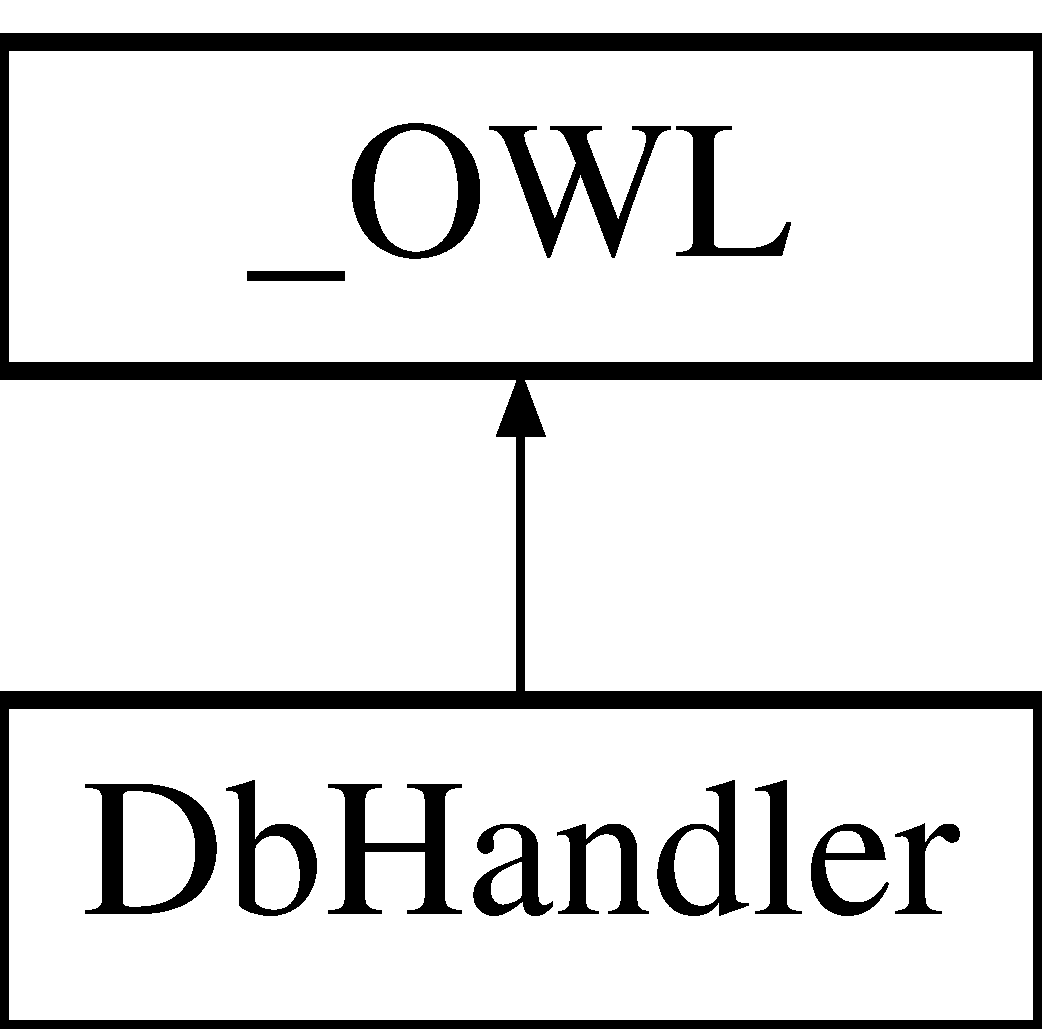
\includegraphics[height=2.000000cm]{classDbHandler}
\end{center}
\end{figure}
\subsection*{Public Member Functions}
\begin{DoxyCompactItemize}
\item 
{\bf \_\-\_\-destruct} ()
\item 
{\bf \_\-\_\-clone} ()
\item 
{\bf alt} (array \$properties)
\item 
{\bf forceReread} ()
\item 
{\bf create} ()
\item 
{\bf isOpen} ()
\item 
{\bf open} ()
\item 
{\bf reset} ()
\item 
{\bf tablename} (\$tablename, \$ignore\_\-backticks=false)
\item 
{\bf setQuery} (\$qry)
\item 
{\bf prepareField} (array \$fielddata)
\item 
{\bf startTransaction} (\$name)
\item 
{\bf commitTransaction} (\$name, \$openNew=false)
\item 
{\bf rollbackTransaction} (\$name, \$openNew=false)
\item 
{\bf resetTable} (\$table)
\item 
{\bf lockTable} (\$tablename, \$locktype)
\item 
{\bf unlockTable} (\$tablename=array())
\item 
{\bf read} (\$flag={\bf DBHANDLE\_\-DATA}, \&\$data, \$quick\_\-query= '', \$line=0, \$file= '[unknown]')
\item 
{\bf tableExists} (\$tablename)
\item 
{\bf escapeString} (\$string)
\item 
{\bf unescapeString} (\$string)
\item 
{\bf prepareRead} (array \$values=array(), array \$tables=array(), array \$searches=array(), array \$joins=array())
\item 
{\bf prepareDelete} (array \$searches=array())
\item 
{\bf prepareUpdate} (array \$values=array(), array \$searches=array(), array \$joins=array())
\item 
{\bf prepareInsert} (array \$values=array())
\item 
{\bf write} (\&\$rows=null, \$line=0, \$file= '[unknown]')
\item 
{\bf lastInsertedId} (\$table=null, \$field=null)
\item 
{\bf close} ()
\item 
{\bf getLastWarning} ()
\item 
{\bf getStatus} ()
\item 
{\bf getSeverity} (\$status=null)
\item 
{\bf succeeded} (\$\_\-ok={\bf OWL\_\-SUCCESS}, \&\$\_\-object=null)
\item 
{\bf signal} (\$level={\bf OWL\_\-INFO}, \&\$text=false)
\item 
{\bf traceback} (\&\$text=false, \$depth=0)
\end{DoxyCompactItemize}
\subsection*{Static Public Member Functions}
\begin{DoxyCompactItemize}
\item 
static {\bf getInstance} ()
\end{DoxyCompactItemize}
\subsection*{Protected Member Functions}
\begin{DoxyCompactItemize}
\item 
{\bf init} ()
\item 
{\bf setCallback} (\$\_\-dispatcher)
\item 
{\bf setCallbackArgument} (array \$\_\-arg)
\item 
{\bf getCallback} ()
\item 
{\bf saveStatus} ()
\item 
{\bf restoreStatus} ()
\item 
{\bf check} (\&\$object, \$level={\bf OWL\_\-WARNING})
\item 
{\bf setStatus} (\$status, \$params=array())
\item 
{\bf setHighSeverity} (\&\$object=null)
\item 
{\bf stackMessage} (\$level={\bf OWL\_\-WARNING})
\end{DoxyCompactItemize}
\subsection*{Protected Attributes}
\begin{DoxyCompactItemize}
\item 
{\bf \$severity}
\end{DoxyCompactItemize}
\subsection*{Private Member Functions}
\begin{DoxyCompactItemize}
\item 
{\bf \_\-\_\-construct} (\$srv= 'localhost', \$db= '', \$usr= '', \$pwd= '', \$dbtype= '{\bf MySQL}')
\item 
{\bf loadDriver} ()
\item 
{\bf connect} ()
\item 
{\bf dbread} (\$qry, \&\$rows, \&\$fields)
\item 
{\bf expandField} (\&\$field, \$check\_\-name=false)
\item 
{\bf tablelist} (array \$tables)
\item 
{\bf whereClause} (array \$searches, array \$joins)
\item 
{\bf updateList} (array \$updates)
\item 
{\bf extractTablelist} (array \$fields)
\item 
{\bf additionalClauses} ()
\end{DoxyCompactItemize}
\subsection*{Private Attributes}
\begin{DoxyCompactItemize}
\item 
{\bf \$id}
\item 
{\bf \$errno}
\item 
{\bf \$error}
\item 
{\bf \$database}
\item 
{\bf \$driver}
\item 
{\bf \$use\_\-backticks}
\item 
{\bf \$rowcount}
\item 
{\bf \$opened}
\item 
{\bf \$db\_\-prefix}
\item 
{\bf \$query}
\item 
{\bf \$ordering}
\item 
{\bf \$grouping}
\item 
{\bf \$having}
\item 
{\bf \$limit}
\item 
{\bf \$query\_\-type}
\item 
{\bf \$transaction}
\item 
{\bf \$locks}
\item 
{\bf \$cloned}
\end{DoxyCompactItemize}
\subsection*{Static Private Attributes}
\begin{DoxyCompactItemize}
\item 
static {\bf \$instance}
\item 
static {\bf \$original\_\-instance}
\end{DoxyCompactItemize}


\subsection{Detailed Description}
Database handler. 

Handler for all database I/O. This singleton class uses an (abstract) class for the actual storage. This class should not be called directly; it is implemented by class \doxyref{DataHandler}{p.}{classDataHandler} \begin{DoxyAuthor}{Author}
Oscar van Eijk, Oveas Functionality Provider 
\end{DoxyAuthor}
\begin{Desc}
\item[{\bf Todo}]Implement retries using the isRetryable() driver method, a max\_\-retries and a max\_\-retry\_\-wait config settings \end{Desc}
\begin{DoxyVersion}{Version}
May 15, 2007 -\/-\/ O van Eijk -\/-\/ initial version for Terra-\/Terra 

Jul 29, 2008 -\/-\/ O van Eijk -\/-\/ Modified version for \doxyref{OWL}{p.}{classOWL} 
\end{DoxyVersion}


\subsection{Constructor \& Destructor Documentation}
\index{DbHandler@{DbHandler}!\_\-\_\-construct@{\_\-\_\-construct}}
\index{\_\-\_\-construct@{\_\-\_\-construct}!DbHandler@{DbHandler}}
\subsubsection[{\_\-\_\-construct}]{\setlength{\rightskip}{0pt plus 5cm}DbHandler::\_\-\_\-construct (
\begin{DoxyParamCaption}
\item[{\$}]{srv = {\ttfamily 'localhost'}, }
\item[{\$}]{db = {\ttfamily ''}, }
\item[{\$}]{usr = {\ttfamily ''}, }
\item[{\$}]{pwd = {\ttfamily ''}, }
\item[{\$}]{dbtype = {\ttfamily '{\bf MySQL}'}}
\end{DoxyParamCaption}
)\hspace{0.3cm}{\ttfamily  [private]}}\label{classDbHandler_ae54e9d4643f41a9296167086f6a769fc}
Class constructor; opens the database connection. 
\begin{DoxyParams}[1]{Parameters}
\mbox{\tt in}  & {\em \$srv} & Database server \\
\hline
\mbox{\tt in}  & {\em \$db} & Database name \\
\hline
\mbox{\tt in}  & {\em \$usr} & Username to connect with \\
\hline
\mbox{\tt in}  & {\em \$pwd} & Password to use for connection \\
\hline
\mbox{\tt in}  & {\em \$dbtype} & Database type, used to load the driver \\
\hline
\end{DoxyParams}
\begin{DoxyAuthor}{Author}
Oscar van Eijk, Oveas Functionality Provider 
\end{DoxyAuthor}


References ConfigHandler::get(), \_\-OWL::init(), loadDriver(), and \_\-OWL::setStatus().

\index{DbHandler@{DbHandler}!\_\-\_\-destruct@{\_\-\_\-destruct}}
\index{\_\-\_\-destruct@{\_\-\_\-destruct}!DbHandler@{DbHandler}}
\subsubsection[{\_\-\_\-destruct}]{\setlength{\rightskip}{0pt plus 5cm}DbHandler::\_\-\_\-destruct (
\begin{DoxyParamCaption}
{}
\end{DoxyParamCaption}
)}\label{classDbHandler_a7cd6bd727d1f296eb5dbfae6ca36ab3f}
Class destructor; closes the database connection \begin{DoxyAuthor}{Author}
Oscar van Eijk, Oveas Functionality Provider 
\end{DoxyAuthor}


Reimplemented from {\bf \_\-OWL} \doxyref{}{p.}{class__OWL_a44fd2222476a3109286cc82d92b6bbcc}.



References close(), commitTransaction(), ConfigHandler::get(), rollbackTransaction(), and unlockTable().



\subsection{Member Function Documentation}
\index{DbHandler@{DbHandler}!\_\-\_\-clone@{\_\-\_\-clone}}
\index{\_\-\_\-clone@{\_\-\_\-clone}!DbHandler@{DbHandler}}
\subsubsection[{\_\-\_\-clone}]{\setlength{\rightskip}{0pt plus 5cm}DbHandler::\_\-\_\-clone (
\begin{DoxyParamCaption}
{}
\end{DoxyParamCaption}
)}\label{classDbHandler_ada20e62b915bc87a1de28389a2ee81e1}
Implementation of the \doxyref{\_\-\_\-clone()}{p.}{classDbHandler_ada20e62b915bc87a1de28389a2ee81e1} function. The current connection will be closed, and a property will be set to indicate this is a cloned object. After that, the \doxyref{alt()}{p.}{classDbHandler_ac3a8e0bfe2491e17bc527715505f90a7} method can be used to change connection info. \begin{DoxyAuthor}{Author}
Oscar van Eijk, Oveas Functionality Provider 
\end{DoxyAuthor}


References \$instance, close(), reset(), and \_\-OWL::setStatus().

\index{DbHandler@{DbHandler}!additionalClauses@{additionalClauses}}
\index{additionalClauses@{additionalClauses}!DbHandler@{DbHandler}}
\subsubsection[{additionalClauses}]{\setlength{\rightskip}{0pt plus 5cm}DbHandler::additionalClauses (
\begin{DoxyParamCaption}
{}
\end{DoxyParamCaption}
)\hspace{0.3cm}{\ttfamily  [private]}}\label{classDbHandler_a9380a7c5c11003d51addd9ea02d41f89}
Check if additional clauses (like GROUP BY, ORDER BY etc) have been defined, and compose this depending on the query type. \begin{DoxyReturn}{Returns}
String with additional clauses 
\end{DoxyReturn}
\begin{DoxyAuthor}{Author}
Oscar van Eijk, Oveas Functionality Provider 
\end{DoxyAuthor}


References expandField().



Referenced by prepareDelete(), prepareInsert(), prepareRead(), and prepareUpdate().

\index{DbHandler@{DbHandler}!alt@{alt}}
\index{alt@{alt}!DbHandler@{DbHandler}}
\subsubsection[{alt}]{\setlength{\rightskip}{0pt plus 5cm}DbHandler::alt (
\begin{DoxyParamCaption}
\item[{array \$}]{properties}
\end{DoxyParamCaption}
)}\label{classDbHandler_ac3a8e0bfe2491e17bc527715505f90a7}
On a cloned database object, set an alternative, prefix or connection. 
\begin{DoxyParams}[1]{Parameters}
\mbox{\tt in}  & {\em \$properties} & An indexed array with the properties that should be changed. Supported are:
\begin{DoxyItemize}
\item prefix : The table prefix
\item server : Database server
\item name : Database name
\item username : Username to connect with
\item password : Password to use for connection
\item dbdriver : Database type (reserved for future use, currently only \doxyref{MySQL}{p.}{classMySQL} is implemented) 
\end{DoxyItemize}\\
\hline
\end{DoxyParams}
\begin{DoxyAuthor}{Author}
Oscar van Eijk, Oveas Functionality Provider 
\end{DoxyAuthor}


References loadDriver(), open(), and \_\-OWL::setStatus().

\index{DbHandler@{DbHandler}!check@{check}}
\index{check@{check}!DbHandler@{DbHandler}}
\subsubsection[{check}]{\setlength{\rightskip}{0pt plus 5cm}\_\-OWL::check (
\begin{DoxyParamCaption}
\item[{\&\$}]{object, }
\item[{\$}]{level = {\ttfamily {\bf OWL\_\-WARNING}}}
\end{DoxyParamCaption}
)\hspace{0.3cm}{\ttfamily  [protected, inherited]}}\label{class__OWL_ae2e3c56e5f3c4ce4156c6b1bb1c50f63}
This is a helper function for lazy developers. Some checks have to be made quite often, this is a kinda macro to handle that. It compares the own severity level with that of a given object. If the highest level is above a given max, a traceback and reset are performed.


\begin{DoxyParams}[1]{Parameters}
\mbox{\tt in}  & {\em \$object} & Pointer to an object to check against \\
\hline
\mbox{\tt in}  & {\em \$level} & The maximum severity level \\
\hline
\end{DoxyParams}
\begin{DoxyReturn}{Returns}
True if the severity level was correct (below the max), otherwise false 
\end{DoxyReturn}
\begin{DoxyAuthor}{Author}
Oscar van Eijk, Oveas Functionality Provider 
\end{DoxyAuthor}


References \_\-OWL::reset(), \_\-OWL::setHighSeverity(), and \_\-OWL::traceback().



Referenced by SessionHandler::write().

\index{DbHandler@{DbHandler}!close@{close}}
\index{close@{close}!DbHandler@{DbHandler}}
\subsubsection[{close}]{\setlength{\rightskip}{0pt plus 5cm}DbHandler::close (
\begin{DoxyParamCaption}
{}
\end{DoxyParamCaption}
)}\label{classDbHandler_ad3d2853bbd2d1962710907e34afb424f}
Close the database and disconnect from the server. This function is called on program shutdown. Although the database will be closed already by PHP, this function might be called at any time manually; is also updates the 'opened' variable. \begin{DoxyAuthor}{Author}
Oscar van Eijk, Oveas Functionality Provider 
\end{DoxyAuthor}


Referenced by \_\-\_\-clone(), \_\-\_\-destruct(), create(), and forceReread().

\index{DbHandler@{DbHandler}!commitTransaction@{commitTransaction}}
\index{commitTransaction@{commitTransaction}!DbHandler@{DbHandler}}
\subsubsection[{commitTransaction}]{\setlength{\rightskip}{0pt plus 5cm}DbHandler::commitTransaction (
\begin{DoxyParamCaption}
\item[{\$}]{name, }
\item[{\$}]{openNew = {\ttfamily false}}
\end{DoxyParamCaption}
)}\label{classDbHandler_ae31ec569a60f730fb1de2ac2b1265338}
Commit database transaction 
\begin{DoxyParams}[1]{Parameters}
\mbox{\tt in}  & {\em \$name} & Transaction name (reserverd for future use) \\
\hline
\mbox{\tt in}  & {\em \$openNew} & Boolean set to true when a new transaction must be opened immediately \\
\hline
\end{DoxyParams}
\begin{DoxyReturn}{Returns}
Object severity status 
\end{DoxyReturn}
\begin{DoxyAuthor}{Author}
Oscar van Eijk, Oveas Functionality Provider 
\end{DoxyAuthor}


References \_\-OWL::setStatus().



Referenced by \_\-\_\-destruct().

\index{DbHandler@{DbHandler}!connect@{connect}}
\index{connect@{connect}!DbHandler@{DbHandler}}
\subsubsection[{connect}]{\setlength{\rightskip}{0pt plus 5cm}DbHandler::connect (
\begin{DoxyParamCaption}
{}
\end{DoxyParamCaption}
)\hspace{0.3cm}{\ttfamily  [private]}}\label{classDbHandler_a9cf52ba614981a0082063d57290d3b7c}
Connect to the database server \begin{DoxyReturn}{Returns}
True on success, otherwise False 
\end{DoxyReturn}
\begin{DoxyAuthor}{Author}
Oscar van Eijk, Oveas Functionality Provider 
\end{DoxyAuthor}


References ConfigHandler::get(), and \_\-OWL::setStatus().



Referenced by create(), and open().

\index{DbHandler@{DbHandler}!create@{create}}
\index{create@{create}!DbHandler@{DbHandler}}
\subsubsection[{create}]{\setlength{\rightskip}{0pt plus 5cm}DbHandler::create (
\begin{DoxyParamCaption}
{}
\end{DoxyParamCaption}
)}\label{classDbHandler_ac9e93cb0ab57f03b2719eebd0c0ee2ef}
Create a new database \begin{DoxyReturn}{Returns}
Severity level 
\end{DoxyReturn}
\begin{DoxyAuthor}{Author}
Oscar van Eijk, Oveas Functionality Provider 
\end{DoxyAuthor}


References close(), connect(), and \_\-OWL::setStatus().

\index{DbHandler@{DbHandler}!dbread@{dbread}}
\index{dbread@{dbread}!DbHandler@{DbHandler}}
\subsubsection[{dbread}]{\setlength{\rightskip}{0pt plus 5cm}DbHandler::dbread (
\begin{DoxyParamCaption}
\item[{\$}]{qry, }
\item[{\&\$}]{rows, }
\item[{\&\$}]{fields}
\end{DoxyParamCaption}
)\hspace{0.3cm}{\ttfamily  [private]}}\label{classDbHandler_a130e49aa639fecb46ce6719ddcb0d72f}
Read from the database. 
\begin{DoxyParams}[1]{Parameters}
\mbox{\tt in}  & {\em \$qry} & Database query string. \\
\hline
\mbox{\tt out}  & {\em \$rows} & Number of rows matched \\
\hline
\mbox{\tt out}  & {\em \$fields} & Number of fields per row \\
\hline
\end{DoxyParams}
\begin{DoxyReturn}{Returns}
A 2D array with all data, or false on failures 
\end{DoxyReturn}
\begin{DoxyAuthor}{Author}
Oscar van Eijk, Oveas Functionality Provider 
\end{DoxyAuthor}


References OWLdbg\_\-add(), and \_\-OWL::setStatus().



Referenced by read().

\index{DbHandler@{DbHandler}!escapeString@{escapeString}}
\index{escapeString@{escapeString}!DbHandler@{DbHandler}}
\subsubsection[{escapeString}]{\setlength{\rightskip}{0pt plus 5cm}DbHandler::escapeString (
\begin{DoxyParamCaption}
\item[{\$}]{string}
\end{DoxyParamCaption}
)}\label{classDbHandler_a84d876a07a292f4a7bd49e5acfac9d14}
Call the current DBtype's escape function for character strings. 
\begin{DoxyParams}{Parameters}
{\em \$string} & The string that should be escaped \\
\hline
\end{DoxyParams}
\begin{DoxyReturn}{Returns}
The escaped string 
\end{DoxyReturn}
\begin{DoxyAuthor}{Author}
Oscar van Eijk, Oveas Functionality Provider 
\end{DoxyAuthor}
\index{DbHandler@{DbHandler}!expandField@{expandField}}
\index{expandField@{expandField}!DbHandler@{DbHandler}}
\subsubsection[{expandField}]{\setlength{\rightskip}{0pt plus 5cm}DbHandler::expandField (
\begin{DoxyParamCaption}
\item[{\&\$}]{field, }
\item[{\$}]{check\_\-name = {\ttfamily false}}
\end{DoxyParamCaption}
)\hspace{0.3cm}{\ttfamily  [private]}}\label{classDbHandler_ad8dac71adf4d540270b5b2c87da114a8}
Change a fieldname in the format 'table\#field' to the format '`[prefix]table.field`' The fieldname can have additional \#-\/seperated elements, which contain the method from the database driver and its arguments (that will be passed as an array) 
\begin{DoxyParams}[1]{Parameters}
\mbox{\tt in,out}  & {\em \$field} & Fieldname to expand \\
\hline
\mbox{\tt in}  & {\em \$check\_\-name} & Boolean which is true if the fieldname should be returned with 'AS'. Default is false \\
\hline
\end{DoxyParams}
\begin{DoxyAuthor}{Author}
Oscar van Eijk, Oveas Functionality Provider 
\end{DoxyAuthor}


References tablename().



Referenced by additionalClauses(), prepareInsert(), prepareRead(), updateList(), and whereClause().

\index{DbHandler@{DbHandler}!extractTablelist@{extractTablelist}}
\index{extractTablelist@{extractTablelist}!DbHandler@{DbHandler}}
\subsubsection[{extractTablelist}]{\setlength{\rightskip}{0pt plus 5cm}DbHandler::extractTablelist (
\begin{DoxyParamCaption}
\item[{array \$}]{fields}
\end{DoxyParamCaption}
)\hspace{0.3cm}{\ttfamily  [private]}}\label{classDbHandler_ab900537e8f8170436f2be39e2a9026cf}
Create an array with unique tablenames as extracted from an array of fields in the format (table::field =$>$ value, ...) 
\begin{DoxyParams}[1]{Parameters}
\mbox{\tt in}  & {\em \$fields} & An array with fields \\
\hline
\end{DoxyParams}
\begin{DoxyReturn}{Returns}
Array with tablenames 
\end{DoxyReturn}
\begin{DoxyAuthor}{Author}
Oscar van Eijk, Oveas Functionality Provider 
\end{DoxyAuthor}


Referenced by prepareDelete(), prepareInsert(), and prepareUpdate().

\index{DbHandler@{DbHandler}!forceReread@{forceReread}}
\index{forceReread@{forceReread}!DbHandler@{DbHandler}}
\subsubsection[{forceReread}]{\setlength{\rightskip}{0pt plus 5cm}DbHandler::forceReread (
\begin{DoxyParamCaption}
{}
\end{DoxyParamCaption}
)}\label{classDbHandler_a1a342f747e4e4c10c00d7d6066d50d59}
Hmmm.... we need this method as the result of a race condition (sort of... I think...); if an alternative database (clone) is opened first, that's the default connection, which is probably the case in most situation since the owl config table is read early in the init phase. I need to think about it... is this solution acceptable? So we need something smarter here? This method is allowed to be called only once by OWLLoader; maybe some checks? \begin{DoxyAuthor}{Author}
Oscar van Eijk, Oveas Functionality Provider 
\end{DoxyAuthor}


References close(), ConfigHandler::get(), loadDriver(), and open().

\index{DbHandler@{DbHandler}!getCallback@{getCallback}}
\index{getCallback@{getCallback}!DbHandler@{DbHandler}}
\subsubsection[{getCallback}]{\setlength{\rightskip}{0pt plus 5cm}\_\-OWL::getCallback (
\begin{DoxyParamCaption}
{}
\end{DoxyParamCaption}
)\hspace{0.3cm}{\ttfamily  [protected, inherited]}}\label{class__OWL_acb46ff88f43ca66f1268d3f5199c3f8d}
Retrieve a previously set (callback) dispatcher. The (callback) dispatcher is cleared immediatly. \begin{DoxyReturn}{Returns}
The dispatcher, of null on failure. 
\end{DoxyReturn}
\begin{DoxyAuthor}{Author}
Oscar van Eijk, Oveas Functionality Provider 
\end{DoxyAuthor}


Reimplemented in {\bf Dispatcher} \doxyref{}{p.}{classDispatcher_a31c4bd4e4eaee7ef90b1ea364a901447}.



References OWL::factory().

\index{DbHandler@{DbHandler}!getInstance@{getInstance}}
\index{getInstance@{getInstance}!DbHandler@{DbHandler}}
\subsubsection[{getInstance}]{\setlength{\rightskip}{0pt plus 5cm}static DbHandler::getInstance (
\begin{DoxyParamCaption}
{}
\end{DoxyParamCaption}
)\hspace{0.3cm}{\ttfamily  [static]}}\label{classDbHandler_a72b64ea1342d97d300d564a7641627d7}
Return a reference to my implementation. If necessary, create that implementation first. \begin{DoxyReturn}{Returns}
Object instance ID 
\end{DoxyReturn}
\begin{DoxyAuthor}{Author}
Oscar van Eijk, Oveas Functionality Provider 
\end{DoxyAuthor}


References \$instance, \$original\_\-instance, and ConfigHandler::get().

\index{DbHandler@{DbHandler}!getLastWarning@{getLastWarning}}
\index{getLastWarning@{getLastWarning}!DbHandler@{DbHandler}}
\subsubsection[{getLastWarning}]{\setlength{\rightskip}{0pt plus 5cm}\_\-OWL::getLastWarning (
\begin{DoxyParamCaption}
{}
\end{DoxyParamCaption}
)\hspace{0.3cm}{\ttfamily  [inherited]}}\label{class__OWL_a1888f52fc2d0ec29e146925ccad70a6b}
Get the last warning or error message. \begin{DoxyReturn}{Returns}
null if there was no error (severity below OWL\_\-WARNING), otherwise the error text. 
\end{DoxyReturn}
\begin{DoxyAuthor}{Author}
Oscar van Eijk, Oveas Functionality Provider 
\end{DoxyAuthor}


References \_\-OWL::signal().

\index{DbHandler@{DbHandler}!getSeverity@{getSeverity}}
\index{getSeverity@{getSeverity}!DbHandler@{DbHandler}}
\subsubsection[{getSeverity}]{\setlength{\rightskip}{0pt plus 5cm}\_\-OWL::getSeverity (
\begin{DoxyParamCaption}
\item[{\$}]{status = {\ttfamily null}}
\end{DoxyParamCaption}
)\hspace{0.3cm}{\ttfamily  [inherited]}}\label{class__OWL_a2374613f9bb7eccf49a5dbc9a9ef4751}
Get the current object severity level. 
\begin{DoxyParams}[1]{Parameters}
\mbox{\tt in}  & {\em \$status} & An optional parameter to check an other status code i.s.o the object's current status. \\
\hline
\end{DoxyParams}
\begin{DoxyReturn}{Returns}
Status severity level 
\end{DoxyReturn}
\begin{DoxyAuthor}{Author}
Oscar van Eijk, Oveas Functionality Provider 
\end{DoxyAuthor}


References \_\-OWL::\$status.



Referenced by LogHandler::composeMessage(), LogHandler::log(), and DataHandler::setKey().

\index{DbHandler@{DbHandler}!getStatus@{getStatus}}
\index{getStatus@{getStatus}!DbHandler@{DbHandler}}
\subsubsection[{getStatus}]{\setlength{\rightskip}{0pt plus 5cm}\_\-OWL::getStatus (
\begin{DoxyParamCaption}
{}
\end{DoxyParamCaption}
)\hspace{0.3cm}{\ttfamily  [final, inherited]}}\label{class__OWL_ac1f1643ff5b5db7c326c30477603358d}
Get the current object status. \begin{DoxyReturn}{Returns}
Object's status code 
\end{DoxyReturn}
\begin{DoxyAuthor}{Author}
Oscar van Eijk, Oveas Functionality Provider 
\end{DoxyAuthor}


Referenced by SchemeHandler::compare().

\index{DbHandler@{DbHandler}!init@{init}}
\index{init@{init}!DbHandler@{DbHandler}}
\subsubsection[{init}]{\setlength{\rightskip}{0pt plus 5cm}\_\-OWL::init (
\begin{DoxyParamCaption}
{}
\end{DoxyParamCaption}
)\hspace{0.3cm}{\ttfamily  [protected, inherited]}}\label{class__OWL_ae0ef3ded56e8a6b34b6461e5a721cd3e}
This function should be called by all constuctors. It initializes the general characteristics. Status is 'warning' by default, it's up to the contructor to set a proper status; if it's still 'warning', this $\ast$might$\ast$ indicate something went wrong. \begin{DoxyAuthor}{Author}
Oscar van Eijk, Oveas Functionality Provider 
\end{DoxyAuthor}


References OWL::factory(), and \_\-OWL::setStatus().



Referenced by FormFieldPlugin::\_\-\_\-construct(), Document::\_\-\_\-construct(), ContainerPlugin::\_\-\_\-construct(), Container::\_\-\_\-construct(), SocketHandler::\_\-\_\-construct(), SessionHandler::\_\-\_\-construct(), SchemeHandler::\_\-\_\-construct(), LogHandler::\_\-\_\-construct(), ImageHandler::\_\-\_\-construct(), FormHandler::\_\-\_\-construct(), FileHandler::\_\-\_\-construct(), \_\-\_\-construct(), HDataHandler::\_\-\_\-construct(), DataHandler::\_\-\_\-construct(), OWL::\_\-\_\-construct(), Mail::\_\-\_\-construct(), Group::\_\-\_\-construct(), Form::\_\-\_\-construct(), Dispatcher::\_\-\_\-construct(), and User::construct().

\index{DbHandler@{DbHandler}!isOpen@{isOpen}}
\index{isOpen@{isOpen}!DbHandler@{DbHandler}}
\subsubsection[{isOpen}]{\setlength{\rightskip}{0pt plus 5cm}DbHandler::isOpen (
\begin{DoxyParamCaption}
{}
\end{DoxyParamCaption}
)}\label{classDbHandler_a71b713d7b974200e64bd606e3b099c38}
Let other objects check if th database connection is opened \begin{DoxyReturn}{Returns}
boolean, True when opened 
\end{DoxyReturn}
\begin{DoxyAuthor}{Author}
Oscar van Eijk, Oveas Functionality Provider 
\end{DoxyAuthor}
\index{DbHandler@{DbHandler}!lastInsertedId@{lastInsertedId}}
\index{lastInsertedId@{lastInsertedId}!DbHandler@{DbHandler}}
\subsubsection[{lastInsertedId}]{\setlength{\rightskip}{0pt plus 5cm}DbHandler::lastInsertedId (
\begin{DoxyParamCaption}
\item[{\$}]{table = {\ttfamily null}, }
\item[{\$}]{field = {\ttfamily null}}
\end{DoxyParamCaption}
)}\label{classDbHandler_a8e1ac478bf6f4e2285d13141fd75bb9e}
Return the last ID after a newly inserted record holding an AUTO\_\-INCREMENT field 
\begin{DoxyParams}[1]{Parameters}
\mbox{\tt in}  & {\em \$table} & Table name holding the auto increment field \\
\hline
\mbox{\tt in}  & {\em \$field} & Name of the auto increment field \\
\hline
\end{DoxyParams}
\begin{DoxyReturn}{Returns}
The number that was last inserted 
\end{DoxyReturn}
\begin{DoxyAuthor}{Author}
Oscar van Eijk, Oveas Functionality Provider 
\end{DoxyAuthor}
\index{DbHandler@{DbHandler}!loadDriver@{loadDriver}}
\index{loadDriver@{loadDriver}!DbHandler@{DbHandler}}
\subsubsection[{loadDriver}]{\setlength{\rightskip}{0pt plus 5cm}DbHandler::loadDriver (
\begin{DoxyParamCaption}
{}
\end{DoxyParamCaption}
)\hspace{0.3cm}{\ttfamily  [private]}}\label{classDbHandler_ab4db7c4fa445700b96a2d4b1be6e50a4}
Create a new instance of the database driver \begin{DoxyAuthor}{Author}
Oscar van Eijk, Oveas Functionality Provider 
\end{DoxyAuthor}


References OWLloader::getDriver(), and toBool().



Referenced by \_\-\_\-construct(), alt(), and forceReread().

\index{DbHandler@{DbHandler}!lockTable@{lockTable}}
\index{lockTable@{lockTable}!DbHandler@{DbHandler}}
\subsubsection[{lockTable}]{\setlength{\rightskip}{0pt plus 5cm}DbHandler::lockTable (
\begin{DoxyParamCaption}
\item[{\$}]{tablename, }
\item[{\$}]{locktype}
\end{DoxyParamCaption}
)}\label{classDbHandler_a27c45a702ae53310ccc159a88bc4234f}
Lock one or more tables 
\begin{DoxyParams}[1]{Parameters}
\mbox{\tt in}  & {\em \$tablename} & Tablename or array of tables \\
\hline
\mbox{\tt in}  & {\em \$locktype} & Locktype as defined in \doxyref{Table lock type}{p.}{group__DBDRIVER__TableLock} \\
\hline
\end{DoxyParams}
\begin{DoxyReturn}{Returns}
Object severity status 
\end{DoxyReturn}
\begin{DoxyAuthor}{Author}
Oscar van Eijk, Oveas Functionality Provider 
\end{DoxyAuthor}
\begin{DoxyNote}{Note}
In \doxyref{MySQL}{p.}{classMySQL}, locks will be released implicetly when a new lock is requested. Also when a new transaction is started, all existing locks are released, so when table locking is required within a transaction, always call \doxyref{lockTable()}{p.}{classDbHandler_a27c45a702ae53310ccc159a88bc4234f} {\itshape after\/} \doxyref{startTransaction()}{p.}{classDbHandler_a19f0cb54f362ab3f919cfc2b940800c0} 
\end{DoxyNote}
\begin{Desc}
\item[{\bf Todo}]This method currenly supports only 1 table and no aliases, must be changed! \end{Desc}


References ConfigHandler::get(), and \_\-OWL::setStatus().

\index{DbHandler@{DbHandler}!open@{open}}
\index{open@{open}!DbHandler@{DbHandler}}
\subsubsection[{open}]{\setlength{\rightskip}{0pt plus 5cm}DbHandler::open (
\begin{DoxyParamCaption}
{}
\end{DoxyParamCaption}
)}\label{classDbHandler_afccbfc69ead84f8445116e050d1cfc2d}
Opens the database connection. \begin{DoxyReturn}{Returns}
Severity level 
\end{DoxyReturn}
\begin{DoxyAuthor}{Author}
Oscar van Eijk, Oveas Functionality Provider 
\end{DoxyAuthor}


References connect(), and \_\-OWL::setStatus().



Referenced by alt(), forceReread(), and read().

\index{DbHandler@{DbHandler}!prepareDelete@{prepareDelete}}
\index{prepareDelete@{prepareDelete}!DbHandler@{DbHandler}}
\subsubsection[{prepareDelete}]{\setlength{\rightskip}{0pt plus 5cm}DbHandler::prepareDelete (
\begin{DoxyParamCaption}
\item[{array \$}]{searches = {\ttfamily array()}}
\end{DoxyParamCaption}
)}\label{classDbHandler_a4dce3c43b43a82a1ac0e3ba2c83309ee}
Prepare a delete query. Data is taken from the arrays that are passed to this function. All fieldnames are in the format 'table\#field', where the table is not yet prefixed. 
\begin{DoxyParams}[1]{Parameters}
\mbox{\tt in}  & {\em \$searches} & Given values that have to match \\
\hline
\end{DoxyParams}
\begin{DoxyReturn}{Returns}
Severity level 
\end{DoxyReturn}
\begin{DoxyAuthor}{Author}
Oscar van Eijk, Oveas Functionality Provider 
\end{DoxyAuthor}


References additionalClauses(), extractTablelist(), OWLdbg\_\-add(), \_\-OWL::setStatus(), tablelist(), and whereClause().

\index{DbHandler@{DbHandler}!prepareField@{prepareField}}
\index{prepareField@{prepareField}!DbHandler@{DbHandler}}
\subsubsection[{prepareField}]{\setlength{\rightskip}{0pt plus 5cm}DbHandler::prepareField (
\begin{DoxyParamCaption}
\item[{array \$}]{fielddata}
\end{DoxyParamCaption}
)}\label{classDbHandler_aab87f0d23357d708c7f327e3875366ad}
Prepare a field for use in the upconimg query using the array as set by DbHandler::set(). Internal arrays are filled with grouping data, ordering data etc. if required., 
\begin{DoxyParams}[1]{Parameters}
\mbox{\tt in}  & {\em \$fielddata} & Array with a description of the field, \\
\hline
\end{DoxyParams}
\begin{DoxySeeAlso}{See also}
DbHandler::set() 
\end{DoxySeeAlso}
\begin{DoxyReturn}{Returns}
An array with two elements: the fieldname in the format that will be handled by \doxyref{DbHandler::expandField()}{p.}{classDbHandler_ad8dac71adf4d540270b5b2c87da114a8}, and the value which might be a normal value, an array of values of a value as set by a driver function (using database functions). On errors, null is returned. 
\end{DoxyReturn}
\begin{DoxyAuthor}{Author}
Oscar van Eijk, Oveas Functionality Provider 
\end{DoxyAuthor}


References \_\-OWL::setStatus().

\index{DbHandler@{DbHandler}!prepareInsert@{prepareInsert}}
\index{prepareInsert@{prepareInsert}!DbHandler@{DbHandler}}
\subsubsection[{prepareInsert}]{\setlength{\rightskip}{0pt plus 5cm}DbHandler::prepareInsert (
\begin{DoxyParamCaption}
\item[{array \$}]{values = {\ttfamily array()}}
\end{DoxyParamCaption}
)}\label{classDbHandler_a50f426084a888714b72bedb42de7ebc4}
Prepare an insert query. Data is taken from the arrays that are passed to this function. All fieldnames are in the format 'table\#field', where the table is not yet prefixed. 
\begin{DoxyParams}[1]{Parameters}
\mbox{\tt in}  & {\em \$values} & Given database values \\
\hline
\end{DoxyParams}
\begin{DoxyReturn}{Returns}
Severity level 
\end{DoxyReturn}
\begin{DoxyAuthor}{Author}
Oscar van Eijk, Oveas Functionality Provider 
\end{DoxyAuthor}


References additionalClauses(), expandField(), extractTablelist(), OWLdbg\_\-add(), \_\-OWL::setStatus(), and tablename().

\index{DbHandler@{DbHandler}!prepareRead@{prepareRead}}
\index{prepareRead@{prepareRead}!DbHandler@{DbHandler}}
\subsubsection[{prepareRead}]{\setlength{\rightskip}{0pt plus 5cm}DbHandler::prepareRead (
\begin{DoxyParamCaption}
\item[{array \$}]{values = {\ttfamily array()}, }
\item[{array \$}]{tables = {\ttfamily array()}, }
\item[{array \$}]{searches = {\ttfamily array()}, }
\item[{array \$}]{joins = {\ttfamily array()}}
\end{DoxyParamCaption}
)}\label{classDbHandler_a2f749a426fa9dbfe1b58a7d0d4263d1f}
Prepare a read query. Data is taken from the arrays that are passed to this function. All fieldnames are in the format 'table\#field', where the table is not yet prefixed. 
\begin{DoxyParams}[1]{Parameters}
\mbox{\tt in}  & {\em \$values} & Values that will be read \\
\hline
\mbox{\tt in}  & {\em \$tables} & Tables from which will be read \\
\hline
\mbox{\tt in}  & {\em \$searches} & Given values that have to match \\
\hline
\mbox{\tt in}  & {\em \$joins} & Joins on the given tables \\
\hline
\end{DoxyParams}
\begin{DoxyReturn}{Returns}
Severity level 
\end{DoxyReturn}
\begin{DoxyAuthor}{Author}
Oscar van Eijk, Oveas Functionality Provider 
\end{DoxyAuthor}


References additionalClauses(), expandField(), OWLdbg\_\-add(), \_\-OWL::setStatus(), tablelist(), and whereClause().

\index{DbHandler@{DbHandler}!prepareUpdate@{prepareUpdate}}
\index{prepareUpdate@{prepareUpdate}!DbHandler@{DbHandler}}
\subsubsection[{prepareUpdate}]{\setlength{\rightskip}{0pt plus 5cm}DbHandler::prepareUpdate (
\begin{DoxyParamCaption}
\item[{array \$}]{values = {\ttfamily array()}, }
\item[{array \$}]{searches = {\ttfamily array()}, }
\item[{array \$}]{joins = {\ttfamily array()}}
\end{DoxyParamCaption}
)}\label{classDbHandler_abe6db4c3099ca5cfcfb75e9eb34ba2af}
Prepare an update query. Data is taken from the arrays that are passed to this function. All fieldnames are in the format 'table\#field', where the table is not yet prefixed. 
\begin{DoxyParams}[1]{Parameters}
\mbox{\tt in}  & {\em \$values} & Given database values \\
\hline
\mbox{\tt in}  & {\em \$searches} & List of fieldnames that will be used in the where clause. All fields not in this array will be updated! \\
\hline
\mbox{\tt in}  & {\em \$joins} & Joins on the given tables \\
\hline
\end{DoxyParams}
\begin{DoxyReturn}{Returns}
Severity level 
\end{DoxyReturn}
\begin{DoxyAuthor}{Author}
Oscar van Eijk, Oveas Functionality Provider 
\end{DoxyAuthor}


References additionalClauses(), extractTablelist(), OWLdbg\_\-add(), \_\-OWL::setStatus(), tablelist(), updateList(), and whereClause().

\index{DbHandler@{DbHandler}!read@{read}}
\index{read@{read}!DbHandler@{DbHandler}}
\subsubsection[{read}]{\setlength{\rightskip}{0pt plus 5cm}DbHandler::read (
\begin{DoxyParamCaption}
\item[{\$}]{flag = {\ttfamily {\bf DBHANDLE\_\-DATA}}, }
\item[{\&\$}]{data, }
\item[{\$}]{quick\_\-query = {\ttfamily ''}, }
\item[{\$}]{line = {\ttfamily 0}, }
\item[{\$}]{file = {\ttfamily '[unknown]'}}
\end{DoxyParamCaption}
)}\label{classDbHandler_a5ebfdc2acfcb0e9cbc2861fc55c7127c}
Read from the database. The return value depends on the flag. By default, the selected rows(s) are returned in a 2d array. 
\begin{DoxyParams}[1]{Parameters}
\mbox{\tt in}  & {\em \$flag} & Flag that identifies how data should be returned; as data (default) or the number of rows \\
\hline
\mbox{\tt out}  & {\em \$data} & The retrieved value in a format depending on the flag:
\begin{DoxyItemize}
\item DBHANDLE\_\-ROWCOUNT; Number of matching rows
\item DBHANDLE\_\-FIELDCOUNT; Number of fields per rows
\item DBHANDLE\_\-TOTALFIELDCOUNT; Total number op fields
\item DBHANDLE\_\-DATA (default); A 2D array with all data
\item DBHANDLE\_\-SINGLEROW; The first matching row in a 1D array
\item DBHANDLE\_\-SINGLEFIELD; The first matching field 
\end{DoxyItemize}\\
\hline
\mbox{\tt in}  & {\em \$quick\_\-query} & Database query string. If empty, \$this-\/$>$query is used \\
\hline
\mbox{\tt in}  & {\em \$line} & Line number of this call \\
\hline
\mbox{\tt in}  & {\em \$file} & File that made the call to this method \\
\hline
\end{DoxyParams}
\begin{DoxyReturn}{Returns}
Severity level 
\end{DoxyReturn}
\begin{DoxyAuthor}{Author}
Oscar van Eijk, Oveas Functionality Provider 
\end{DoxyAuthor}


References dbread(), open(), and \_\-OWL::setStatus().

\index{DbHandler@{DbHandler}!reset@{reset}}
\index{reset@{reset}!DbHandler@{DbHandler}}
\subsubsection[{reset}]{\setlength{\rightskip}{0pt plus 5cm}DbHandler::reset (
\begin{DoxyParamCaption}
{}
\end{DoxyParamCaption}
)}\label{classDbHandler_a9982df4830f05803935bb31bac7fae3d}
Reset the object \begin{DoxyAuthor}{Author}
Oscar van Eijk, Oveas Functionality Provider 
\end{DoxyAuthor}


Reimplemented from {\bf \_\-OWL} \doxyref{}{p.}{class__OWL_a2f2a042bcf31965194c03033df0edc9b}.



Referenced by \_\-\_\-clone().

\index{DbHandler@{DbHandler}!resetTable@{resetTable}}
\index{resetTable@{resetTable}!DbHandler@{DbHandler}}
\subsubsection[{resetTable}]{\setlength{\rightskip}{0pt plus 5cm}DbHandler::resetTable (
\begin{DoxyParamCaption}
\item[{\$}]{table}
\end{DoxyParamCaption}
)}\label{classDbHandler_abbef28b434626bedd9d16d85526adde8}
Erase the full contents of a table and reset counters if applicable 
\begin{DoxyParams}[1]{Parameters}
\mbox{\tt in}  & {\em \$table} & Table name \\
\hline
\end{DoxyParams}
\begin{DoxyReturn}{Returns}
Objects severity level 
\end{DoxyReturn}
\begin{DoxyAuthor}{Author}
Oscar van Eijk, Oveas Functionality Provider 
\end{DoxyAuthor}


References \_\-OWL::setStatus().

\index{DbHandler@{DbHandler}!restoreStatus@{restoreStatus}}
\index{restoreStatus@{restoreStatus}!DbHandler@{DbHandler}}
\subsubsection[{restoreStatus}]{\setlength{\rightskip}{0pt plus 5cm}\_\-OWL::restoreStatus (
\begin{DoxyParamCaption}
{}
\end{DoxyParamCaption}
)\hspace{0.3cm}{\ttfamily  [protected, inherited]}}\label{class__OWL_a93de01a9bbbc3f228e1a62a0740e90f0}
Restore the previously saved status object and destroy the copy \begin{DoxyAuthor}{Author}
Oscar van Eijk, Oveas Functionality Provider 
\end{DoxyAuthor}


References \_\-OWL::setStatus().



Referenced by User::logout().

\index{DbHandler@{DbHandler}!rollbackTransaction@{rollbackTransaction}}
\index{rollbackTransaction@{rollbackTransaction}!DbHandler@{DbHandler}}
\subsubsection[{rollbackTransaction}]{\setlength{\rightskip}{0pt plus 5cm}DbHandler::rollbackTransaction (
\begin{DoxyParamCaption}
\item[{\$}]{name, }
\item[{\$}]{openNew = {\ttfamily false}}
\end{DoxyParamCaption}
)}\label{classDbHandler_ad62c686d350ee350849ea42687492a48}
Rollback the current transaction 
\begin{DoxyParams}[1]{Parameters}
\mbox{\tt in}  & {\em \$name} & Transaction name (reserverd for future use) \\
\hline
\mbox{\tt in}  & {\em \$openNew} & Boolean set to true when a new transaction must be opened immediately \\
\hline
\end{DoxyParams}
\begin{DoxyReturn}{Returns}
Object severity status 
\end{DoxyReturn}
\begin{DoxyAuthor}{Author}
Oscar van Eijk, Oveas Functionality Provider 
\end{DoxyAuthor}


References \_\-OWL::setStatus().



Referenced by \_\-\_\-destruct().

\index{DbHandler@{DbHandler}!saveStatus@{saveStatus}}
\index{saveStatus@{saveStatus}!DbHandler@{DbHandler}}
\subsubsection[{saveStatus}]{\setlength{\rightskip}{0pt plus 5cm}\_\-OWL::saveStatus (
\begin{DoxyParamCaption}
{}
\end{DoxyParamCaption}
)\hspace{0.3cm}{\ttfamily  [protected, inherited]}}\label{class__OWL_add923dc756471318edca8883db3f4420}
Create a copy of the status object \begin{DoxyAuthor}{Author}
Oscar van Eijk, Oveas Functionality Provider 
\end{DoxyAuthor}


Referenced by User::logout().

\index{DbHandler@{DbHandler}!setCallback@{setCallback}}
\index{setCallback@{setCallback}!DbHandler@{DbHandler}}
\subsubsection[{setCallback}]{\setlength{\rightskip}{0pt plus 5cm}\_\-OWL::setCallback (
\begin{DoxyParamCaption}
\item[{\$}]{\_\-dispatcher}
\end{DoxyParamCaption}
)\hspace{0.3cm}{\ttfamily  [protected, inherited]}}\label{class__OWL_a5f84d43cd4dc7810649f1e2ebecad360}
Set a dispatcher for later callback 
\begin{DoxyParams}[1]{Parameters}
\mbox{\tt in}  & {\em \$\_\-dispatcher} & Dispatched, \\
\hline
\end{DoxyParams}
\begin{DoxySeeAlso}{See also}
\doxyref{Dispatcher::composeDispatcher()}{p.}{classDispatcher_a8a974bbbb30be7cda74f9929972fd2f6} 
\end{DoxySeeAlso}
\begin{DoxyReturn}{Returns}
True on success, false on failure 
\end{DoxyReturn}
\begin{DoxyAuthor}{Author}
Oscar van Eijk, Oveas Functionality Provider 
\end{DoxyAuthor}


References OWL::factory().

\index{DbHandler@{DbHandler}!setCallbackArgument@{setCallbackArgument}}
\index{setCallbackArgument@{setCallbackArgument}!DbHandler@{DbHandler}}
\subsubsection[{setCallbackArgument}]{\setlength{\rightskip}{0pt plus 5cm}\_\-OWL::setCallbackArgument (
\begin{DoxyParamCaption}
\item[{array \$}]{\_\-arg}
\end{DoxyParamCaption}
)\hspace{0.3cm}{\ttfamily  [protected, inherited]}}\label{class__OWL_a4e9ebfbd3c0d76539bed4e44de9962c3}
Add an argument to a previously registered callback dispatcher 
\begin{DoxyParams}[1]{Parameters}
\mbox{\tt in}  & {\em \$\_\-arg} & Argument, must be an array type. When non-\/ arrays should be passed as arguments, the must be set when the callback is registered already \\
\hline
\end{DoxyParams}
\begin{DoxyReturn}{Returns}
True on success, false on failure 
\end{DoxyReturn}
\begin{DoxyAuthor}{Author}
Oscar van Eijk, Oveas Functionality Provider 
\end{DoxyAuthor}


References OWL::factory().



Referenced by User::register().

\index{DbHandler@{DbHandler}!setHighSeverity@{setHighSeverity}}
\index{setHighSeverity@{setHighSeverity}!DbHandler@{DbHandler}}
\subsubsection[{setHighSeverity}]{\setlength{\rightskip}{0pt plus 5cm}\_\-OWL::setHighSeverity (
\begin{DoxyParamCaption}
\item[{\&\$}]{object = {\ttfamily null}}
\end{DoxyParamCaption}
)\hspace{0.3cm}{\ttfamily  [protected, inherited]}}\label{class__OWL_a97173dbe452428d3851406413264734d}
Compare the severity level of the current object with a given one and set my statuspointer to the object with the highest level. \begin{DoxyAuthor}{Author}
Oscar van Eijk, Oveas Functionality Provider 
\end{DoxyAuthor}


Referenced by \_\-OWL::check(), DataHandler::db(), DataHandler::prepare(), and SessionHandler::read().

\index{DbHandler@{DbHandler}!setQuery@{setQuery}}
\index{setQuery@{setQuery}!DbHandler@{DbHandler}}
\subsubsection[{setQuery}]{\setlength{\rightskip}{0pt plus 5cm}DbHandler::setQuery (
\begin{DoxyParamCaption}
\item[{\$}]{qry}
\end{DoxyParamCaption}
)}\label{classDbHandler_a14787a81542efc8dea40060532e5ddca}
Set the database query. This function should only be used if the query is too complex to be set with any of the prepare() functions. 
\begin{DoxyParams}[1]{Parameters}
\mbox{\tt in}  & {\em \$qry} & A complete database query. All tablenames must be prefixed (with the \doxyref{tablename()}{p.}{classDbHandler_a05ea485a22c0ef87090f2313614c84c8} function)! \\
\hline
\end{DoxyParams}
\begin{DoxyAuthor}{Author}
Oscar van Eijk, Oveas Functionality Provider 
\end{DoxyAuthor}
\index{DbHandler@{DbHandler}!setStatus@{setStatus}}
\index{setStatus@{setStatus}!DbHandler@{DbHandler}}
\subsubsection[{setStatus}]{\setlength{\rightskip}{0pt plus 5cm}\_\-OWL::setStatus (
\begin{DoxyParamCaption}
\item[{\$}]{status, }
\item[{\$}]{params = {\ttfamily array~()}}
\end{DoxyParamCaption}
)\hspace{0.3cm}{\ttfamily  [final, protected, inherited]}}\label{class__OWL_a80e2fe01c3663dbb0ab685eebe33fd1e}
Set the current object status to the specified value. 
\begin{DoxyParams}[1]{Parameters}
\mbox{\tt in}  & {\em \$status} & \doxyref{OWL}{p.}{classOWL} status code \\
\hline
\mbox{\tt in}  & {\em \$params} & \\
\hline
\end{DoxyParams}
\begin{DoxyAuthor}{Author}
Oscar van Eijk, Oveas Functionality Provider 
\end{DoxyAuthor}


References \$GLOBALS, \_\-OWL::\$status, ConfigHandler::get(), Register::getCode(), \_\-OWL::reset(), and \_\-OWL::signal().



Referenced by \_\-\_\-clone(), Container::\_\-\_\-construct(), SocketHandler::\_\-\_\-construct(), SchemeHandler::\_\-\_\-construct(), ImageHandler::\_\-\_\-construct(), FormHandler::\_\-\_\-construct(), FileHandler::\_\-\_\-construct(), \_\-\_\-construct(), DataHandler::\_\-\_\-construct(), Session::\_\-\_\-construct(), Mail::\_\-\_\-construct(), BaseElement::\_\-getContent(), HDataHandler::\_\-getNewLeft(), Mail::addBcc(), Mail::addCc(), Container::addContainer(), Form::addField(), FormFieldRadioPlugin::addOption(), HDataHandler::addParent(), Mail::addTo(), BaseElement::addToContent(), alt(), SchemeHandler::alterScheme(), FileHandler::close(), commitTransaction(), Dispatcher::composeDispatcher(), User::confirm(), SocketHandler::connect(), connect(), create(), SchemeHandler::createScheme(), dbread(), SchemeHandler::defineIndex(), SchemeHandler::defineScheme(), SocketHandler::disconnect(), Dispatcher::dispatch(), HDataHandler::enableCrossLink(), FormHandler::get(), DataHandler::get(), HDataHandler::getDirectChildren(), HDataHandler::getFullOffspring(), Group::getGroupByName(), SchemeHandler::getTableColumns(), SchemeHandler::getTableIndexes(), \_\-OWL::init(), Document::loadScript(), Document::loadStyle(), lockTable(), User::login(), HDataHandler::moveNode(), FileHandler::open(), open(), LogHandler::openLogfile(), DataHandler::prepare(), prepareDelete(), prepareField(), prepareInsert(), prepareRead(), prepareUpdate(), SocketHandler::read(), read(), FileHandler::readLine(), HDataHandler::readQuery(), User::readUserdata(), User::register(), Dispatcher::registerArgument(), Dispatcher::registerCallback(), resetTable(), \_\-OWL::restoreStatus(), rollbackTransaction(), SchemeHandler::scheme(), Mail::send(), FormHandler::set(), BaseElement::setAttributes(), BaseElement::setContent(), Form::setEncoding(), Document::setFavicon(), Form::setFieldAttributes(), Mail::setFrom(), DataHandler::setJoin(), DataHandler::setKey(), FormFieldTextPlugin::setMaxsize(), Document::setMeta(), Form::setMethod(), FormFieldRadioPlugin::setSelected(), Mail::setSender(), FormFieldTextPlugin::setSize(), FormFieldSelectPlugin::setSize(), FormFieldSelectPlugin::setValue(), Form::showField(), startTransaction(), SchemeHandler::tableDescription(), unlockTable(), SchemeHandler::validateScheme(), SocketHandler::write(), write(), and HDataHandler::writeQuery().

\index{DbHandler@{DbHandler}!signal@{signal}}
\index{signal@{signal}!DbHandler@{DbHandler}}
\subsubsection[{signal}]{\setlength{\rightskip}{0pt plus 5cm}\_\-OWL::signal (
\begin{DoxyParamCaption}
\item[{\$}]{level = {\ttfamily {\bf OWL\_\-INFO}}, }
\item[{\&\$}]{text = {\ttfamily false}}
\end{DoxyParamCaption}
)\hspace{0.3cm}{\ttfamily  [inherited]}}\label{class__OWL_a51ba4a16409acf2a2f61f286939091a5}
Display the message for the current object status 
\begin{DoxyParams}[1]{Parameters}
\mbox{\tt in}  & {\em \$level} & An optional severity level; message will only be displayed when it is at least of this level. \\
\hline
\mbox{\tt out}  & {\em \$text} & If this parameter is given, the message text is returned in this string instead of echood. \\
\hline
\end{DoxyParams}
\begin{DoxyReturn}{Returns}
The severity level for this object 
\end{DoxyReturn}
\begin{DoxyAuthor}{Author}
Oscar van Eijk, Oveas Functionality Provider 
\end{DoxyAuthor}


References ConfigHandler::get(), OutputHandler::outputLine(), and OutputHandler::outputRaw().



Referenced by \_\-OWL::getLastWarning(), \_\-OWL::setStatus(), \_\-OWL::stackMessage(), and \_\-OWL::traceback().

\index{DbHandler@{DbHandler}!stackMessage@{stackMessage}}
\index{stackMessage@{stackMessage}!DbHandler@{DbHandler}}
\subsubsection[{stackMessage}]{\setlength{\rightskip}{0pt plus 5cm}\_\-OWL::stackMessage (
\begin{DoxyParamCaption}
\item[{\$}]{level = {\ttfamily {\bf OWL\_\-WARNING}}}
\end{DoxyParamCaption}
)\hspace{0.3cm}{\ttfamily  [protected, inherited]}}\label{class__OWL_acbb85f4949ca4bbd8bb2408362632cbc}
Add the message for the latests status change to the document \begin{DoxySeeAlso}{See also}
\doxyref{Document::addMessage()}{p.}{classDocument_aee4ecb0f14972dafd3114659b57048b3} 
\end{DoxySeeAlso}

\begin{DoxyParams}[1]{Parameters}
\mbox{\tt in}  & {\em \$level} & Minimum severity level \\
\hline
\end{DoxyParams}
\begin{DoxyAuthor}{Author}
Oscar van Eijk, Oveas Functionality Provider 
\end{DoxyAuthor}


References \$\_\-doc, \_\-OWL::\$severity, OWL::factory(), and \_\-OWL::signal().

\index{DbHandler@{DbHandler}!startTransaction@{startTransaction}}
\index{startTransaction@{startTransaction}!DbHandler@{DbHandler}}
\subsubsection[{startTransaction}]{\setlength{\rightskip}{0pt plus 5cm}DbHandler::startTransaction (
\begin{DoxyParamCaption}
\item[{\$}]{name}
\end{DoxyParamCaption}
)}\label{classDbHandler_a19f0cb54f362ab3f919cfc2b940800c0}
Start a new database transaction 
\begin{DoxyParams}[1]{Parameters}
\mbox{\tt in}  & {\em \$name} & Transaction name (reserverd for future use) \\
\hline
\end{DoxyParams}
\begin{DoxyReturn}{Returns}
Object severity status 
\end{DoxyReturn}
\begin{DoxyAuthor}{Author}
Oscar van Eijk, Oveas Functionality Provider 
\end{DoxyAuthor}


References \_\-OWL::setStatus().

\index{DbHandler@{DbHandler}!succeeded@{succeeded}}
\index{succeeded@{succeeded}!DbHandler@{DbHandler}}
\subsubsection[{succeeded}]{\setlength{\rightskip}{0pt plus 5cm}\_\-OWL::succeeded (
\begin{DoxyParamCaption}
\item[{\$}]{\_\-ok = {\ttfamily {\bf OWL\_\-SUCCESS}}, }
\item[{\&\$}]{\_\-object = {\ttfamily null}}
\end{DoxyParamCaption}
)\hspace{0.3cm}{\ttfamily  [inherited]}}\label{class__OWL_a53ab4d3bbb2c6a56966c339ca4b4c805}
Check if the object currenlty has a success state 
\begin{DoxyParams}[1]{Parameters}
\mbox{\tt in}  & {\em \$\_\-ok} & The highest severity that's considered successfull, default OWL\_\-SUCCESS \\
\hline
\mbox{\tt in}  & {\em \$\_\-object} & REference to the object to check, defaults to the current object \\
\hline
\end{DoxyParams}
\begin{DoxyReturn}{Returns}
Boolean true when successfull 
\end{DoxyReturn}
\begin{DoxyAuthor}{Author}
Oscar van Eijk, Oveas Functionality Provider 
\end{DoxyAuthor}


Referenced by User::construct(), Dispatcher::registerArgument(), and Dispatcher::registerCallback().

\index{DbHandler@{DbHandler}!tableExists@{tableExists}}
\index{tableExists@{tableExists}!DbHandler@{DbHandler}}
\subsubsection[{tableExists}]{\setlength{\rightskip}{0pt plus 5cm}DbHandler::tableExists (
\begin{DoxyParamCaption}
\item[{\$}]{tablename}
\end{DoxyParamCaption}
)}\label{classDbHandler_a139d99b594ab5b95da378d7b281ae8a0}
Check if a table exists in the database 
\begin{DoxyParams}[1]{Parameters}
\mbox{\tt in}  & {\em \$tablename} & Name of the table to check \\
\hline
\end{DoxyParams}
\begin{DoxyReturn}{Returns}
True of the table exists 
\end{DoxyReturn}
\begin{DoxyAuthor}{Author}
Oscar van Eijk, Oveas Functionality Provider 
\end{DoxyAuthor}


References tablename().

\index{DbHandler@{DbHandler}!tablelist@{tablelist}}
\index{tablelist@{tablelist}!DbHandler@{DbHandler}}
\subsubsection[{tablelist}]{\setlength{\rightskip}{0pt plus 5cm}DbHandler::tablelist (
\begin{DoxyParamCaption}
\item[{array \$}]{tables}
\end{DoxyParamCaption}
)\hspace{0.3cm}{\ttfamily  [private]}}\label{classDbHandler_a0ea7d40a222cf6f1bf77b42e8eba03e4}
Create a list with tables, including prefixes, that can be interpreted by SQL 
\begin{DoxyParams}[1]{Parameters}
\mbox{\tt in}  & {\em \$tables} & An array with tablenames \\
\hline
\end{DoxyParams}
\begin{DoxyReturn}{Returns}
The tablelist 
\end{DoxyReturn}
\begin{DoxyAuthor}{Author}
Oscar van Eijk, Oveas Functionality Provider 
\end{DoxyAuthor}


References tablename().



Referenced by prepareDelete(), prepareRead(), and prepareUpdate().

\index{DbHandler@{DbHandler}!tablename@{tablename}}
\index{tablename@{tablename}!DbHandler@{DbHandler}}
\subsubsection[{tablename}]{\setlength{\rightskip}{0pt plus 5cm}DbHandler::tablename (
\begin{DoxyParamCaption}
\item[{\$}]{tablename, }
\item[{\$}]{ignore\_\-backticks = {\ttfamily false}}
\end{DoxyParamCaption}
)}\label{classDbHandler_a05ea485a22c0ef87090f2313614c84c8}
Extend a tablename with the database prefix 
\begin{DoxyParams}[1]{Parameters}
\mbox{\tt in}  & {\em \$tablename} & Table name to extend \\
\hline
\mbox{\tt in}  & {\em \$ignore\_\-backticks} & Boolean to suppress backticks if set, default false \\
\hline
\end{DoxyParams}
\begin{DoxyReturn}{Returns}
Extended table name 
\end{DoxyReturn}
\begin{DoxyAuthor}{Author}
Oscar van Eijk, Oveas Functionality Provider 
\end{DoxyAuthor}


Referenced by expandField(), prepareInsert(), tableExists(), and tablelist().

\index{DbHandler@{DbHandler}!traceback@{traceback}}
\index{traceback@{traceback}!DbHandler@{DbHandler}}
\subsubsection[{traceback}]{\setlength{\rightskip}{0pt plus 5cm}\_\-OWL::traceback (
\begin{DoxyParamCaption}
\item[{\&\$}]{text = {\ttfamily false}, }
\item[{\$}]{depth = {\ttfamily 0}}
\end{DoxyParamCaption}
)\hspace{0.3cm}{\ttfamily  [inherited]}}\label{class__OWL_aa29547995d6741b7d2b90c1d4ea99a13}
If somehwere in the nested calls an error occured, we can traceback the original failing object with this function and signal the message. 
\begin{DoxyParams}[1]{Parameters}
\mbox{\tt out}  & {\em \$text} & Optional variable in which the message text can be stored. If not given, the text will be written to standard output \\
\hline
\mbox{\tt in}  & {\em \$depth} & This paramater should be initially empty. It calculates the depth in recursive calls. \\
\hline
\end{DoxyParams}
\begin{DoxyReturn}{Returns}
Severity code of the failing object 
\end{DoxyReturn}
\begin{DoxyAuthor}{Author}
Oscar van Eijk, Oveas Functionality Provider 
\end{DoxyAuthor}


References \_\-OWL::signal().



Referenced by \_\-OWL::check(), User::login(), and SessionHandler::read().

\index{DbHandler@{DbHandler}!unescapeString@{unescapeString}}
\index{unescapeString@{unescapeString}!DbHandler@{DbHandler}}
\subsubsection[{unescapeString}]{\setlength{\rightskip}{0pt plus 5cm}DbHandler::unescapeString (
\begin{DoxyParamCaption}
\item[{\$}]{string}
\end{DoxyParamCaption}
)}\label{classDbHandler_a03b7dab122b64aa5653dffb3e7150271}
Call the current DBtype's unescape function for character strings. 
\begin{DoxyParams}{Parameters}
{\em \$string} & The string that should be unescaped \\
\hline
\end{DoxyParams}
\begin{DoxyReturn}{Returns}
The unescaped string 
\end{DoxyReturn}
\begin{DoxyAuthor}{Author}
Oscar van Eijk, Oveas Functionality Provider 
\end{DoxyAuthor}
\index{DbHandler@{DbHandler}!unlockTable@{unlockTable}}
\index{unlockTable@{unlockTable}!DbHandler@{DbHandler}}
\subsubsection[{unlockTable}]{\setlength{\rightskip}{0pt plus 5cm}DbHandler::unlockTable (
\begin{DoxyParamCaption}
\item[{\$}]{tablename = {\ttfamily array()}}
\end{DoxyParamCaption}
)}\label{classDbHandler_a09617f79a9c3b699f0237cd682a97d96}
Unlock one or more tables 
\begin{DoxyParams}[1]{Parameters}
\mbox{\tt in}  & {\em \$tablename} & Tablename or array of tables. An empty array (default) results in releaseing all current locks \\
\hline
\end{DoxyParams}
\begin{DoxyReturn}{Returns}
Object severity status 
\end{DoxyReturn}
\begin{DoxyAuthor}{Author}
Oscar van Eijk, Oveas Functionality Provider 
\end{DoxyAuthor}


References ConfigHandler::get(), and \_\-OWL::setStatus().



Referenced by \_\-\_\-destruct().

\index{DbHandler@{DbHandler}!updateList@{updateList}}
\index{updateList@{updateList}!DbHandler@{DbHandler}}
\subsubsection[{updateList}]{\setlength{\rightskip}{0pt plus 5cm}DbHandler::updateList (
\begin{DoxyParamCaption}
\item[{array \$}]{updates}
\end{DoxyParamCaption}
)\hspace{0.3cm}{\ttfamily  [private]}}\label{classDbHandler_a1340ca63d23565b97218846e77272410}
Create a string with 'field = value, ...' combinations in SQL format 
\begin{DoxyParams}[1]{Parameters}
\mbox{\tt in}  & {\em \$updates} & Array with fields to update (fieldname =$>$ values) \\
\hline
\end{DoxyParams}
\begin{DoxyReturn}{Returns}
The UPDATE statement 
\end{DoxyReturn}
\begin{DoxyAuthor}{Author}
Oscar van Eijk, Oveas Functionality Provider 
\end{DoxyAuthor}


References expandField().



Referenced by prepareUpdate().

\index{DbHandler@{DbHandler}!whereClause@{whereClause}}
\index{whereClause@{whereClause}!DbHandler@{DbHandler}}
\subsubsection[{whereClause}]{\setlength{\rightskip}{0pt plus 5cm}DbHandler::whereClause (
\begin{DoxyParamCaption}
\item[{array \$}]{searches, }
\item[{array \$}]{joins}
\end{DoxyParamCaption}
)\hspace{0.3cm}{\ttfamily  [private]}}\label{classDbHandler_a4458733bab22e5487f700f7107a4e091}
Create a WHERE clause that can be interpreted by SQL 
\begin{DoxyParams}[1]{Parameters}
\mbox{\tt in}  & {\em \$searches} & Array with values (fieldname =$>$ values) Values can be an array in which case more ORs for that field will be added to the where clause \\
\hline
\mbox{\tt in}  & {\em \$joins} & Array of arrays with values (field, linktype, field) \\
\hline
\end{DoxyParams}
\begin{DoxyReturn}{Returns}
The WHERE clause 
\end{DoxyReturn}
\begin{DoxyAuthor}{Author}
Oscar van Eijk, Oveas Functionality Provider 
\end{DoxyAuthor}


References expandField().



Referenced by prepareDelete(), prepareRead(), and prepareUpdate().

\index{DbHandler@{DbHandler}!write@{write}}
\index{write@{write}!DbHandler@{DbHandler}}
\subsubsection[{write}]{\setlength{\rightskip}{0pt plus 5cm}DbHandler::write (
\begin{DoxyParamCaption}
\item[{\&\$}]{rows = {\ttfamily null}, }
\item[{\$}]{line = {\ttfamily 0}, }
\item[{\$}]{file = {\ttfamily '[unknown]'}}
\end{DoxyParamCaption}
)}\label{classDbHandler_ac02a117c76d5d20ec950fcd5aae9cf8d}
Database inserts and updates. The number of affected rows is stored in \$this-\/$>$rowcount 
\begin{DoxyParams}[1]{Parameters}
\mbox{\tt out}  & {\em \$rows} & (optional) The number of affected rows \\
\hline
\mbox{\tt in}  & {\em \$line} & Line number of this call \\
\hline
\mbox{\tt in}  & {\em \$file} & File that made the call to this method \\
\hline
\end{DoxyParams}
\begin{DoxyReturn}{Returns}
Severity level 
\end{DoxyReturn}
\begin{DoxyAuthor}{Author}
Oscar van Eijk, Oveas Functionality Provider 
\end{DoxyAuthor}


References \_\-OWL::setStatus().



\subsection{Member Data Documentation}
\index{DbHandler@{DbHandler}!\$cloned@{\$cloned}}
\index{\$cloned@{\$cloned}!DbHandler@{DbHandler}}
\subsubsection[{\$cloned}]{\setlength{\rightskip}{0pt plus 5cm}DbHandler::\$cloned\hspace{0.3cm}{\ttfamily  [private]}}\label{classDbHandler_a6fc74f6785f349ab442f33ce31f46e63}
boolean -\/ true when the object has been cloned \index{DbHandler@{DbHandler}!\$database@{\$database}}
\index{\$database@{\$database}!DbHandler@{DbHandler}}
\subsubsection[{\$database}]{\setlength{\rightskip}{0pt plus 5cm}DbHandler::\$database\hspace{0.3cm}{\ttfamily  [private]}}\label{classDbHandler_afaac5248f9ee59786b48a7b51f318940}
array -\/ Database location and authorization indo \index{DbHandler@{DbHandler}!\$db\_\-prefix@{\$db\_\-prefix}}
\index{\$db\_\-prefix@{\$db\_\-prefix}!DbHandler@{DbHandler}}
\subsubsection[{\$db\_\-prefix}]{\setlength{\rightskip}{0pt plus 5cm}DbHandler::\$db\_\-prefix\hspace{0.3cm}{\ttfamily  [private]}}\label{classDbHandler_a19af96598e7f72673fc5da26ad77731b}
string -\/ database prefix \index{DbHandler@{DbHandler}!\$driver@{\$driver}}
\index{\$driver@{\$driver}!DbHandler@{DbHandler}}
\subsubsection[{\$driver}]{\setlength{\rightskip}{0pt plus 5cm}DbHandler::\$driver\hspace{0.3cm}{\ttfamily  [private]}}\label{classDbHandler_a7fa6c2e54682982813e963fd738d1a1b}
object -\/ The database driver \index{DbHandler@{DbHandler}!\$errno@{\$errno}}
\index{\$errno@{\$errno}!DbHandler@{DbHandler}}
\subsubsection[{\$errno}]{\setlength{\rightskip}{0pt plus 5cm}DbHandler::\$errno\hspace{0.3cm}{\ttfamily  [private]}}\label{classDbHandler_af6e9f493be56617cb533763bb2a0e85a}
integer -\/ Error ID \index{DbHandler@{DbHandler}!\$error@{\$error}}
\index{\$error@{\$error}!DbHandler@{DbHandler}}
\subsubsection[{\$error}]{\setlength{\rightskip}{0pt plus 5cm}DbHandler::\$error\hspace{0.3cm}{\ttfamily  [private]}}\label{classDbHandler_ade79e11156abbfc180864beb5b9df377}
string -\/ Error text \index{DbHandler@{DbHandler}!\$grouping@{\$grouping}}
\index{\$grouping@{\$grouping}!DbHandler@{DbHandler}}
\subsubsection[{\$grouping}]{\setlength{\rightskip}{0pt plus 5cm}DbHandler::\$grouping\hspace{0.3cm}{\ttfamily  [private]}}\label{classDbHandler_a8491f7d8d0e7c1d87ba40eb084bee17c}
array -\/ list of fields for a GROUP BY clause \index{DbHandler@{DbHandler}!\$having@{\$having}}
\index{\$having@{\$having}!DbHandler@{DbHandler}}
\subsubsection[{\$having}]{\setlength{\rightskip}{0pt plus 5cm}DbHandler::\$having\hspace{0.3cm}{\ttfamily  [private]}}\label{classDbHandler_aa547d4ff326eafb6b128820f4284ede4}
array -\/ list of fields for a HAVING clause \index{DbHandler@{DbHandler}!\$id@{\$id}}
\index{\$id@{\$id}!DbHandler@{DbHandler}}
\subsubsection[{\$id}]{\setlength{\rightskip}{0pt plus 5cm}DbHandler::\$id\hspace{0.3cm}{\ttfamily  [private]}}\label{classDbHandler_ad38e1c3312815c8ad4093957881092ff}
integer -\/ DB Handle ID \index{DbHandler@{DbHandler}!\$instance@{\$instance}}
\index{\$instance@{\$instance}!DbHandler@{DbHandler}}
\subsubsection[{\$instance}]{\setlength{\rightskip}{0pt plus 5cm}DbHandler::\$instance\hspace{0.3cm}{\ttfamily  [static, private]}}\label{classDbHandler_a0859a862eac3e8ba14c6d04de0396710}
integer -\/ self reference 

Referenced by \_\-\_\-clone(), and getInstance().

\index{DbHandler@{DbHandler}!\$limit@{\$limit}}
\index{\$limit@{\$limit}!DbHandler@{DbHandler}}
\subsubsection[{\$limit}]{\setlength{\rightskip}{0pt plus 5cm}DbHandler::\$limit\hspace{0.3cm}{\ttfamily  [private]}}\label{classDbHandler_a3a05faa4d14c6c5117ed8b70fc37d778}
array with 2 elements to limit the query \begin{Desc}
\item[{\bf Todo}]this ain't implemented yet \end{Desc}
\index{DbHandler@{DbHandler}!\$locks@{\$locks}}
\index{\$locks@{\$locks}!DbHandler@{DbHandler}}
\subsubsection[{\$locks}]{\setlength{\rightskip}{0pt plus 5cm}DbHandler::\$locks\hspace{0.3cm}{\ttfamily  [private]}}\label{classDbHandler_a05f47a3d47e57349f05dec8c8a88b0c2}
array -\/ list of tables that are currently locked \index{DbHandler@{DbHandler}!\$opened@{\$opened}}
\index{\$opened@{\$opened}!DbHandler@{DbHandler}}
\subsubsection[{\$opened}]{\setlength{\rightskip}{0pt plus 5cm}DbHandler::\$opened\hspace{0.3cm}{\ttfamily  [private]}}\label{classDbHandler_a71e36ffbff0d157b1d91dc000bc6f821}
boolean -\/ True if the database is opened \index{DbHandler@{DbHandler}!\$ordering@{\$ordering}}
\index{\$ordering@{\$ordering}!DbHandler@{DbHandler}}
\subsubsection[{\$ordering}]{\setlength{\rightskip}{0pt plus 5cm}DbHandler::\$ordering\hspace{0.3cm}{\ttfamily  [private]}}\label{classDbHandler_a385a4c0af492f9c5db699d0b854cf88c}
array -\/ list of fields for an ORDER BY clasue \index{DbHandler@{DbHandler}!\$original\_\-instance@{\$original\_\-instance}}
\index{\$original\_\-instance@{\$original\_\-instance}!DbHandler@{DbHandler}}
\subsubsection[{\$original\_\-instance}]{\setlength{\rightskip}{0pt plus 5cm}DbHandler::\$original\_\-instance\hspace{0.3cm}{\ttfamily  [static, private]}}\label{classDbHandler_a495ca4030e7ca7d5e8c7e2604e042dfe}
integer -\/ self reference to the original object before cloning 

Referenced by getInstance().

\index{DbHandler@{DbHandler}!\$query@{\$query}}
\index{\$query@{\$query}!DbHandler@{DbHandler}}
\subsubsection[{\$query}]{\setlength{\rightskip}{0pt plus 5cm}DbHandler::\$query\hspace{0.3cm}{\ttfamily  [private]}}\label{classDbHandler_ad671b5596b37dac6d48a660a07775965}
string -\/ Query string \index{DbHandler@{DbHandler}!\$query\_\-type@{\$query\_\-type}}
\index{\$query\_\-type@{\$query\_\-type}!DbHandler@{DbHandler}}
\subsubsection[{\$query\_\-type}]{\setlength{\rightskip}{0pt plus 5cm}DbHandler::\$query\_\-type\hspace{0.3cm}{\ttfamily  [private]}}\label{classDbHandler_afba491ae1a1f1b9343cb65c87ef1e2a9}
string -\/ Prepared query type \index{DbHandler@{DbHandler}!\$rowcount@{\$rowcount}}
\index{\$rowcount@{\$rowcount}!DbHandler@{DbHandler}}
\subsubsection[{\$rowcount}]{\setlength{\rightskip}{0pt plus 5cm}DbHandler::\$rowcount\hspace{0.3cm}{\ttfamily  [private]}}\label{classDbHandler_a56a7ae4bd7d842c85f3fe8052aecbfef}
integer -\/ Row counter \index{DbHandler@{DbHandler}!\$severity@{\$severity}}
\index{\$severity@{\$severity}!DbHandler@{DbHandler}}
\subsubsection[{\$severity}]{\setlength{\rightskip}{0pt plus 5cm}\_\-OWL::\$severity\hspace{0.3cm}{\ttfamily  [protected, inherited]}}\label{class__OWL_ad26b40a9dbbacb33e299b17826f8327c}
Severity level of the current object status 

Referenced by \_\-OWL::stackMessage().

\index{DbHandler@{DbHandler}!\$transaction@{\$transaction}}
\index{\$transaction@{\$transaction}!DbHandler@{DbHandler}}
\subsubsection[{\$transaction}]{\setlength{\rightskip}{0pt plus 5cm}DbHandler::\$transaction\hspace{0.3cm}{\ttfamily  [private]}}\label{classDbHandler_a4b95a0aa4fbae5d63d6f960984a276af}
string -\/ name of the open transaction (currently just used as a boolean) \index{DbHandler@{DbHandler}!\$use\_\-backticks@{\$use\_\-backticks}}
\index{\$use\_\-backticks@{\$use\_\-backticks}!DbHandler@{DbHandler}}
\subsubsection[{\$use\_\-backticks}]{\setlength{\rightskip}{0pt plus 5cm}DbHandler::\$use\_\-backticks\hspace{0.3cm}{\ttfamily  [private]}}\label{classDbHandler_aba13a0ae78c5665670778ed51be722d3}
boolean -\/ true when Backticks should be used in the queries, this can be defined in the driver using the constant USE\_\-BACKTICKS. Default is false 

The documentation for this class was generated from the following file:\begin{DoxyCompactItemize}
\item 
/home/oscar/projects/owl-\/php/src/kernel/so/{\bf class.dbhandler.php}\end{DoxyCompactItemize}

\section{FileHandler Class Reference}
\label{classFileHandler}\index{FileHandler@{FileHandler}}


File handler.  


Inheritance diagram for FileHandler:\begin{figure}[H]
\begin{center}
\leavevmode
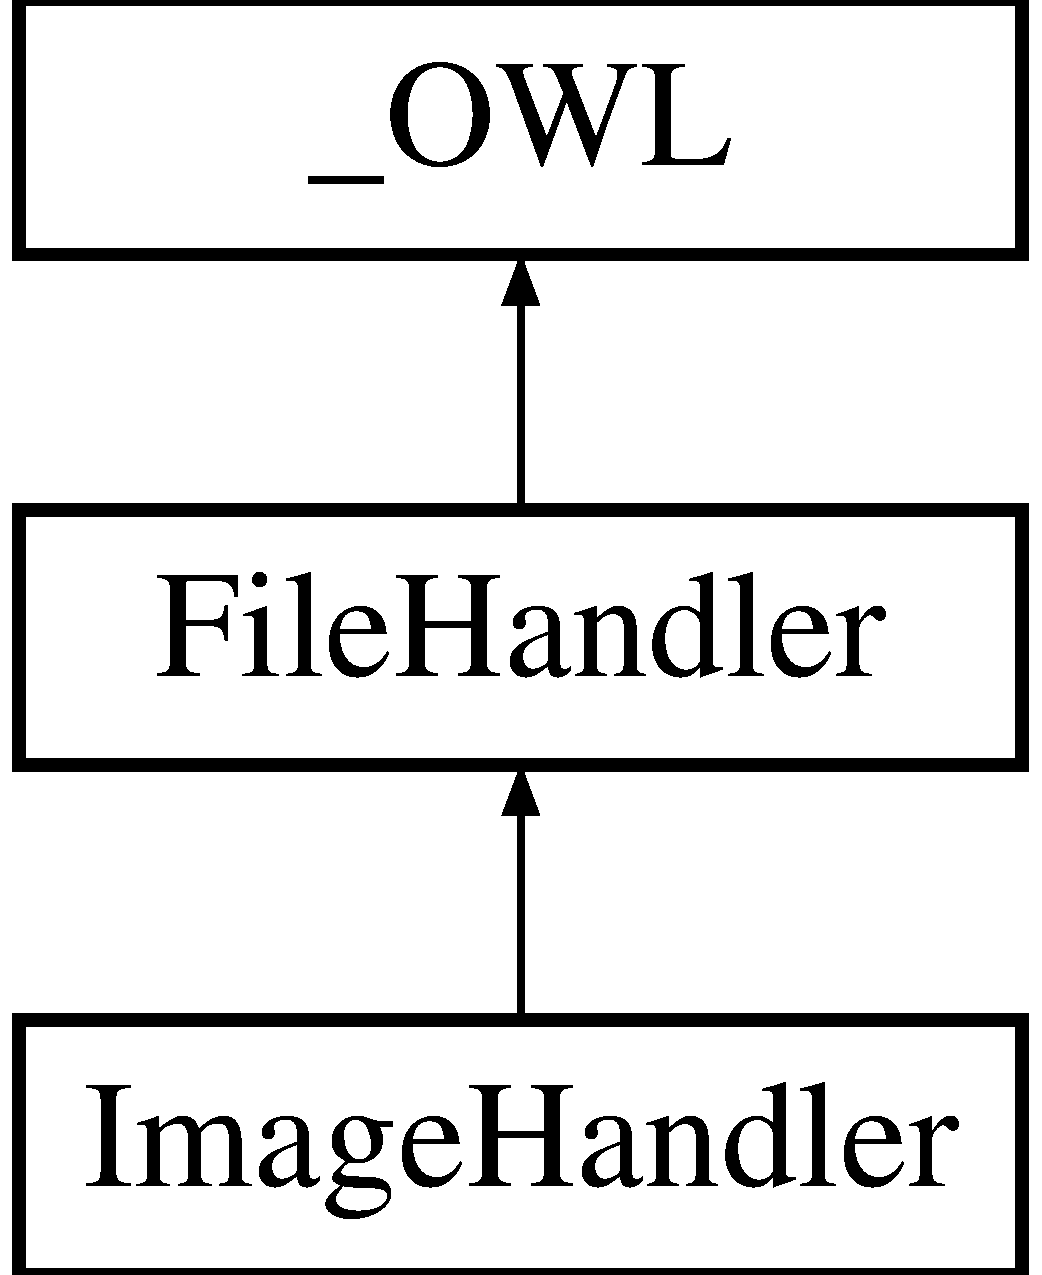
\includegraphics[height=3.000000cm]{classFileHandler}
\end{center}
\end{figure}
\subsection*{Public Member Functions}
\begin{DoxyCompactItemize}
\item 
{\bf \_\-\_\-construct} (\$name, \$req=false)
\item 
{\bf \_\-\_\-destruct} ()
\item 
{\bf encode} ()
\item 
{\bf download} ()
\item 
{\bf getLastWarning} ()
\item 
{\bf getStatus} ()
\item 
{\bf getSeverity} (\$status=null)
\item 
{\bf succeeded} (\$\_\-ok={\bf OWL\_\-SUCCESS}, \&\$\_\-object=null)
\item 
{\bf signal} (\$level={\bf OWL\_\-INFO}, \&\$text=false)
\item 
{\bf traceback} (\&\$text=false, \$depth=0)
\end{DoxyCompactItemize}
\subsection*{Public Attributes}
\begin{DoxyCompactItemize}
\item 
{\bf \$original\_\-name}
\end{DoxyCompactItemize}
\subsection*{Protected Member Functions}
\begin{DoxyCompactItemize}
\item 
{\bf open} (\$mode= 'r')
\item 
{\bf close} ()
\item 
{\bf readData} ()
\item 
{\bf readLine} (\$trim={\bf FILE\_\-NOTRIM})
\item 
{\bf init} ()
\item 
{\bf setCallback} (\$\_\-dispatcher)
\item 
{\bf setCallbackArgument} (array \$\_\-arg)
\item 
{\bf getCallback} ()
\item 
{\bf reset} ()
\item 
{\bf saveStatus} ()
\item 
{\bf restoreStatus} ()
\item 
{\bf check} (\&\$object, \$level={\bf OWL\_\-WARNING})
\item 
{\bf setStatus} (\$status, \$params=array())
\item 
{\bf setHighSeverity} (\&\$object=null)
\end{DoxyCompactItemize}
\subsection*{Protected Attributes}
\begin{DoxyCompactItemize}
\item 
{\bf \$name}
\item 
{\bf \$severity}
\end{DoxyCompactItemize}
\subsection*{Private Attributes}
\begin{DoxyCompactItemize}
\item 
{\bf \$fpointer}
\item 
{\bf \$opened}
\end{DoxyCompactItemize}


\subsection{Detailed Description}
File handler. 

Handle all files \begin{DoxyAuthor}{Author}
Oscar van Eijk, Oveas Functionality Provider 
\end{DoxyAuthor}
\begin{DoxyVersion}{Version}
May 15, 2007 -\/-\/ O van Eijk -\/-\/ initial version for Terra-\/Terra (based on an old OFM module) 

Jul 30, 2008 -\/-\/ O van Eijk -\/-\/ Modified version for OWL-\/PHP 
\end{DoxyVersion}


\subsection{Constructor \& Destructor Documentation}
\index{FileHandler@{FileHandler}!\_\-\_\-construct@{\_\-\_\-construct}}
\index{\_\-\_\-construct@{\_\-\_\-construct}!FileHandler@{FileHandler}}
\subsubsection[{\_\-\_\-construct}]{\setlength{\rightskip}{0pt plus 5cm}FileHandler::\_\-\_\-construct (
\begin{DoxyParamCaption}
\item[{\$}]{name, }
\item[{\$}]{req = {\ttfamily false}}
\end{DoxyParamCaption}
)}\label{classFileHandler_a8d75c8ea0c532acdeae0a0a4efa3704a}
Class constructor; setup the file characteristics 
\begin{DoxyParams}[1]{Parameters}
\mbox{\tt in}  & {\em \$name} & Filename \\
\hline
\mbox{\tt in}  & {\em \$req} & True is the file must exist at object create time \\
\hline
\end{DoxyParams}
\begin{DoxyAuthor}{Author}
Oscar van Eijk, Oveas Functionality Provider 
\end{DoxyAuthor}


Reimplemented in {\bf ImageHandler} \doxyref{}{p.}{classImageHandler_aa61dc81d4cf98eed31b32e2197018309}.



References \$name, \_\-OWL::init(), and \_\-OWL::setStatus().

\index{FileHandler@{FileHandler}!\_\-\_\-destruct@{\_\-\_\-destruct}}
\index{\_\-\_\-destruct@{\_\-\_\-destruct}!FileHandler@{FileHandler}}
\subsubsection[{\_\-\_\-destruct}]{\setlength{\rightskip}{0pt plus 5cm}FileHandler::\_\-\_\-destruct (
\begin{DoxyParamCaption}
{}
\end{DoxyParamCaption}
)}\label{classFileHandler_a734859e8962992da99dd8f853da5ae43}
Default class destructor \begin{DoxyAuthor}{Author}
Oscar van Eijk, Oveas Functionality Provider 
\end{DoxyAuthor}


Reimplemented from {\bf \_\-OWL} \doxyref{}{p.}{class__OWL_a44fd2222476a3109286cc82d92b6bbcc}.



References close().



\subsection{Member Function Documentation}
\index{FileHandler@{FileHandler}!check@{check}}
\index{check@{check}!FileHandler@{FileHandler}}
\subsubsection[{check}]{\setlength{\rightskip}{0pt plus 5cm}\_\-OWL::check (
\begin{DoxyParamCaption}
\item[{\&\$}]{object, }
\item[{\$}]{level = {\ttfamily {\bf OWL\_\-WARNING}}}
\end{DoxyParamCaption}
)\hspace{0.3cm}{\ttfamily  [protected, inherited]}}\label{class__OWL_ae2e3c56e5f3c4ce4156c6b1bb1c50f63}
This is a helper function for lazy developers. Some checks have to be made quite often, this is a kinda macro to handle that. It compares the own severity level with that of a given object. If the highest level is above a given max, a traceback and reset are performed.


\begin{DoxyParams}[1]{Parameters}
\mbox{\tt in}  & {\em \$object} & Pointer to an object to check against \\
\hline
\mbox{\tt in}  & {\em \$level} & The maximum severity level \\
\hline
\end{DoxyParams}
\begin{DoxyReturn}{Returns}
True if the severity level was correct (below the max), otherwise false 
\end{DoxyReturn}
\begin{DoxyAuthor}{Author}
Oscar van Eijk, Oveas Functionality Provider 
\end{DoxyAuthor}


References \_\-OWL::reset(), \_\-OWL::setHighSeverity(), and \_\-OWL::traceback().



Referenced by SessionHandler::write().

\index{FileHandler@{FileHandler}!close@{close}}
\index{close@{close}!FileHandler@{FileHandler}}
\subsubsection[{close}]{\setlength{\rightskip}{0pt plus 5cm}FileHandler::close (
\begin{DoxyParamCaption}
{}
\end{DoxyParamCaption}
)\hspace{0.3cm}{\ttfamily  [protected]}}\label{classFileHandler_aa48e7c3b67346e29b194d2f0ac5dd1f8}
Close the file \begin{DoxyAuthor}{Author}
Oscar van Eijk, Oveas Functionality Provider 
\end{DoxyAuthor}


References \_\-OWL::setStatus().



Referenced by \_\-\_\-destruct(), and readData().

\index{FileHandler@{FileHandler}!download@{download}}
\index{download@{download}!FileHandler@{FileHandler}}
\subsubsection[{download}]{\setlength{\rightskip}{0pt plus 5cm}FileHandler::download (
\begin{DoxyParamCaption}
{}
\end{DoxyParamCaption}
)}\label{classFileHandler_ac17edc9b92643c32ae6040b1235c64dd}
\index{FileHandler@{FileHandler}!encode@{encode}}
\index{encode@{encode}!FileHandler@{FileHandler}}
\subsubsection[{encode}]{\setlength{\rightskip}{0pt plus 5cm}FileHandler::encode (
\begin{DoxyParamCaption}
{}
\end{DoxyParamCaption}
)}\label{classFileHandler_aa29360bf94fd54d906256561f33d93ad}


References readData().

\index{FileHandler@{FileHandler}!getCallback@{getCallback}}
\index{getCallback@{getCallback}!FileHandler@{FileHandler}}
\subsubsection[{getCallback}]{\setlength{\rightskip}{0pt plus 5cm}\_\-OWL::getCallback (
\begin{DoxyParamCaption}
{}
\end{DoxyParamCaption}
)\hspace{0.3cm}{\ttfamily  [protected, inherited]}}\label{class__OWL_acb46ff88f43ca66f1268d3f5199c3f8d}
Retrieve a previously set (callback) dispatcher. The (callback) dispatcher is cleared immediatly. \begin{DoxyReturn}{Returns}
The dispatcher, of null on failure. 
\end{DoxyReturn}
\begin{DoxyAuthor}{Author}
Oscar van Eijk, Oveas Functionality Provider 
\end{DoxyAuthor}


Reimplemented in {\bf Dispatcher} \doxyref{}{p.}{classDispatcher_a31c4bd4e4eaee7ef90b1ea364a901447}.



References OWL::factory().

\index{FileHandler@{FileHandler}!getLastWarning@{getLastWarning}}
\index{getLastWarning@{getLastWarning}!FileHandler@{FileHandler}}
\subsubsection[{getLastWarning}]{\setlength{\rightskip}{0pt plus 5cm}\_\-OWL::getLastWarning (
\begin{DoxyParamCaption}
{}
\end{DoxyParamCaption}
)\hspace{0.3cm}{\ttfamily  [inherited]}}\label{class__OWL_a1888f52fc2d0ec29e146925ccad70a6b}
Get the last warning or error message. \begin{DoxyReturn}{Returns}
null if there was no error (severity below OWL\_\-WARNING), otherwise the error text. 
\end{DoxyReturn}
\begin{DoxyAuthor}{Author}
Oscar van Eijk, Oveas Functionality Provider 
\end{DoxyAuthor}


References \_\-OWL::signal().

\index{FileHandler@{FileHandler}!getSeverity@{getSeverity}}
\index{getSeverity@{getSeverity}!FileHandler@{FileHandler}}
\subsubsection[{getSeverity}]{\setlength{\rightskip}{0pt plus 5cm}\_\-OWL::getSeverity (
\begin{DoxyParamCaption}
\item[{\$}]{status = {\ttfamily null}}
\end{DoxyParamCaption}
)\hspace{0.3cm}{\ttfamily  [inherited]}}\label{class__OWL_a2374613f9bb7eccf49a5dbc9a9ef4751}
Get the current object severity level. 
\begin{DoxyParams}[1]{Parameters}
\mbox{\tt in}  & {\em \$status} & An optional parameter to check an other status code i.s.o the object's current status. \\
\hline
\end{DoxyParams}
\begin{DoxyReturn}{Returns}
Status severity level 
\end{DoxyReturn}
\begin{DoxyAuthor}{Author}
Oscar van Eijk, Oveas Functionality Provider 
\end{DoxyAuthor}


References \_\-OWL::\$status.



Referenced by LogHandler::composeMessage(), LogHandler::log(), and DataHandler::setKey().

\index{FileHandler@{FileHandler}!getStatus@{getStatus}}
\index{getStatus@{getStatus}!FileHandler@{FileHandler}}
\subsubsection[{getStatus}]{\setlength{\rightskip}{0pt plus 5cm}\_\-OWL::getStatus (
\begin{DoxyParamCaption}
{}
\end{DoxyParamCaption}
)\hspace{0.3cm}{\ttfamily  [final, inherited]}}\label{class__OWL_ac1f1643ff5b5db7c326c30477603358d}
Get the current object status. \begin{DoxyReturn}{Returns}
Object's status code 
\end{DoxyReturn}
\begin{DoxyAuthor}{Author}
Oscar van Eijk, Oveas Functionality Provider 
\end{DoxyAuthor}


Referenced by SchemeHandler::compare().

\index{FileHandler@{FileHandler}!init@{init}}
\index{init@{init}!FileHandler@{FileHandler}}
\subsubsection[{init}]{\setlength{\rightskip}{0pt plus 5cm}\_\-OWL::init (
\begin{DoxyParamCaption}
{}
\end{DoxyParamCaption}
)\hspace{0.3cm}{\ttfamily  [protected, inherited]}}\label{class__OWL_ae0ef3ded56e8a6b34b6461e5a721cd3e}
This function should be called by all constuctors. It initializes the general characteristics. Status is 'warning' by default, it's up to the contructor to set a proper status; if it's still 'warning', this $\ast$might$\ast$ indicate something went wrong. \begin{DoxyAuthor}{Author}
Oscar van Eijk, Oveas Functionality Provider 
\end{DoxyAuthor}


References OWL::factory(), and \_\-OWL::setStatus().



Referenced by FormFieldPlugin::\_\-\_\-construct(), Document::\_\-\_\-construct(), ContainerPlugin::\_\-\_\-construct(), Container::\_\-\_\-construct(), SocketHandler::\_\-\_\-construct(), SessionHandler::\_\-\_\-construct(), SchemeHandler::\_\-\_\-construct(), LogHandler::\_\-\_\-construct(), ImageHandler::\_\-\_\-construct(), FormHandler::\_\-\_\-construct(), \_\-\_\-construct(), DbHandler::\_\-\_\-construct(), HDataHandler::\_\-\_\-construct(), DataHandler::\_\-\_\-construct(), OWL::\_\-\_\-construct(), Mail::\_\-\_\-construct(), Group::\_\-\_\-construct(), Form::\_\-\_\-construct(), Dispatcher::\_\-\_\-construct(), and User::construct().

\index{FileHandler@{FileHandler}!open@{open}}
\index{open@{open}!FileHandler@{FileHandler}}
\subsubsection[{open}]{\setlength{\rightskip}{0pt plus 5cm}FileHandler::open (
\begin{DoxyParamCaption}
\item[{\$}]{mode = {\ttfamily 'r'}}
\end{DoxyParamCaption}
)\hspace{0.3cm}{\ttfamily  [protected]}}\label{classFileHandler_a2a650b033c4eb1f98ba47fb05ce7b454}
Open the file 
\begin{DoxyParams}[1]{Parameters}
\mbox{\tt in}  & {\em \$mode} & Mode in which the file should be opened:
\begin{DoxyItemize}
\item 'r' Open for reading only; place the file pointer at the beginning of the file.
\item 'r+' Open for reading and writing; place the file pointer at the beginning of the file.
\item 'w' Open for writing only; place the file pointer at the beginning of the file and truncate the file to zero length. If the file does not exist, attempt to create it.
\item 'w+' Open for reading and writing; place the file pointer at the beginning of the file and truncate the file to zero length. If the file does not exist, attempt to create it.
\item 'a' Open for writing only; place the file pointer at the end of the file. If the file does not exist, attempt to create it.
\item 'a+' Open for reading and writing; place the file pointer at the end of the file. If the file does not exist, attempt to create it. 
\end{DoxyItemize}\\
\hline
\end{DoxyParams}
\begin{DoxyAuthor}{Author}
Oscar van Eijk, Oveas Functionality Provider 
\end{DoxyAuthor}


References \_\-OWL::setStatus().



Referenced by readData().

\index{FileHandler@{FileHandler}!readData@{readData}}
\index{readData@{readData}!FileHandler@{FileHandler}}
\subsubsection[{readData}]{\setlength{\rightskip}{0pt plus 5cm}FileHandler::readData (
\begin{DoxyParamCaption}
{}
\end{DoxyParamCaption}
)\hspace{0.3cm}{\ttfamily  [protected]}}\label{classFileHandler_a6f9263704f08f071a5e563aeb3216d95}
Read the file contents and return as one dataset \begin{DoxyAuthor}{Author}
Oscar van Eijk, Oveas Functionality Provider 
\end{DoxyAuthor}


References close(), and open().



Referenced by encode().

\index{FileHandler@{FileHandler}!readLine@{readLine}}
\index{readLine@{readLine}!FileHandler@{FileHandler}}
\subsubsection[{readLine}]{\setlength{\rightskip}{0pt plus 5cm}FileHandler::readLine (
\begin{DoxyParamCaption}
\item[{\$}]{trim = {\ttfamily {\bf FILE\_\-NOTRIM}}}
\end{DoxyParamCaption}
)\hspace{0.3cm}{\ttfamily  [protected]}}\label{classFileHandler_a2140ee43c68f088396b4573a56e3007c}
Read a single line from the file. File must be opened before 
\begin{DoxyParams}[1]{Parameters}
\mbox{\tt in}  & {\em \$trim} & specify how the returned line should be trimmed:
\begin{DoxyItemize}
\item FILE\_\-NOTRIM
\item FILE\_\-TRIM\_\-L
\item FILE\_\-TRIM\_\-R
\item FILE\_\-TRIM\_\-C 
\end{DoxyItemize}\\
\hline
\end{DoxyParams}
\begin{DoxyAuthor}{Author}
Oscar van Eijk, Oveas Functionality Provider 
\end{DoxyAuthor}


References \_\-OWL::setStatus().

\index{FileHandler@{FileHandler}!reset@{reset}}
\index{reset@{reset}!FileHandler@{FileHandler}}
\subsubsection[{reset}]{\setlength{\rightskip}{0pt plus 5cm}\_\-OWL::reset (
\begin{DoxyParamCaption}
{}
\end{DoxyParamCaption}
)\hspace{0.3cm}{\ttfamily  [protected, inherited]}}\label{class__OWL_a2f2a042bcf31965194c03033df0edc9b}
General reset function for all objects. Should be called after each non-\/fatal error \begin{DoxyAuthor}{Author}
Oscar van Eijk, Oveas Functionality Provider 
\end{DoxyAuthor}


Reimplemented in {\bf DbHandler} \doxyref{}{p.}{classDbHandler_a9982df4830f05803935bb31bac7fae3d}, and {\bf SchemeHandler} \doxyref{}{p.}{classSchemeHandler_aa25feb4a70d67b3d571904be4b2f50bc}.



References \_\-OWL::resetCalltree().



Referenced by \_\-OWL::check(), SessionHandler::read(), DataHandler::reset(), and \_\-OWL::setStatus().

\index{FileHandler@{FileHandler}!restoreStatus@{restoreStatus}}
\index{restoreStatus@{restoreStatus}!FileHandler@{FileHandler}}
\subsubsection[{restoreStatus}]{\setlength{\rightskip}{0pt plus 5cm}\_\-OWL::restoreStatus (
\begin{DoxyParamCaption}
{}
\end{DoxyParamCaption}
)\hspace{0.3cm}{\ttfamily  [protected, inherited]}}\label{class__OWL_a93de01a9bbbc3f228e1a62a0740e90f0}
Restore the previously saved status object and destroy the copy \begin{DoxyAuthor}{Author}
Oscar van Eijk, Oveas Functionality Provider 
\end{DoxyAuthor}


References \_\-OWL::setStatus().



Referenced by User::logout().

\index{FileHandler@{FileHandler}!saveStatus@{saveStatus}}
\index{saveStatus@{saveStatus}!FileHandler@{FileHandler}}
\subsubsection[{saveStatus}]{\setlength{\rightskip}{0pt plus 5cm}\_\-OWL::saveStatus (
\begin{DoxyParamCaption}
{}
\end{DoxyParamCaption}
)\hspace{0.3cm}{\ttfamily  [protected, inherited]}}\label{class__OWL_add923dc756471318edca8883db3f4420}
Create a copy of the status object \begin{DoxyAuthor}{Author}
Oscar van Eijk, Oveas Functionality Provider 
\end{DoxyAuthor}


Referenced by User::logout().

\index{FileHandler@{FileHandler}!setCallback@{setCallback}}
\index{setCallback@{setCallback}!FileHandler@{FileHandler}}
\subsubsection[{setCallback}]{\setlength{\rightskip}{0pt plus 5cm}\_\-OWL::setCallback (
\begin{DoxyParamCaption}
\item[{\$}]{\_\-dispatcher}
\end{DoxyParamCaption}
)\hspace{0.3cm}{\ttfamily  [protected, inherited]}}\label{class__OWL_a5f84d43cd4dc7810649f1e2ebecad360}
Set a dispatcher for later callback 
\begin{DoxyParams}[1]{Parameters}
\mbox{\tt in}  & {\em \$\_\-dispatcher} & Dispatched, \\
\hline
\end{DoxyParams}
\begin{DoxySeeAlso}{See also}
\doxyref{Dispatcher::composeDispatcher()}{p.}{classDispatcher_a8a974bbbb30be7cda74f9929972fd2f6} 
\end{DoxySeeAlso}
\begin{DoxyReturn}{Returns}
True on success, false on failure 
\end{DoxyReturn}
\begin{DoxyAuthor}{Author}
Oscar van Eijk, Oveas Functionality Provider 
\end{DoxyAuthor}


References OWL::factory().

\index{FileHandler@{FileHandler}!setCallbackArgument@{setCallbackArgument}}
\index{setCallbackArgument@{setCallbackArgument}!FileHandler@{FileHandler}}
\subsubsection[{setCallbackArgument}]{\setlength{\rightskip}{0pt plus 5cm}\_\-OWL::setCallbackArgument (
\begin{DoxyParamCaption}
\item[{array \$}]{\_\-arg}
\end{DoxyParamCaption}
)\hspace{0.3cm}{\ttfamily  [protected, inherited]}}\label{class__OWL_a4e9ebfbd3c0d76539bed4e44de9962c3}
Add an argument to a previously registered callback dispatcher 
\begin{DoxyParams}[1]{Parameters}
\mbox{\tt in}  & {\em \$\_\-arg} & Argument, must be an array type. When non-\/ arrays should be passed as arguments, the must be set when the callback is registered already \\
\hline
\end{DoxyParams}
\begin{DoxyReturn}{Returns}
True on success, false on failure 
\end{DoxyReturn}
\begin{DoxyAuthor}{Author}
Oscar van Eijk, Oveas Functionality Provider 
\end{DoxyAuthor}


References OWL::factory().



Referenced by User::register().

\index{FileHandler@{FileHandler}!setHighSeverity@{setHighSeverity}}
\index{setHighSeverity@{setHighSeverity}!FileHandler@{FileHandler}}
\subsubsection[{setHighSeverity}]{\setlength{\rightskip}{0pt plus 5cm}\_\-OWL::setHighSeverity (
\begin{DoxyParamCaption}
\item[{\&\$}]{object = {\ttfamily null}}
\end{DoxyParamCaption}
)\hspace{0.3cm}{\ttfamily  [protected, inherited]}}\label{class__OWL_a97173dbe452428d3851406413264734d}
Compare the severity level of the current object with a given one and set my statuspointer to the object with the highest level. \begin{DoxyAuthor}{Author}
Oscar van Eijk, Oveas Functionality Provider 
\end{DoxyAuthor}


Referenced by \_\-OWL::check(), DataHandler::db(), DataHandler::prepare(), and SessionHandler::read().

\index{FileHandler@{FileHandler}!setStatus@{setStatus}}
\index{setStatus@{setStatus}!FileHandler@{FileHandler}}
\subsubsection[{setStatus}]{\setlength{\rightskip}{0pt plus 5cm}\_\-OWL::setStatus (
\begin{DoxyParamCaption}
\item[{\$}]{status, }
\item[{\$}]{params = {\ttfamily array~()}}
\end{DoxyParamCaption}
)\hspace{0.3cm}{\ttfamily  [final, protected, inherited]}}\label{class__OWL_a80e2fe01c3663dbb0ab685eebe33fd1e}
Set the current object status to the specified value. 
\begin{DoxyParams}[1]{Parameters}
\mbox{\tt in}  & {\em \$status} & \doxyref{OWL}{p.}{classOWL} status code \\
\hline
\mbox{\tt in}  & {\em \$params} & \\
\hline
\end{DoxyParams}
\begin{DoxyAuthor}{Author}
Oscar van Eijk, Oveas Functionality Provider 
\end{DoxyAuthor}


References \$GLOBALS, \_\-OWL::\$status, ConfigHandler::get(), Register::getCode(), \_\-OWL::reset(), and \_\-OWL::signal().



Referenced by DbHandler::\_\-\_\-clone(), Container::\_\-\_\-construct(), SocketHandler::\_\-\_\-construct(), SchemeHandler::\_\-\_\-construct(), ImageHandler::\_\-\_\-construct(), FormHandler::\_\-\_\-construct(), \_\-\_\-construct(), DbHandler::\_\-\_\-construct(), DataHandler::\_\-\_\-construct(), Session::\_\-\_\-construct(), Mail::\_\-\_\-construct(), BaseElement::\_\-getContent(), HDataHandler::\_\-getNewLeft(), Mail::addBcc(), Mail::addCc(), Container::addContainer(), Form::addField(), FormFieldRadioPlugin::addOption(), HDataHandler::addParent(), Mail::addTo(), BaseElement::addToContent(), DbHandler::alt(), SchemeHandler::alterScheme(), close(), DbHandler::commitTransaction(), Dispatcher::composeDispatcher(), User::confirm(), SocketHandler::connect(), DbHandler::connect(), DbHandler::create(), SchemeHandler::createScheme(), DbHandler::dbread(), SchemeHandler::defineIndex(), SchemeHandler::defineScheme(), SocketHandler::disconnect(), Dispatcher::dispatch(), HDataHandler::enableCrossLink(), FormHandler::get(), DataHandler::get(), HDataHandler::getDirectChildren(), HDataHandler::getFullOffspring(), Group::getGroupByName(), SchemeHandler::getTableColumns(), SchemeHandler::getTableIndexes(), \_\-OWL::init(), Document::loadScript(), Document::loadStyle(), DbHandler::lockTable(), User::login(), HDataHandler::moveNode(), open(), DbHandler::open(), LogHandler::openLogfile(), DataHandler::prepare(), DbHandler::prepareDelete(), DbHandler::prepareField(), DbHandler::prepareInsert(), DbHandler::prepareRead(), DbHandler::prepareUpdate(), SocketHandler::read(), DbHandler::read(), readLine(), HDataHandler::readQuery(), User::readUserdata(), User::register(), Dispatcher::registerArgument(), Dispatcher::registerCallback(), DbHandler::resetTable(), \_\-OWL::restoreStatus(), DbHandler::rollbackTransaction(), SchemeHandler::scheme(), Mail::send(), FormHandler::set(), BaseElement::setAttributes(), BaseElement::setContent(), Form::setEncoding(), Document::setFavicon(), Form::setFieldAttributes(), Mail::setFrom(), DataHandler::setJoin(), DataHandler::setKey(), FormFieldTextPlugin::setMaxsize(), Document::setMeta(), Form::setMethod(), FormFieldRadioPlugin::setSelected(), Mail::setSender(), FormFieldTextPlugin::setSize(), FormFieldSelectPlugin::setSize(), FormFieldSelectPlugin::setValue(), Form::showField(), DbHandler::startTransaction(), SchemeHandler::tableDescription(), DbHandler::unlockTable(), SchemeHandler::validateScheme(), SocketHandler::write(), DbHandler::write(), and HDataHandler::writeQuery().

\index{FileHandler@{FileHandler}!signal@{signal}}
\index{signal@{signal}!FileHandler@{FileHandler}}
\subsubsection[{signal}]{\setlength{\rightskip}{0pt plus 5cm}\_\-OWL::signal (
\begin{DoxyParamCaption}
\item[{\$}]{level = {\ttfamily {\bf OWL\_\-INFO}}, }
\item[{\&\$}]{text = {\ttfamily false}}
\end{DoxyParamCaption}
)\hspace{0.3cm}{\ttfamily  [inherited]}}\label{class__OWL_a51ba4a16409acf2a2f61f286939091a5}
Display the message for the current object status 
\begin{DoxyParams}[1]{Parameters}
\mbox{\tt in}  & {\em \$level} & An optional severity level; message will only be displayed when it is at least of this level. \\
\hline
\mbox{\tt out}  & {\em \$text} & If this parameter is given, the message text is returned in this string instead of echood. \\
\hline
\end{DoxyParams}
\begin{DoxyReturn}{Returns}
The severity level for this object 
\end{DoxyReturn}
\begin{DoxyAuthor}{Author}
Oscar van Eijk, Oveas Functionality Provider 
\end{DoxyAuthor}


References ConfigHandler::get().



Referenced by \_\-OWL::getLastWarning(), \_\-OWL::setStatus(), and \_\-OWL::traceback().

\index{FileHandler@{FileHandler}!succeeded@{succeeded}}
\index{succeeded@{succeeded}!FileHandler@{FileHandler}}
\subsubsection[{succeeded}]{\setlength{\rightskip}{0pt plus 5cm}\_\-OWL::succeeded (
\begin{DoxyParamCaption}
\item[{\$}]{\_\-ok = {\ttfamily {\bf OWL\_\-SUCCESS}}, }
\item[{\&\$}]{\_\-object = {\ttfamily null}}
\end{DoxyParamCaption}
)\hspace{0.3cm}{\ttfamily  [inherited]}}\label{class__OWL_a53ab4d3bbb2c6a56966c339ca4b4c805}
Check if the object currenlty has a success state 
\begin{DoxyParams}[1]{Parameters}
\mbox{\tt in}  & {\em \$\_\-ok} & The highest severity that's considered successfull, default OWL\_\-SUCCESS \\
\hline
\mbox{\tt in}  & {\em \$\_\-object} & REference to the object to check, defaults to the current object \\
\hline
\end{DoxyParams}
\begin{DoxyReturn}{Returns}
Boolean true when successfull 
\end{DoxyReturn}
\begin{DoxyAuthor}{Author}
Oscar van Eijk, Oveas Functionality Provider 
\end{DoxyAuthor}


Referenced by User::construct(), Dispatcher::registerArgument(), and Dispatcher::registerCallback().

\index{FileHandler@{FileHandler}!traceback@{traceback}}
\index{traceback@{traceback}!FileHandler@{FileHandler}}
\subsubsection[{traceback}]{\setlength{\rightskip}{0pt plus 5cm}\_\-OWL::traceback (
\begin{DoxyParamCaption}
\item[{\&\$}]{text = {\ttfamily false}, }
\item[{\$}]{depth = {\ttfamily 0}}
\end{DoxyParamCaption}
)\hspace{0.3cm}{\ttfamily  [inherited]}}\label{class__OWL_aa29547995d6741b7d2b90c1d4ea99a13}
If somehwere in the nested calls an error occured, we can traceback the original failing object with this function and signal the message. 
\begin{DoxyParams}[1]{Parameters}
\mbox{\tt out}  & {\em \$text} & Optional variable in which the message text can be stored. If not given, the text will be written to standard output \\
\hline
\mbox{\tt in}  & {\em \$depth} & This paramater should be initially empty. It calculates the depth in recursive calls. \\
\hline
\end{DoxyParams}
\begin{DoxyReturn}{Returns}
Severity code of the failing object 
\end{DoxyReturn}
\begin{DoxyAuthor}{Author}
Oscar van Eijk, Oveas Functionality Provider 
\end{DoxyAuthor}


References \_\-OWL::signal().



Referenced by \_\-OWL::check(), User::login(), and SessionHandler::read().



\subsection{Member Data Documentation}
\index{FileHandler@{FileHandler}!\$fpointer@{\$fpointer}}
\index{\$fpointer@{\$fpointer}!FileHandler@{FileHandler}}
\subsubsection[{\$fpointer}]{\setlength{\rightskip}{0pt plus 5cm}FileHandler::\$fpointer\hspace{0.3cm}{\ttfamily  [private]}}\label{classFileHandler_aa0aa66fd3ad551b3f508b901a95c0c2d}
Pointer to te file when opened 

Reimplemented in {\bf ImageHandler} \doxyref{}{p.}{classImageHandler_ac56acda82f7ece75d33f6c57845a727e}.

\index{FileHandler@{FileHandler}!\$name@{\$name}}
\index{\$name@{\$name}!FileHandler@{FileHandler}}
\subsubsection[{\$name}]{\setlength{\rightskip}{0pt plus 5cm}FileHandler::\$name\hspace{0.3cm}{\ttfamily  [protected]}}\label{classFileHandler_a94903bd51b241928ed415ad271c38805}
Full filename as stored on the file system 

Reimplemented in {\bf ImageHandler} \doxyref{}{p.}{classImageHandler_a517b3d7ff8643cca1dc2080523bfe2d6}.



Referenced by \_\-\_\-construct().

\index{FileHandler@{FileHandler}!\$opened@{\$opened}}
\index{\$opened@{\$opened}!FileHandler@{FileHandler}}
\subsubsection[{\$opened}]{\setlength{\rightskip}{0pt plus 5cm}FileHandler::\$opened\hspace{0.3cm}{\ttfamily  [private]}}\label{classFileHandler_a061409b2bbd2e13bc47415527c0de720}
Boolean that's true when the file is opened 

Reimplemented in {\bf ImageHandler} \doxyref{}{p.}{classImageHandler_a6a87b3626bd0a457c6937b3e9b1cc69b}.

\index{FileHandler@{FileHandler}!\$original\_\-name@{\$original\_\-name}}
\index{\$original\_\-name@{\$original\_\-name}!FileHandler@{FileHandler}}
\subsubsection[{\$original\_\-name}]{\setlength{\rightskip}{0pt plus 5cm}FileHandler::\$original\_\-name}\label{classFileHandler_a477708585850c3c8725ccf56bfe0b4a8}


Reimplemented in {\bf ImageHandler} \doxyref{}{p.}{classImageHandler_a1712c9444d65879aab111260767afaab}.

\index{FileHandler@{FileHandler}!\$severity@{\$severity}}
\index{\$severity@{\$severity}!FileHandler@{FileHandler}}
\subsubsection[{\$severity}]{\setlength{\rightskip}{0pt plus 5cm}\_\-OWL::\$severity\hspace{0.3cm}{\ttfamily  [protected, inherited]}}\label{class__OWL_ad26b40a9dbbacb33e299b17826f8327c}
Severity level of the current object status 

The documentation for this class was generated from the following file:\begin{DoxyCompactItemize}
\item 
/home/oscar/projects/owl-\/php/src/kernel/so/{\bf class.filehandler.php}\end{DoxyCompactItemize}

\section{SessionHandler Class Reference}
\label{classSessionHandler}\index{SessionHandler@{SessionHandler}}


the PHP session object  




Inheritance diagram for SessionHandler:\nopagebreak
\begin{figure}[H]
\begin{center}
\leavevmode
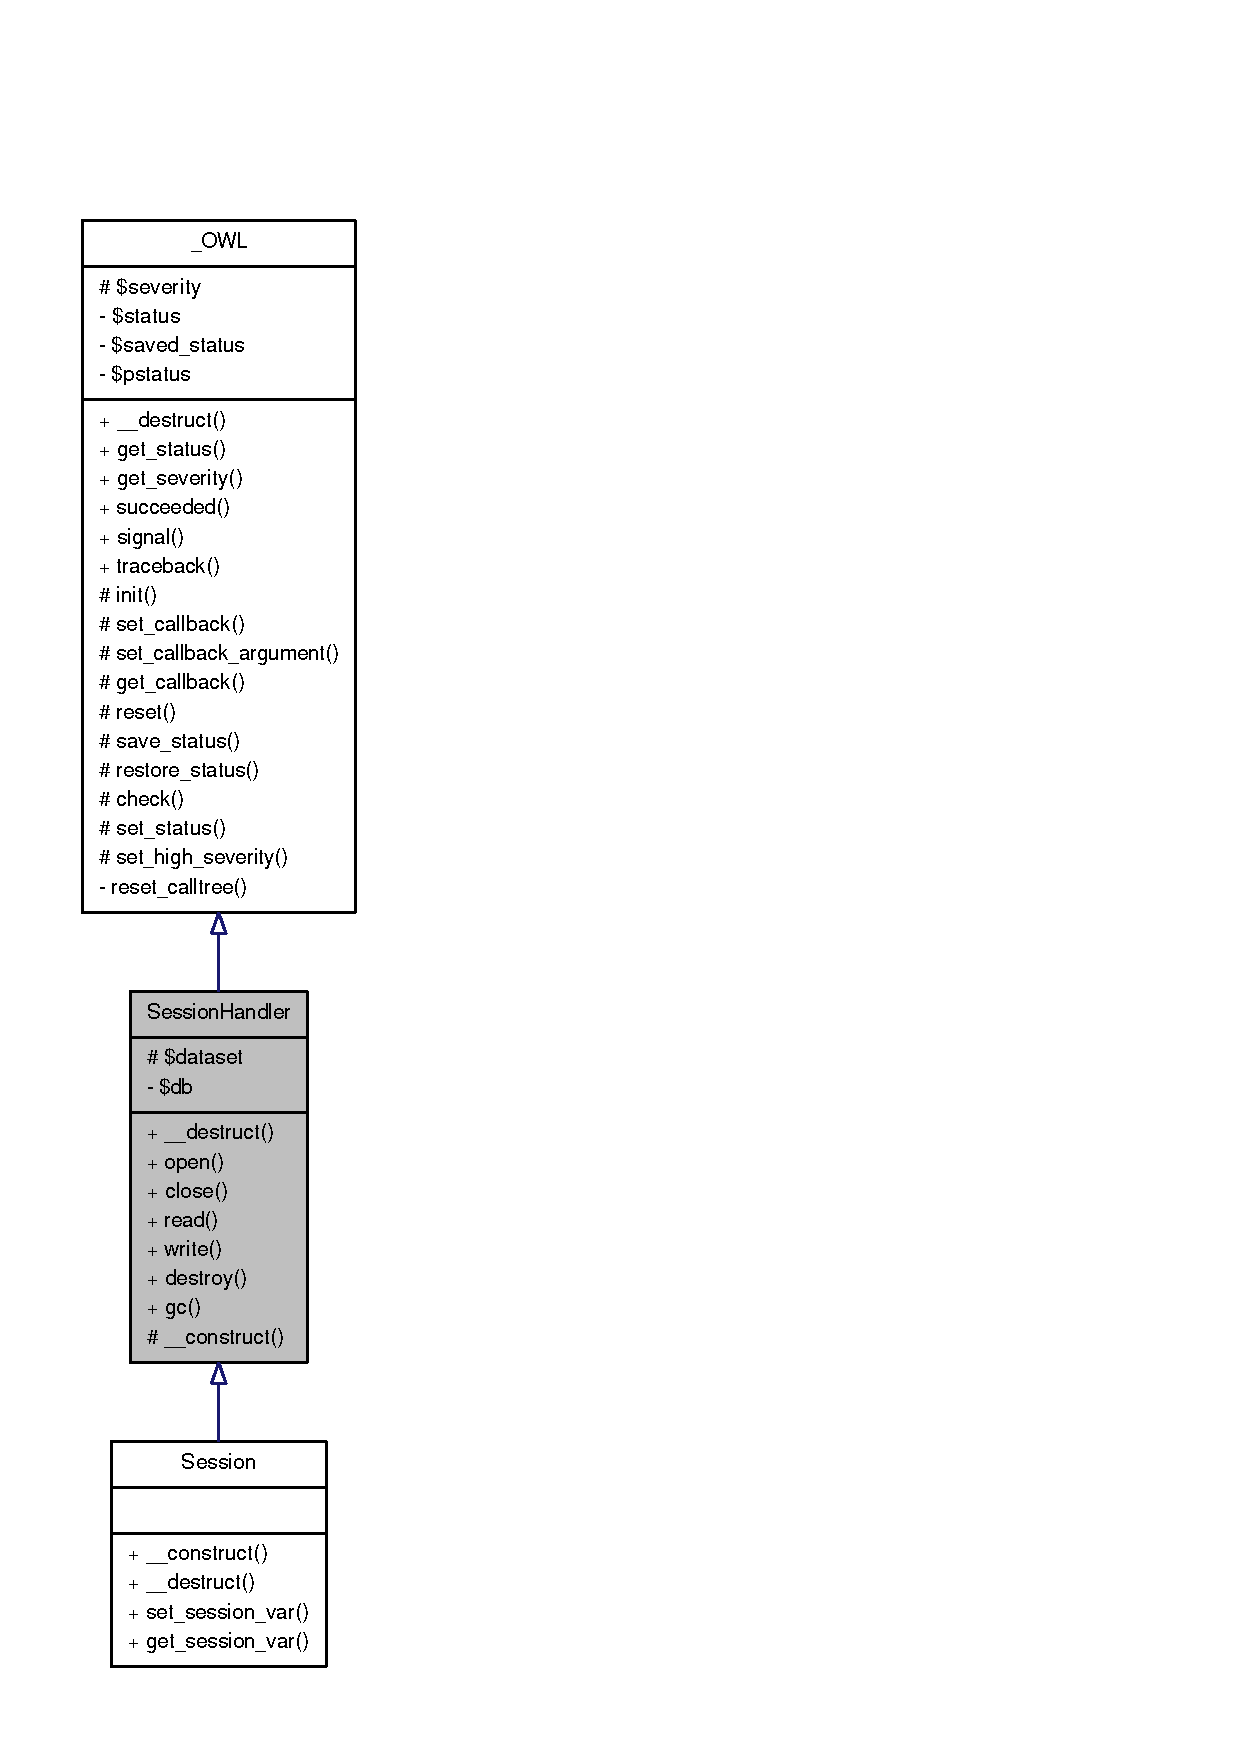
\includegraphics[height=400pt]{classSessionHandler__inherit__graph}
\end{center}
\end{figure}


Collaboration diagram for SessionHandler:\nopagebreak
\begin{figure}[H]
\begin{center}
\leavevmode
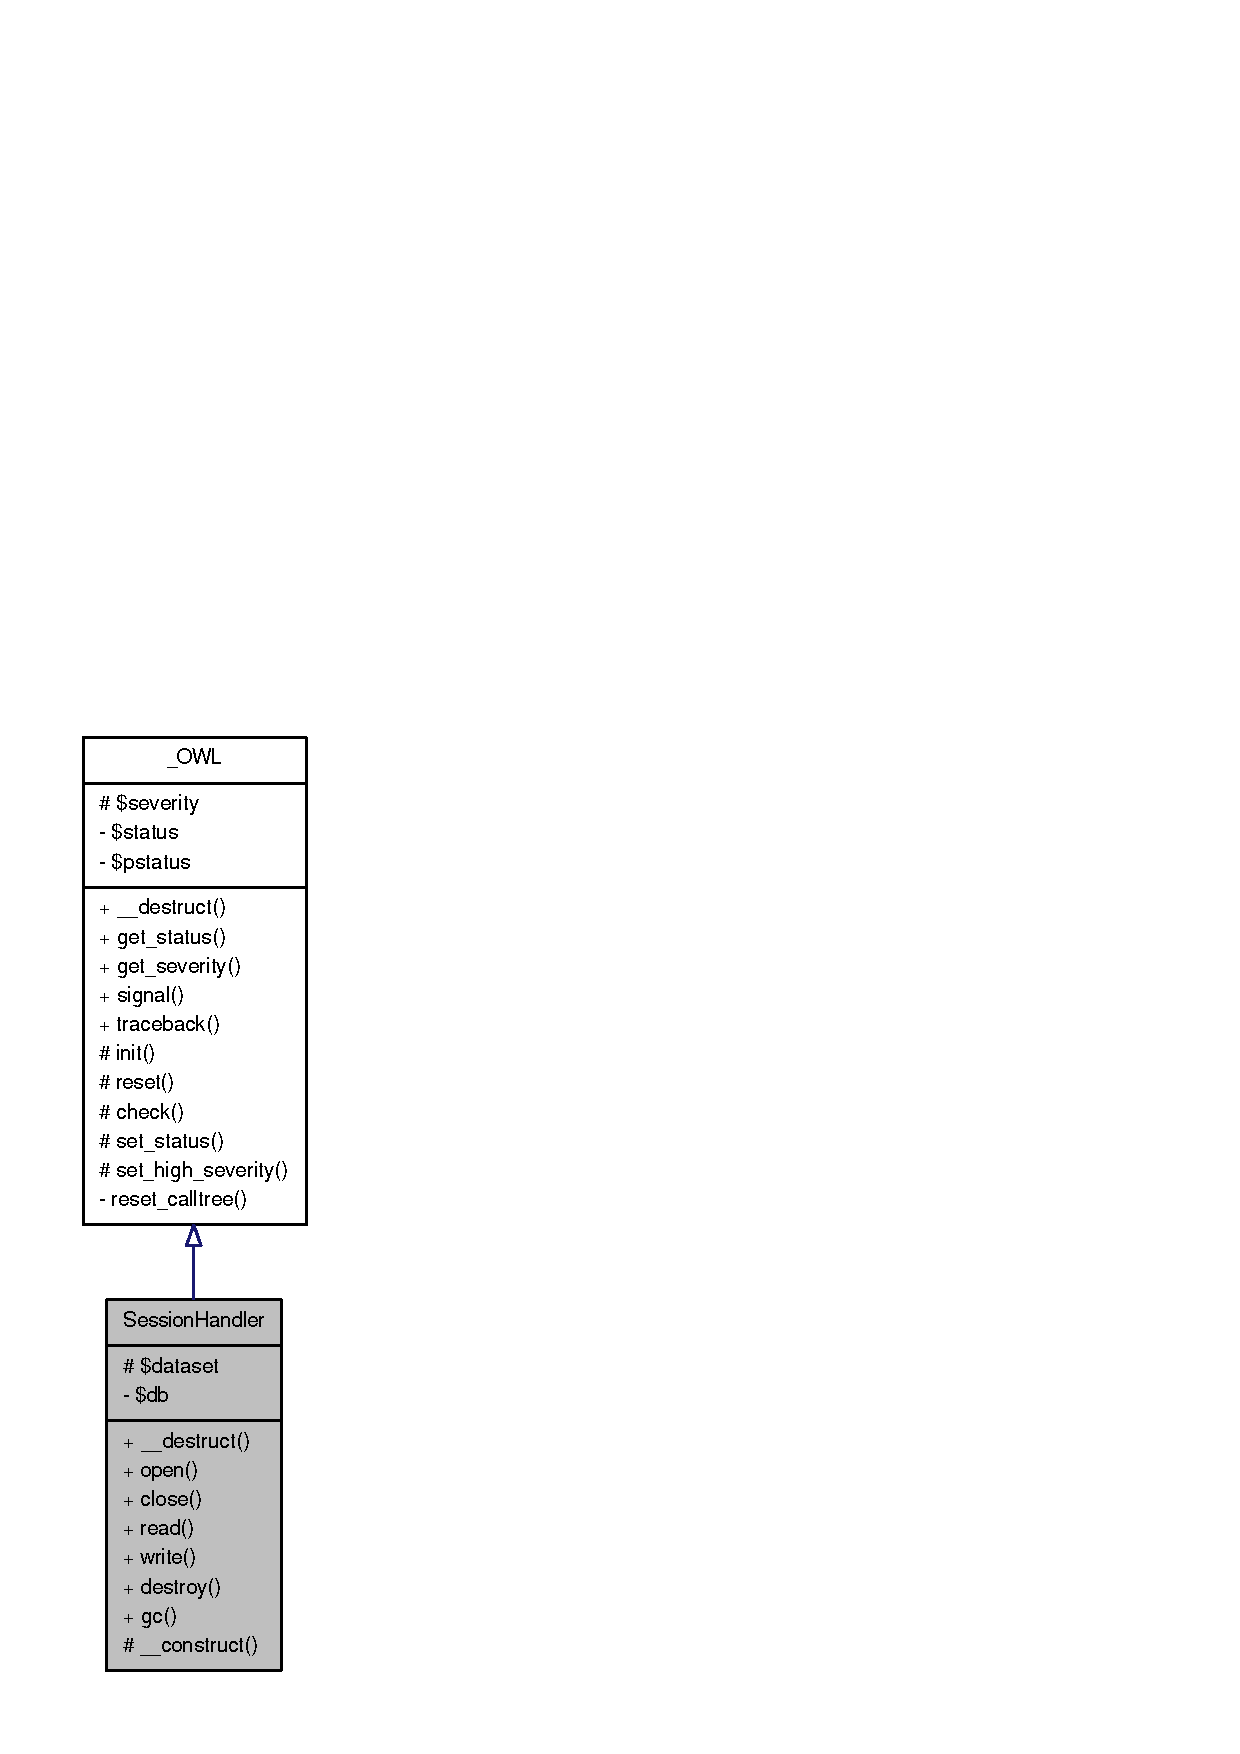
\includegraphics[height=400pt]{classSessionHandler__coll__graph}
\end{center}
\end{figure}
\subsection*{Public Member Functions}
\begin{DoxyCompactItemize}
\item 
\hyperlink{classSessionHandler_a461097c3ee6b1aecf833ce1225d02329}{\_\-\_\-destruct} ()
\item 
\hyperlink{classSessionHandler_a50aa0b123f53d99de350a0eb02b4bfa5}{open} ()
\item 
\hyperlink{classSessionHandler_a335ced83731c7e3e685b7e0df2989c79}{close} ()
\item 
\hyperlink{classSessionHandler_a58cc3e5bf5b14e7bfbc73162de1f5d2b}{read} (\$id)
\item 
\hyperlink{classSessionHandler_ab59071ef0d3deee2472c6916471bd9f5}{write} (\$id, \$data)
\item 
\hyperlink{classSessionHandler_a4e43712ef307979de1b12039ef801adb}{destroy} (\$id)
\item 
\hyperlink{classSessionHandler_ac33097332375ae3f8a43c31cef6db0e8}{gc} (\$lifetime)
\item 
\hyperlink{class__OWL_a99ec771fa2c5c279f80152cc09e489a8}{get\_\-status} ()
\item 
\hyperlink{class__OWL_adf9509ef96858be7bdd9414c5ef129aa}{get\_\-severity} (\$status=null)
\item 
\hyperlink{class__OWL_a51ba4a16409acf2a2f61f286939091a5}{signal} (\$level=\hyperlink{owl_8severitycodes_8php_a139328861128689f2f4def6a399d9057}{OWL\_\-INFO}, \&\$text=false)
\item 
\hyperlink{class__OWL_aa29547995d6741b7d2b90c1d4ea99a13}{traceback} (\&\$text=false, \$depth=0)
\end{DoxyCompactItemize}
\subsection*{Protected Member Functions}
\begin{DoxyCompactItemize}
\item 
\hyperlink{classSessionHandler_a546ba6d31a1ce532de13f65aadc3be0e}{\_\-\_\-construct} ()
\item 
\hyperlink{class__OWL_ae0ef3ded56e8a6b34b6461e5a721cd3e}{init} ()
\item 
\hyperlink{class__OWL_a2f2a042bcf31965194c03033df0edc9b}{reset} ()
\item 
\hyperlink{class__OWL_ad6f4f6946f40199dd0333cf219fa500e}{check} (\&\$object, \$level)
\item 
\hyperlink{class__OWL_aea912d0ede9b3c2a69b79072d94d4787}{set\_\-status} (\$status, \$params=array())
\item 
\hyperlink{class__OWL_a576829692a3b66e3d518853bf43abae3}{set\_\-high\_\-severity} (\&\$object=null)
\end{DoxyCompactItemize}
\subsection*{Protected Attributes}
\begin{DoxyCompactItemize}
\item 
\hyperlink{classSessionHandler_a74c46fcfbadd4c4e6bacc73ddf350056}{\$dataset}
\item 
\hyperlink{class__OWL_ad26b40a9dbbacb33e299b17826f8327c}{\$severity}
\end{DoxyCompactItemize}
\subsection*{Private Attributes}
\begin{DoxyCompactItemize}
\item 
\hyperlink{classSessionHandler_a0bb7c3206f3664f2a4b8e96edf49a3bc}{\$db}
\end{DoxyCompactItemize}


\subsection{Detailed Description}
the PHP session object This class saves and (re)stores the user sessions \begin{DoxyAuthor}{Author}
Oscar van Eijk, Oveas Functionality Provider 
\end{DoxyAuthor}
\begin{DoxyVersion}{Version}
Jul 29, 2008 -\/-\/ O van Eijk -\/-\/ initial version 
\end{DoxyVersion}


\subsection{Constructor \& Destructor Documentation}
\index{SessionHandler@{SessionHandler}!\_\-\_\-construct@{\_\-\_\-construct}}
\index{\_\-\_\-construct@{\_\-\_\-construct}!SessionHandler@{SessionHandler}}
\subsubsection[{\_\-\_\-construct}]{\setlength{\rightskip}{0pt plus 5cm}SessionHandler::\_\-\_\-construct ()\hspace{0.3cm}{\ttfamily  \mbox{[}protected\mbox{]}}}\label{classSessionHandler_a546ba6d31a1ce532de13f65aadc3be0e}
Class constructor; set the save\_\-handler 

Reimplemented in \hyperlink{classSession_a36373ba15d6c8f932aeea02d7320d7c8}{Session}.



References DbHandler::get\_\-instance(), \_\-OWL::init(), and \_\-OWL::set\_\-status().

\index{SessionHandler@{SessionHandler}!\_\-\_\-destruct@{\_\-\_\-destruct}}
\index{\_\-\_\-destruct@{\_\-\_\-destruct}!SessionHandler@{SessionHandler}}
\subsubsection[{\_\-\_\-destruct}]{\setlength{\rightskip}{0pt plus 5cm}SessionHandler::\_\-\_\-destruct ()}\label{classSessionHandler_a461097c3ee6b1aecf833ce1225d02329}
Write the session data back to the database 

Reimplemented from \hyperlink{class__OWL_a44fd2222476a3109286cc82d92b6bbcc}{\_\-OWL}.



Reimplemented in \hyperlink{classSession_aa498272c85524e4700abc3363883165b}{Session}.



\subsection{Member Function Documentation}
\index{SessionHandler@{SessionHandler}!check@{check}}
\index{check@{check}!SessionHandler@{SessionHandler}}
\subsubsection[{check}]{\setlength{\rightskip}{0pt plus 5cm}\_\-OWL::check (\&\$ {\em object}, \/  \$ {\em level})\hspace{0.3cm}{\ttfamily  \mbox{[}protected, inherited\mbox{]}}}\label{class__OWL_ad6f4f6946f40199dd0333cf219fa500e}
This is a helper function for lazy developers. Some checks have to be made quite often, this is a kinda macro to handle that. It compares the own severity level with that of a given object. If the highest level is above a given max, a traceback and reset are performed.


\begin{DoxyParams}{Parameters}
\item[\mbox{$\leftarrow$} {\em \$object}]Pointer to an object to check against \item[\mbox{$\leftarrow$} {\em \$level}]The maximum severity level \end{DoxyParams}
\begin{DoxyReturn}{Returns}
True if the severity level was correct ( below the max), otherwise false 
\end{DoxyReturn}


References \_\-OWL::reset(), \_\-OWL::set\_\-high\_\-severity(), and \_\-OWL::traceback().



Referenced by write().

\index{SessionHandler@{SessionHandler}!close@{close}}
\index{close@{close}!SessionHandler@{SessionHandler}}
\subsubsection[{close}]{\setlength{\rightskip}{0pt plus 5cm}SessionHandler::close ()}\label{classSessionHandler_a335ced83731c7e3e685b7e0df2989c79}
Close the session

\begin{DoxyReturn}{Returns}
bool 
\end{DoxyReturn}
\index{SessionHandler@{SessionHandler}!destroy@{destroy}}
\index{destroy@{destroy}!SessionHandler@{SessionHandler}}
\subsubsection[{destroy}]{\setlength{\rightskip}{0pt plus 5cm}SessionHandler::destroy (\$ {\em id})}\label{classSessionHandler_a4e43712ef307979de1b12039ef801adb}
Destroy a session


\begin{DoxyParams}{Parameters}
\item[\mbox{$\leftarrow$} {\em \$id}]ID of the session to destroy \end{DoxyParams}
\begin{DoxyReturn}{Returns}
Boolean indicating success (true) or failure (false) 
\end{DoxyReturn}
\index{SessionHandler@{SessionHandler}!gc@{gc}}
\index{gc@{gc}!SessionHandler@{SessionHandler}}
\subsubsection[{gc}]{\setlength{\rightskip}{0pt plus 5cm}SessionHandler::gc (\$ {\em lifetime})}\label{classSessionHandler_ac33097332375ae3f8a43c31cef6db0e8}
Garbage Collector. By default, this has a 1\% change of being executed (session.gc\_\-probability/session.gc\_\-divisor). The values can be changed in the constructor.


\begin{DoxyParams}{Parameters}
\item[\mbox{$\leftarrow$} {\em \$lifetime}]\hyperlink{classSession}{Session} lifetime in seconds. By default, 1440 seconds. This can be changed in the constructor \end{DoxyParams}
\begin{DoxyReturn}{Returns}
Status code 
\end{DoxyReturn}
\index{SessionHandler@{SessionHandler}!get\_\-severity@{get\_\-severity}}
\index{get\_\-severity@{get\_\-severity}!SessionHandler@{SessionHandler}}
\subsubsection[{get\_\-severity}]{\setlength{\rightskip}{0pt plus 5cm}\_\-OWL::get\_\-severity (\$ {\em status} = {\ttfamily null})\hspace{0.3cm}{\ttfamily  \mbox{[}inherited\mbox{]}}}\label{class__OWL_adf9509ef96858be7bdd9414c5ef129aa}
Get the current object severity level.


\begin{DoxyParams}{Parameters}
\item[\mbox{$\leftarrow$} {\em \$status}]An optional parameter to check an other status code i.s.o the object's current status. \end{DoxyParams}
\begin{DoxyReturn}{Returns}
Status severity level 
\end{DoxyReturn}


References \_\-OWL::\$status.



Referenced by LogHandler::compose\_\-message(), LogHandler::log(), and DataHandler::set\_\-key().

\index{SessionHandler@{SessionHandler}!get\_\-status@{get\_\-status}}
\index{get\_\-status@{get\_\-status}!SessionHandler@{SessionHandler}}
\subsubsection[{get\_\-status}]{\setlength{\rightskip}{0pt plus 5cm}\_\-OWL::get\_\-status ()\hspace{0.3cm}{\ttfamily  \mbox{[}final, inherited\mbox{]}}}\label{class__OWL_a99ec771fa2c5c279f80152cc09e489a8}
Get the current object status.

\begin{DoxyReturn}{Returns}
Object's status code 
\end{DoxyReturn}


Referenced by FormHandler::\_\-\_\-get().

\index{SessionHandler@{SessionHandler}!init@{init}}
\index{init@{init}!SessionHandler@{SessionHandler}}
\subsubsection[{init}]{\setlength{\rightskip}{0pt plus 5cm}\_\-OWL::init ()\hspace{0.3cm}{\ttfamily  \mbox{[}protected, inherited\mbox{]}}}\label{class__OWL_ae0ef3ded56e8a6b34b6461e5a721cd3e}
This function should be called by all constuctors. It initializes the general characteristics. Status is 'warning' by default, it's up to the contructor to set a proper status; if it's still 'warning', this $\ast$might$\ast$ indicate something went wrong. 

References OWL::factory().



Referenced by DOMElement::\_\-\_\-construct(), UserHandler::\_\-\_\-construct(), \_\-\_\-construct(), LogHandler::\_\-\_\-construct(), FileHandler::\_\-\_\-construct(), DbHandler::\_\-\_\-construct(), OWL::\_\-\_\-construct(), and DataHandler::DataHandler().

\index{SessionHandler@{SessionHandler}!open@{open}}
\index{open@{open}!SessionHandler@{SessionHandler}}
\subsubsection[{open}]{\setlength{\rightskip}{0pt plus 5cm}SessionHandler::open ()}\label{classSessionHandler_a50aa0b123f53d99de350a0eb02b4bfa5}
Open the session

\begin{DoxyReturn}{Returns}
bool 
\end{DoxyReturn}
\index{SessionHandler@{SessionHandler}!read@{read}}
\index{read@{read}!SessionHandler@{SessionHandler}}
\subsubsection[{read}]{\setlength{\rightskip}{0pt plus 5cm}SessionHandler::read (\$ {\em id})}\label{classSessionHandler_a58cc3e5bf5b14e7bfbc73162de1f5d2b}
Read the session


\begin{DoxyParams}{Parameters}
\item[\mbox{$\leftarrow$} {\em \$id}]session id \end{DoxyParams}
\begin{DoxyReturn}{Returns}
\hyperlink{classSession}{Session} data 
\end{DoxyReturn}


References \_\-OWL::reset(), \_\-OWL::set\_\-high\_\-severity(), and \_\-OWL::traceback().

\index{SessionHandler@{SessionHandler}!reset@{reset}}
\index{reset@{reset}!SessionHandler@{SessionHandler}}
\subsubsection[{reset}]{\setlength{\rightskip}{0pt plus 5cm}\_\-OWL::reset ()\hspace{0.3cm}{\ttfamily  \mbox{[}protected, inherited\mbox{]}}}\label{class__OWL_a2f2a042bcf31965194c03033df0edc9b}
General reset function for all objects. Should be called after each non-\/fatal error 

Reimplemented in \hyperlink{classDbHandler_a9982df4830f05803935bb31bac7fae3d}{DbHandler}.



References \_\-OWL::reset\_\-calltree().



Referenced by \_\-OWL::check(), read(), DataHandler::reset(), and \_\-OWL::set\_\-status().

\index{SessionHandler@{SessionHandler}!set\_\-high\_\-severity@{set\_\-high\_\-severity}}
\index{set\_\-high\_\-severity@{set\_\-high\_\-severity}!SessionHandler@{SessionHandler}}
\subsubsection[{set\_\-high\_\-severity}]{\setlength{\rightskip}{0pt plus 5cm}\_\-OWL::set\_\-high\_\-severity (\&\$ {\em object} = {\ttfamily null})\hspace{0.3cm}{\ttfamily  \mbox{[}protected, inherited\mbox{]}}}\label{class__OWL_a576829692a3b66e3d518853bf43abae3}
Compare the severity level of the current object with a given one and set my statuspointer to the object with the highest level. 

Referenced by \_\-OWL::check(), DataHandler::db(), DataHandler::prepare(), and read().

\index{SessionHandler@{SessionHandler}!set\_\-status@{set\_\-status}}
\index{set\_\-status@{set\_\-status}!SessionHandler@{SessionHandler}}
\subsubsection[{set\_\-status}]{\setlength{\rightskip}{0pt plus 5cm}\_\-OWL::set\_\-status (\$ {\em status}, \/  \$ {\em params} = {\ttfamily array~()})\hspace{0.3cm}{\ttfamily  \mbox{[}final, protected, inherited\mbox{]}}}\label{class__OWL_aea912d0ede9b3c2a69b79072d94d4787}
Set the current object status to the specified value.


\begin{DoxyParams}{Parameters}
\item[\mbox{$\leftarrow$} {\em \$status}]\hyperlink{classOWL}{OWL} status code \item[\mbox{$\leftarrow$} {\em \$params}]\end{DoxyParams}


References \$GLOBALS, \_\-OWL::\$status, ConfigHandler::get(), Register::get\_\-code(), \_\-OWL::reset(), and \_\-OWL::signal().



Referenced by UserHandler::\_\-\_\-construct(), \_\-\_\-construct(), FormHandler::\_\-\_\-construct(), FileHandler::\_\-\_\-construct(), DbHandler::\_\-\_\-construct(), FormHandler::\_\-\_\-get(), DataHandler::\_\-\_\-get(), DataHandler::\_\-\_\-set(), FileHandler::close(), DbHandler::connect(), DbHandler::create(), DataHandler::DataHandler(), UserHandler::login(), FileHandler::open(), DbHandler::open(), LogHandler::open\_\-logfile(), FormHandler::parse\_\-formdata(), DataHandler::prepare(), DbHandler::prepare\_\-delete(), DbHandler::prepare\_\-insert(), DbHandler::prepare\_\-read(), DbHandler::prepare\_\-update(), DbHandler::read(), FileHandler::read\_\-line(), UserHandler::read\_\-userdata(), DataHandler::reset(), DataHandler::set\_\-join(), DataHandler::set\_\-key(), DbHandler::table\_\-description(), and DbHandler::write().

\index{SessionHandler@{SessionHandler}!signal@{signal}}
\index{signal@{signal}!SessionHandler@{SessionHandler}}
\subsubsection[{signal}]{\setlength{\rightskip}{0pt plus 5cm}\_\-OWL::signal (\$ {\em level} = {\ttfamily {\bf OWL\_\-INFO}}, \/  \&\$ {\em text} = {\ttfamily false})\hspace{0.3cm}{\ttfamily  \mbox{[}inherited\mbox{]}}}\label{class__OWL_a51ba4a16409acf2a2f61f286939091a5}
Display the message for the current object status


\begin{DoxyParams}{Parameters}
\item[\mbox{$\leftarrow$} {\em \$level}]An optional severity level; message will only be displayed when it is at least of this level. \item[\mbox{$\rightarrow$} {\em \$text}]If this parameter is given, the message text is returned in this string instead of echood. \end{DoxyParams}
\begin{DoxyReturn}{Returns}
The severity level for this object 
\end{DoxyReturn}


References ConfigHandler::get().



Referenced by \_\-OWL::set\_\-status(), and \_\-OWL::traceback().

\index{SessionHandler@{SessionHandler}!traceback@{traceback}}
\index{traceback@{traceback}!SessionHandler@{SessionHandler}}
\subsubsection[{traceback}]{\setlength{\rightskip}{0pt plus 5cm}\_\-OWL::traceback (\&\$ {\em text} = {\ttfamily false}, \/  \$ {\em depth} = {\ttfamily 0})\hspace{0.3cm}{\ttfamily  \mbox{[}inherited\mbox{]}}}\label{class__OWL_aa29547995d6741b7d2b90c1d4ea99a13}
If somehwere in the nested calls an error occured, we can traceback the original failing object with this function and signal the message.


\begin{DoxyParams}{Parameters}
\item[\mbox{$\rightarrow$} {\em \$text}]Optional variable in which the message text can be stored. If not given, the text will be written to standard output \item[\mbox{$\leftarrow$} {\em \$depth}]This paramater should be initially empty. It calculates the depth in recursive calls. \end{DoxyParams}
\begin{DoxyReturn}{Returns}
Severity code of the failing object 
\end{DoxyReturn}


References \_\-OWL::signal().



Referenced by \_\-OWL::check(), UserHandler::login(), and read().

\index{SessionHandler@{SessionHandler}!write@{write}}
\index{write@{write}!SessionHandler@{SessionHandler}}
\subsubsection[{write}]{\setlength{\rightskip}{0pt plus 5cm}SessionHandler::write (\$ {\em id}, \/  \$ {\em data})}\label{classSessionHandler_ab59071ef0d3deee2472c6916471bd9f5}
Write the session


\begin{DoxyParams}{Parameters}
\item[\mbox{$\leftarrow$} {\em \$id}]\hyperlink{classSession}{Session} id \item[\mbox{$\leftarrow$} {\em \$data}]\hyperlink{classSession}{Session} data \end{DoxyParams}
\begin{DoxyReturn}{Returns}
True on success, Failure otherwise 
\end{DoxyReturn}


References \_\-OWL::check().



\subsection{Member Data Documentation}
\index{SessionHandler@{SessionHandler}!\$dataset@{\$dataset}}
\index{\$dataset@{\$dataset}!SessionHandler@{SessionHandler}}
\subsubsection[{\$dataset}]{\setlength{\rightskip}{0pt plus 5cm}SessionHandler::\$dataset\hspace{0.3cm}{\ttfamily  \mbox{[}protected\mbox{]}}}\label{classSessionHandler_a74c46fcfbadd4c4e6bacc73ddf350056}
Link to a datahandler object. This dataset is used as an interface to all database IO. \index{SessionHandler@{SessionHandler}!\$db@{\$db}}
\index{\$db@{\$db}!SessionHandler@{SessionHandler}}
\subsubsection[{\$db}]{\setlength{\rightskip}{0pt plus 5cm}SessionHandler::\$db\hspace{0.3cm}{\ttfamily  \mbox{[}private\mbox{]}}}\label{classSessionHandler_a0bb7c3206f3664f2a4b8e96edf49a3bc}
Reference to the DB Singleton \index{SessionHandler@{SessionHandler}!\$severity@{\$severity}}
\index{\$severity@{\$severity}!SessionHandler@{SessionHandler}}
\subsubsection[{\$severity}]{\setlength{\rightskip}{0pt plus 5cm}\_\-OWL::\$severity\hspace{0.3cm}{\ttfamily  \mbox{[}protected, inherited\mbox{]}}}\label{class__OWL_ad26b40a9dbbacb33e299b17826f8327c}
Severity level of the current object status 

The documentation for this class was generated from the following file:\begin{DoxyCompactItemize}
\item 
/home/oscar/projects/owl-\/php/src/kernel/so/\hyperlink{class_8sessionhandler_8php}{class.sessionhandler.php}\end{DoxyCompactItemize}

\chapter{OWL-PHP File Documentation}
\section{/home/oscar/projects/owl-\/php/src/config.php File Reference}
\label{config_8php}\index{/home/oscar/projects/owl-\/php/src/config.php@{/home/oscar/projects/owl-\/php/src/config.php}}
\subsection*{Variables}
\begin{DoxyCompactItemize}
\item 
\hyperlink{config_8php_a6cc1ef3a8c20d69988531d27f931855b}{\$GLOBALS} \mbox{[}'register'\mbox{]}
\item 
\hyperlink{config_8php_a36e909583250c43d72bdc7c09e2d4a20}{\$GLOBALS} \mbox{[}'config'\mbox{]}\mbox{[}'configfiles'\mbox{]}\mbox{[}'owl'\mbox{]} = \hyperlink{index_8php_a35612f9a6bd7277982731a74593272c4}{OWL\_\-ROOT} . '/owl\_\-config.cfg'
\item 
\hyperlink{config_8php_a15cc7b8e0baf358db666b97bd9c7fcf5}{\$GLOBALS} \mbox{[}'config'\mbox{]}\mbox{[}'hide'\mbox{]}\mbox{[}'tag'\mbox{]} = '(hide)'
\item 
\hyperlink{config_8php_a7b69aee0b150d2e6556beaff4a99e589}{\$GLOBALS} \mbox{[}'config'\mbox{]}\mbox{[}'hide'\mbox{]}\mbox{[}'value'\mbox{]} = '(hidden)'
\end{DoxyCompactItemize}


\subsection{Detailed Description}
Configuration basics file for \hyperlink{classOWL}{OWL}; it stores some fixed configuration in a global data structure \begin{DoxyVersion}{Version}

\end{DoxyVersion}
\begin{DoxyParagraph}{Id}
\hyperlink{config_8php}{config.php},v 1.5 2010-\/08-\/20 08:39:54 oscar Exp 
\end{DoxyParagraph}


\subsection{Variable Documentation}
\index{config.php@{config.php}!\$GLOBALS@{\$GLOBALS}}
\index{\$GLOBALS@{\$GLOBALS}!config.php@{config.php}}
\subsubsection[{\$GLOBALS}]{\setlength{\rightskip}{0pt plus 5cm}\$GLOBALS\mbox{[}'config'\mbox{]}\mbox{[}'hide'\mbox{]}\mbox{[}'value'\mbox{]} = '(hidden)'}\label{config_8php_a7b69aee0b150d2e6556beaff4a99e589}
\index{config.php@{config.php}!\$GLOBALS@{\$GLOBALS}}
\index{\$GLOBALS@{\$GLOBALS}!config.php@{config.php}}
\subsubsection[{\$GLOBALS}]{\setlength{\rightskip}{0pt plus 5cm}\$GLOBALS\mbox{[}'config'\mbox{]}\mbox{[}'hide'\mbox{]}\mbox{[}'tag'\mbox{]} = '(hide)'}\label{config_8php_a15cc7b8e0baf358db666b97bd9c7fcf5}
\index{config.php@{config.php}!\$GLOBALS@{\$GLOBALS}}
\index{\$GLOBALS@{\$GLOBALS}!config.php@{config.php}}
\subsubsection[{\$GLOBALS}]{\setlength{\rightskip}{0pt plus 5cm}\$GLOBALS\mbox{[}'config'\mbox{]}\mbox{[}'configfiles'\mbox{]}\mbox{[}'owl'\mbox{]} = {\bf OWL\_\-ROOT} . '/owl\_\-config.cfg'}\label{config_8php_a36e909583250c43d72bdc7c09e2d4a20}
\index{config.php@{config.php}!\$GLOBALS@{\$GLOBALS}}
\index{\$GLOBALS@{\$GLOBALS}!config.php@{config.php}}
\subsubsection[{\$GLOBALS}]{\setlength{\rightskip}{0pt plus 5cm}\$GLOBALS\mbox{[}'register'\mbox{]}}\label{config_8php_a6cc1ef3a8c20d69988531d27f931855b}
{\bfseries Initial value:}
\begin{DoxyCode}
 array (
                                          'applications'        => array()
                                        , 'classes'                     => array(
      )
                                )
\end{DoxyCode}


Referenced by ConfigHandler::get(), Register::get\_\-code(), StatusHandler::get\_\-message(), Register::get\_\-run\_\-id(), Register::get\_\-severity(), Register::get\_\-severity\_\-level(), Register::init(), OWLExceptionHandler::log\_\-exception(), ConfigHandler::read\_\-config(), Register::register\_\-app(), Register::register\_\-class(), Register::register\_\-code(), Register::register\_\-severity(), ConfigHandler::set(), Register::set\_\-application(), Register::set\_\-class(), Register::set\_\-severity(), and \_\-OWL::set\_\-status().


\hypertarget{class_8__OWL_8php}{
\section{/home/oscar/work/eclipse/owl-php/src/kernel/class.\_\-OWL.php File Reference}
\label{class_8__OWL_8php}\index{/home/oscar/work/eclipse/owl-php/src/kernel/class.\_\-OWL.php@{/home/oscar/work/eclipse/owl-php/src/kernel/class.\_\-OWL.php}}
}
\subsection*{Classes}
\begin{CompactItemize}
\item 
class \hyperlink{class__OWL}{\_\-OWL}
\item 
class \hyperlink{classOWL}{OWL}
\end{CompactItemize}


\subsection{Detailed Description}
This file defines the Oveas Web Library main class \begin{Desc}
\item[Version:]\end{Desc}
\begin{Desc}
\item[Id]\hyperlink{class_8__OWL_8php}{class.\_\-OWL.php},v 1.3 2008-09-02 05:16:54 oscar Exp \end{Desc}

\section{/home/oscar/projects/owl-\/php/src/kernel/so/class.datahandler.php File Reference}
\label{class_8datahandler_8php}\index{/home/oscar/projects/owl-\/php/src/kernel/so/class.datahandler.php@{/home/oscar/projects/owl-\/php/src/kernel/so/class.datahandler.php}}
\subsection*{Classes}
\begin{DoxyCompactItemize}
\item 
class \hyperlink{classDataHandler}{DataHandler}
\begin{DoxyCompactList}\small\item\em The \hyperlink{classOWL}{OWL} Data object. \item\end{DoxyCompactList}\end{DoxyCompactItemize}
\subsection*{Enumerations}
\begin{Indent}{\bf Query preparation tools}\par
{\em \label{_amgrpad8db5e6574bdedbb71390d7196cd25c}
 These flags define what type of queries can be prepared }\begin{DoxyCompactItemize}
\item 
enum \hyperlink{class_8datahandler_8php_a21c8184f96d445f8f608321e0e8fffc9}{DATA\_\-UNPREPARED} 
\begin{DoxyCompactList}\small\item\em Default value; no query prepared yet. \item\end{DoxyCompactList}\item 
enum \hyperlink{class_8datahandler_8php_ac28f74b49007773d24ca2207baac6d32}{DATA\_\-READ} 
\begin{DoxyCompactList}\small\item\em Read data from the database. \item\end{DoxyCompactList}\item 
enum \hyperlink{class_8datahandler_8php_a5d8b54a2eb4767a05a2e577c2db9193a}{DATA\_\-WRITE} 
\begin{DoxyCompactList}\small\item\em Write new data to the database. \item\end{DoxyCompactList}\item 
enum \hyperlink{class_8datahandler_8php_a9a817a8e9190bfc1eb884f9b4c3cb7c8}{DATA\_\-UPDATE} 
\begin{DoxyCompactList}\small\item\em Update data in the database. \item\end{DoxyCompactList}\item 
enum \hyperlink{class_8datahandler_8php_ab4fa180fa2d24c38e425ff9ca4c913fa}{DATA\_\-DELETE} 
\begin{DoxyCompactList}\small\item\em Remove data from the database. \item\end{DoxyCompactList}\end{DoxyCompactItemize}
\end{Indent}
\begin{Indent}{\bf Reset flags}\par
{\em \label{_amgrp143448a659afeaa8616ca6e3acdb751b}
 These flags how an object should be performed. All values includes all lower values as well! }\begin{DoxyCompactItemize}
\item 
enum \hyperlink{class_8datahandler_8php_a9266811d651cb3ff8c5fdf00111e677b}{DATA\_\-RESET\_\-STATUS} 
\begin{DoxyCompactList}\small\item\em Reset object status only. \item\end{DoxyCompactList}\item 
enum \hyperlink{class_8datahandler_8php_a19a99423705b41e563424ae76d7fe184}{DATA\_\-RESET\_\-PREPARE} 
\begin{DoxyCompactList}\small\item\em Reset prepared queries. \item\end{DoxyCompactList}\item 
enum \hyperlink{class_8datahandler_8php_a3ce9f928f9ba75096925bd4157246bbb}{DATA\_\-RESET\_\-META} 
\begin{DoxyCompactList}\small\item\em Remove all locks and joins. \item\end{DoxyCompactList}\item 
enum \hyperlink{class_8datahandler_8php_a7c6305f5e748976aa75d367420a408ea}{DATA\_\-RESET\_\-DATA} 
\begin{DoxyCompactList}\small\item\em Erase all data from the object. \item\end{DoxyCompactList}\item 
enum \hyperlink{class_8datahandler_8php_a2a28429433990da242faa223d5a49f0a}{DATA\_\-RESET\_\-FULL} 
\begin{DoxyCompactList}\small\item\em Short for All bits set. \item\end{DoxyCompactList}\end{DoxyCompactItemize}
\end{Indent}


\subsection{Detailed Description}
This file defines the \hyperlink{classDataHandler}{DataHandler} class \begin{DoxyVersion}{Version}

\end{DoxyVersion}
\begin{DoxyParagraph}{Id:}
\hyperlink{class_8datahandler_8php}{class.datahandler.php},v 1.8 2011-\/04-\/06 14:42:16 oscar Exp 
\end{DoxyParagraph}


\subsection{Enumeration Type Documentation}
\index{class.datahandler.php@{class.datahandler.php}!DATA\_\-DELETE@{DATA\_\-DELETE}}
\index{DATA\_\-DELETE@{DATA\_\-DELETE}!class.datahandler.php@{class.datahandler.php}}
\subsubsection[{DATA\_\-DELETE}]{\setlength{\rightskip}{0pt plus 5cm}enum {\bf DATA\_\-DELETE}}\label{class_8datahandler_8php_ab4fa180fa2d24c38e425ff9ca4c913fa}


Remove data from the database. 

\index{class.datahandler.php@{class.datahandler.php}!DATA\_\-READ@{DATA\_\-READ}}
\index{DATA\_\-READ@{DATA\_\-READ}!class.datahandler.php@{class.datahandler.php}}
\subsubsection[{DATA\_\-READ}]{\setlength{\rightskip}{0pt plus 5cm}enum {\bf DATA\_\-READ}}\label{class_8datahandler_8php_ac28f74b49007773d24ca2207baac6d32}


Read data from the database. 

\index{class.datahandler.php@{class.datahandler.php}!DATA\_\-RESET\_\-DATA@{DATA\_\-RESET\_\-DATA}}
\index{DATA\_\-RESET\_\-DATA@{DATA\_\-RESET\_\-DATA}!class.datahandler.php@{class.datahandler.php}}
\subsubsection[{DATA\_\-RESET\_\-DATA}]{\setlength{\rightskip}{0pt plus 5cm}enum {\bf DATA\_\-RESET\_\-DATA}}\label{class_8datahandler_8php_a7c6305f5e748976aa75d367420a408ea}


Erase all data from the object. 

\index{class.datahandler.php@{class.datahandler.php}!DATA\_\-RESET\_\-FULL@{DATA\_\-RESET\_\-FULL}}
\index{DATA\_\-RESET\_\-FULL@{DATA\_\-RESET\_\-FULL}!class.datahandler.php@{class.datahandler.php}}
\subsubsection[{DATA\_\-RESET\_\-FULL}]{\setlength{\rightskip}{0pt plus 5cm}enum {\bf DATA\_\-RESET\_\-FULL}}\label{class_8datahandler_8php_a2a28429433990da242faa223d5a49f0a}


Short for All bits set. 

\index{class.datahandler.php@{class.datahandler.php}!DATA\_\-RESET\_\-META@{DATA\_\-RESET\_\-META}}
\index{DATA\_\-RESET\_\-META@{DATA\_\-RESET\_\-META}!class.datahandler.php@{class.datahandler.php}}
\subsubsection[{DATA\_\-RESET\_\-META}]{\setlength{\rightskip}{0pt plus 5cm}enum {\bf DATA\_\-RESET\_\-META}}\label{class_8datahandler_8php_a3ce9f928f9ba75096925bd4157246bbb}


Remove all locks and joins. 

\index{class.datahandler.php@{class.datahandler.php}!DATA\_\-RESET\_\-PREPARE@{DATA\_\-RESET\_\-PREPARE}}
\index{DATA\_\-RESET\_\-PREPARE@{DATA\_\-RESET\_\-PREPARE}!class.datahandler.php@{class.datahandler.php}}
\subsubsection[{DATA\_\-RESET\_\-PREPARE}]{\setlength{\rightskip}{0pt plus 5cm}enum {\bf DATA\_\-RESET\_\-PREPARE}}\label{class_8datahandler_8php_a19a99423705b41e563424ae76d7fe184}


Reset prepared queries. 

\index{class.datahandler.php@{class.datahandler.php}!DATA\_\-RESET\_\-STATUS@{DATA\_\-RESET\_\-STATUS}}
\index{DATA\_\-RESET\_\-STATUS@{DATA\_\-RESET\_\-STATUS}!class.datahandler.php@{class.datahandler.php}}
\subsubsection[{DATA\_\-RESET\_\-STATUS}]{\setlength{\rightskip}{0pt plus 5cm}enum {\bf DATA\_\-RESET\_\-STATUS}}\label{class_8datahandler_8php_a9266811d651cb3ff8c5fdf00111e677b}


Reset object status only. 

\index{class.datahandler.php@{class.datahandler.php}!DATA\_\-UNPREPARED@{DATA\_\-UNPREPARED}}
\index{DATA\_\-UNPREPARED@{DATA\_\-UNPREPARED}!class.datahandler.php@{class.datahandler.php}}
\subsubsection[{DATA\_\-UNPREPARED}]{\setlength{\rightskip}{0pt plus 5cm}enum {\bf DATA\_\-UNPREPARED}}\label{class_8datahandler_8php_a21c8184f96d445f8f608321e0e8fffc9}


Default value; no query prepared yet. 

\index{class.datahandler.php@{class.datahandler.php}!DATA\_\-UPDATE@{DATA\_\-UPDATE}}
\index{DATA\_\-UPDATE@{DATA\_\-UPDATE}!class.datahandler.php@{class.datahandler.php}}
\subsubsection[{DATA\_\-UPDATE}]{\setlength{\rightskip}{0pt plus 5cm}enum {\bf DATA\_\-UPDATE}}\label{class_8datahandler_8php_a9a817a8e9190bfc1eb884f9b4c3cb7c8}


Update data in the database. 

\index{class.datahandler.php@{class.datahandler.php}!DATA\_\-WRITE@{DATA\_\-WRITE}}
\index{DATA\_\-WRITE@{DATA\_\-WRITE}!class.datahandler.php@{class.datahandler.php}}
\subsubsection[{DATA\_\-WRITE}]{\setlength{\rightskip}{0pt plus 5cm}enum {\bf DATA\_\-WRITE}}\label{class_8datahandler_8php_a5d8b54a2eb4767a05a2e577c2db9193a}


Write new data to the database. 


\section{/home/oscar/projects/owl-\/php/src/kernel/so/class.dbhandler.php File Reference}
\label{class_8dbhandler_8php}\index{/home/oscar/projects/owl-\/php/src/kernel/so/class.dbhandler.php@{/home/oscar/projects/owl-\/php/src/kernel/so/class.dbhandler.php}}
\subsection*{Classes}
\begin{DoxyCompactItemize}
\item 
class \hyperlink{classDbHandler}{DbHandler}
\begin{DoxyCompactList}\small\item\em Database handler. \item\end{DoxyCompactList}\end{DoxyCompactItemize}
\subsection*{Enumerations}
\begin{Indent}{\bf Return Flags}\par
{\em \label{_amgrpebeec4b488cd2cc250c1b366c2aab455}
 These flags that define what value should be returned by read() }\begin{DoxyCompactItemize}
\item 
enum \hyperlink{class_8dbhandler_8php_acc5178c2a582eafa4ef488ed3394b725}{DBHANDLE\_\-DATA} 
\begin{DoxyCompactList}\small\item\em Return the read values (default). \item\end{DoxyCompactList}\item 
enum \hyperlink{class_8dbhandler_8php_a4752b0fc86256fd568adf6ef216418c7}{DBHANDLE\_\-SINGLEFIELD} 
\begin{DoxyCompactList}\small\item\em Return the read value as a single field (i.s.o. a 2D array). \item\end{DoxyCompactList}\item 
enum \hyperlink{class_8dbhandler_8php_a5c8464b7bfbb63bd605046e8b615dbbe}{DBHANDLE\_\-SINGLEROW} 
\begin{DoxyCompactList}\small\item\em Return the read value as a single row (a 1D array). \item\end{DoxyCompactList}\item 
enum \hyperlink{class_8dbhandler_8php_ac904f05455a162c07c216c330ad7c5c6}{DBHANDLE\_\-ROWCOUNT} 
\begin{DoxyCompactList}\small\item\em Return the number of rows. \item\end{DoxyCompactList}\item 
enum \hyperlink{class_8dbhandler_8php_afda554c4527b03446f287291626c12ad}{DBHANDLE\_\-FIELDCOUNT} 
\begin{DoxyCompactList}\small\item\em Return the number of fields per row. \item\end{DoxyCompactList}\item 
enum \hyperlink{class_8dbhandler_8php_aa74936d65eaded5fe8d34047a73e4cea}{DBHANDLE\_\-TOTALFIELDCOUNT} 
\begin{DoxyCompactList}\small\item\em Return the total number of fields. \item\end{DoxyCompactList}\end{DoxyCompactItemize}
\end{Indent}


\subsection{Detailed Description}
This file defines the Database Handler class \begin{DoxyVersion}{Version}

\end{DoxyVersion}
\begin{DoxyParagraph}{Id}
\hyperlink{class_8dbhandler_8php}{class.dbhandler.php},v 1.7 2010-\/10-\/15 10:51:54 oscar Exp 
\end{DoxyParagraph}


\subsection{Enumeration Type Documentation}
\index{class.dbhandler.php@{class.dbhandler.php}!DBHANDLE\_\-DATA@{DBHANDLE\_\-DATA}}
\index{DBHANDLE\_\-DATA@{DBHANDLE\_\-DATA}!class.dbhandler.php@{class.dbhandler.php}}
\subsubsection[{DBHANDLE\_\-DATA}]{\setlength{\rightskip}{0pt plus 5cm}enum {\bf DBHANDLE\_\-DATA}}\label{class_8dbhandler_8php_acc5178c2a582eafa4ef488ed3394b725}


Return the read values (default). 

\index{class.dbhandler.php@{class.dbhandler.php}!DBHANDLE\_\-FIELDCOUNT@{DBHANDLE\_\-FIELDCOUNT}}
\index{DBHANDLE\_\-FIELDCOUNT@{DBHANDLE\_\-FIELDCOUNT}!class.dbhandler.php@{class.dbhandler.php}}
\subsubsection[{DBHANDLE\_\-FIELDCOUNT}]{\setlength{\rightskip}{0pt plus 5cm}enum {\bf DBHANDLE\_\-FIELDCOUNT}}\label{class_8dbhandler_8php_afda554c4527b03446f287291626c12ad}


Return the number of fields per row. 

\index{class.dbhandler.php@{class.dbhandler.php}!DBHANDLE\_\-ROWCOUNT@{DBHANDLE\_\-ROWCOUNT}}
\index{DBHANDLE\_\-ROWCOUNT@{DBHANDLE\_\-ROWCOUNT}!class.dbhandler.php@{class.dbhandler.php}}
\subsubsection[{DBHANDLE\_\-ROWCOUNT}]{\setlength{\rightskip}{0pt plus 5cm}enum {\bf DBHANDLE\_\-ROWCOUNT}}\label{class_8dbhandler_8php_ac904f05455a162c07c216c330ad7c5c6}


Return the number of rows. 

\index{class.dbhandler.php@{class.dbhandler.php}!DBHANDLE\_\-SINGLEFIELD@{DBHANDLE\_\-SINGLEFIELD}}
\index{DBHANDLE\_\-SINGLEFIELD@{DBHANDLE\_\-SINGLEFIELD}!class.dbhandler.php@{class.dbhandler.php}}
\subsubsection[{DBHANDLE\_\-SINGLEFIELD}]{\setlength{\rightskip}{0pt plus 5cm}enum {\bf DBHANDLE\_\-SINGLEFIELD}}\label{class_8dbhandler_8php_a4752b0fc86256fd568adf6ef216418c7}


Return the read value as a single field (i.s.o. a 2D array). 

\index{class.dbhandler.php@{class.dbhandler.php}!DBHANDLE\_\-SINGLEROW@{DBHANDLE\_\-SINGLEROW}}
\index{DBHANDLE\_\-SINGLEROW@{DBHANDLE\_\-SINGLEROW}!class.dbhandler.php@{class.dbhandler.php}}
\subsubsection[{DBHANDLE\_\-SINGLEROW}]{\setlength{\rightskip}{0pt plus 5cm}enum {\bf DBHANDLE\_\-SINGLEROW}}\label{class_8dbhandler_8php_a5c8464b7bfbb63bd605046e8b615dbbe}


Return the read value as a single row (a 1D array). 

\index{class.dbhandler.php@{class.dbhandler.php}!DBHANDLE\_\-TOTALFIELDCOUNT@{DBHANDLE\_\-TOTALFIELDCOUNT}}
\index{DBHANDLE\_\-TOTALFIELDCOUNT@{DBHANDLE\_\-TOTALFIELDCOUNT}!class.dbhandler.php@{class.dbhandler.php}}
\subsubsection[{DBHANDLE\_\-TOTALFIELDCOUNT}]{\setlength{\rightskip}{0pt plus 5cm}enum {\bf DBHANDLE\_\-TOTALFIELDCOUNT}}\label{class_8dbhandler_8php_aa74936d65eaded5fe8d34047a73e4cea}


Return the total number of fields. 


\section{/home/oscar/projects/owl-\/php/src/kernel/so/class.filehandler.php File Reference}
\label{class_8filehandler_8php}\index{/home/oscar/projects/owl-\/php/src/kernel/so/class.filehandler.php@{/home/oscar/projects/owl-\/php/src/kernel/so/class.filehandler.php}}
\subsection*{Classes}
\begin{DoxyCompactItemize}
\item 
class {\bf FileHandler}
\begin{DoxyCompactList}\small\item\em File handler. \end{DoxyCompactList}\item 
class {\bf OldOFMStuff}
\end{DoxyCompactItemize}
\subsection*{Enumerations}
\begin{Indent}\paragraph*{Dataline trim flags}
{\em These flags define how datalines should be trimmed when read from a file }\begin{DoxyCompactItemize}
\item 
enum {\bf FILE\_\-NOTRIM} 
\begin{DoxyCompactList}\small\item\em Don't trim. \end{DoxyCompactList}\item 
enum {\bf FILE\_\-TRIM\_\-L} 
\begin{DoxyCompactList}\small\item\em Trim left part of a line read. \end{DoxyCompactList}\item 
enum {\bf FILE\_\-TRIM\_\-R} 
\begin{DoxyCompactList}\small\item\em Trim right part of a line read. \end{DoxyCompactList}\item 
enum {\bf FILE\_\-TRIM\_\-C} 
\begin{DoxyCompactList}\small\item\em Replace all multiple spaces in a line read with a single space. \end{DoxyCompactList}\end{DoxyCompactItemize}
\end{Indent}


\subsection{Detailed Description}
This file defines the \doxyref{FileHandler}{p.}{classFileHandler} class \begin{DoxyAuthor}{Author}
Oscar van Eijk, Oveas Functionality Provider 
\end{DoxyAuthor}
\begin{DoxyVersion}{Version}

\end{DoxyVersion}
\begin{DoxyParagraph}{Id:}
\doxyref{class.filehandler.php}{p.}{class_8filehandler_8php},v 1.6 2011-\/04-\/27 11:50:07 oscar Exp 
\end{DoxyParagraph}


\subsection{Enumeration Type Documentation}
\index{class.filehandler.php@{class.filehandler.php}!FILE\_\-NOTRIM@{FILE\_\-NOTRIM}}
\index{FILE\_\-NOTRIM@{FILE\_\-NOTRIM}!class.filehandler.php@{class.filehandler.php}}
\subsubsection[{FILE\_\-NOTRIM}]{\setlength{\rightskip}{0pt plus 5cm}enum {\bf FILE\_\-NOTRIM}}\label{class_8filehandler_8php_a3720f2e15eb9e16e29d8ecbb96763662}


Don't trim. 

\index{class.filehandler.php@{class.filehandler.php}!FILE\_\-TRIM\_\-C@{FILE\_\-TRIM\_\-C}}
\index{FILE\_\-TRIM\_\-C@{FILE\_\-TRIM\_\-C}!class.filehandler.php@{class.filehandler.php}}
\subsubsection[{FILE\_\-TRIM\_\-C}]{\setlength{\rightskip}{0pt plus 5cm}enum {\bf FILE\_\-TRIM\_\-C}}\label{class_8filehandler_8php_a2787c3a1ecef8697c863800d0b2848a4}


Replace all multiple spaces in a line read with a single space. 

\index{class.filehandler.php@{class.filehandler.php}!FILE\_\-TRIM\_\-L@{FILE\_\-TRIM\_\-L}}
\index{FILE\_\-TRIM\_\-L@{FILE\_\-TRIM\_\-L}!class.filehandler.php@{class.filehandler.php}}
\subsubsection[{FILE\_\-TRIM\_\-L}]{\setlength{\rightskip}{0pt plus 5cm}enum {\bf FILE\_\-TRIM\_\-L}}\label{class_8filehandler_8php_a080de95fd7cf2e8d8ac78ac7ad9471ee}


Trim left part of a line read. 

\index{class.filehandler.php@{class.filehandler.php}!FILE\_\-TRIM\_\-R@{FILE\_\-TRIM\_\-R}}
\index{FILE\_\-TRIM\_\-R@{FILE\_\-TRIM\_\-R}!class.filehandler.php@{class.filehandler.php}}
\subsubsection[{FILE\_\-TRIM\_\-R}]{\setlength{\rightskip}{0pt plus 5cm}enum {\bf FILE\_\-TRIM\_\-R}}\label{class_8filehandler_8php_a7ee25ec88036b90f5a0ae8be7bc41769}


Trim right part of a line read. 


\section{/home/oscar/projects/owl-\/php/src/kernel/so/class.sessionhandler.php File Reference}
\label{class_8sessionhandler_8php}\index{/home/oscar/projects/owl-\/php/src/kernel/so/class.sessionhandler.php@{/home/oscar/projects/owl-\/php/src/kernel/so/class.sessionhandler.php}}
\subsection*{Classes}
\begin{DoxyCompactItemize}
\item 
class {\bf SessionHandler}
\begin{DoxyCompactList}\small\item\em the PHP session object \end{DoxyCompactList}\end{DoxyCompactItemize}
\subsection*{Enumerations}
\begin{Indent}\paragraph*{Session variable Flags}
{\em These flags that define how to treat values when setting session variables }\begin{DoxyCompactItemize}
\item 
enum {\bf SESSIONVAR\_\-SET} 
\begin{DoxyCompactList}\small\item\em Set variable to the given value (default) \end{DoxyCompactList}\item 
enum {\bf SESSIONVAR\_\-UNSET} 
\begin{DoxyCompactList}\small\item\em Unset the variable. \end{DoxyCompactList}\item 
enum {\bf SESSIONVAR\_\-INCR} 
\begin{DoxyCompactList}\small\item\em Increase the variable or set as the given value if not yet existing. \end{DoxyCompactList}\item 
enum {\bf SESSIONVAR\_\-DECR} 
\begin{DoxyCompactList}\small\item\em Decrease the variable or set as the given value if not yet existing. \end{DoxyCompactList}\item 
enum {\bf SESSIONVAR\_\-ARRAY} 
\begin{DoxyCompactList}\small\item\em Add the variable to an array. If a value already exists, it will be the first element. \end{DoxyCompactList}\end{DoxyCompactItemize}
\end{Indent}


\subsection{Detailed Description}
This file defines the \doxyref{SessionHandler}{p.}{classSessionHandler} class \begin{DoxyVersion}{Version}

\end{DoxyVersion}
\begin{DoxyParagraph}{Id:}
\doxyref{class.sessionhandler.php}{p.}{class_8sessionhandler_8php},v 1.10 2011-\/04-\/14 11:34:41 oscar Exp 
\end{DoxyParagraph}


\subsection{Enumeration Type Documentation}
\index{class.sessionhandler.php@{class.sessionhandler.php}!SESSIONVAR\_\-ARRAY@{SESSIONVAR\_\-ARRAY}}
\index{SESSIONVAR\_\-ARRAY@{SESSIONVAR\_\-ARRAY}!class.sessionhandler.php@{class.sessionhandler.php}}
\subsubsection[{SESSIONVAR\_\-ARRAY}]{\setlength{\rightskip}{0pt plus 5cm}enum {\bf SESSIONVAR\_\-ARRAY}}\label{class_8sessionhandler_8php_a37ebf617beca75ce8d60f06b8c37423a}


Add the variable to an array. If a value already exists, it will be the first element. 

\index{class.sessionhandler.php@{class.sessionhandler.php}!SESSIONVAR\_\-DECR@{SESSIONVAR\_\-DECR}}
\index{SESSIONVAR\_\-DECR@{SESSIONVAR\_\-DECR}!class.sessionhandler.php@{class.sessionhandler.php}}
\subsubsection[{SESSIONVAR\_\-DECR}]{\setlength{\rightskip}{0pt plus 5cm}enum {\bf SESSIONVAR\_\-DECR}}\label{class_8sessionhandler_8php_a25d82db99af8d3372efbccb0917f33cb}


Decrease the variable or set as the given value if not yet existing. 

\index{class.sessionhandler.php@{class.sessionhandler.php}!SESSIONVAR\_\-INCR@{SESSIONVAR\_\-INCR}}
\index{SESSIONVAR\_\-INCR@{SESSIONVAR\_\-INCR}!class.sessionhandler.php@{class.sessionhandler.php}}
\subsubsection[{SESSIONVAR\_\-INCR}]{\setlength{\rightskip}{0pt plus 5cm}enum {\bf SESSIONVAR\_\-INCR}}\label{class_8sessionhandler_8php_acf42fdbedc1bd30daaebadb12f63c75c}


Increase the variable or set as the given value if not yet existing. 

\index{class.sessionhandler.php@{class.sessionhandler.php}!SESSIONVAR\_\-SET@{SESSIONVAR\_\-SET}}
\index{SESSIONVAR\_\-SET@{SESSIONVAR\_\-SET}!class.sessionhandler.php@{class.sessionhandler.php}}
\subsubsection[{SESSIONVAR\_\-SET}]{\setlength{\rightskip}{0pt plus 5cm}enum {\bf SESSIONVAR\_\-SET}}\label{class_8sessionhandler_8php_af9e860b1663497a46177b0ec35d6a9f5}


Set variable to the given value (default) 

\index{class.sessionhandler.php@{class.sessionhandler.php}!SESSIONVAR\_\-UNSET@{SESSIONVAR\_\-UNSET}}
\index{SESSIONVAR\_\-UNSET@{SESSIONVAR\_\-UNSET}!class.sessionhandler.php@{class.sessionhandler.php}}
\subsubsection[{SESSIONVAR\_\-UNSET}]{\setlength{\rightskip}{0pt plus 5cm}enum {\bf SESSIONVAR\_\-UNSET}}\label{class_8sessionhandler_8php_a5ac16a9e50c48935c45ceae46ffdc598}


Unset the variable. 


\section{/home/oscar/projects/owl-\/php/src/index.php File Reference}
\label{index_8php}\index{/home/oscar/projects/owl-\/php/src/index.php@{/home/oscar/projects/owl-\/php/src/index.php}}
\subsection*{Enumerations}
\begin{DoxyCompactItemize}
\item 
enum \hyperlink{index_8php_a35612f9a6bd7277982731a74593272c4}{OWL\_\-ROOT} 
\end{DoxyCompactItemize}
\subsection*{Variables}
\begin{DoxyCompactItemize}
\item 
\hyperlink{OWLloader_8php_a78407183564d6b92f2219d8a10b9349c}{if}(!OWLloader::getClass('form')) \hyperlink{index_8php_ae89d28a5f6ccd73a8cb4a0253db78766}{\$LoginForm} = new \hyperlink{classForm}{Form}('applic\#include-\/path\#classfile\#class\#method')
\item 
\hyperlink{index_8php_ab14b242803551e0f269742a7103f149d}{\$\_\-form} = OWL::factory('\hyperlink{classFormHandler}{FormHandler}')
\item 
\hyperlink{index_8php_a5df5982b9dadc74df05081972cd67fdf}{\$\_\-user} = new \hyperlink{classUser}{User}()
\item 
\hyperlink{index_8php_aa284f7d5270c1aa684d885f7bb70d532}{switch} (\$\_\-form-\/$>$get('act'))
\item 
\hyperlink{index_8php_abb5321c25f21f089f5c253d5f2697502}{\$\_\-scheme} = SchemeHandler::get\_\-instance()
\item 
\hyperlink{index_8php_ac0ee5b766d19cb282552a3449a1f8376}{\$\_\-table}
\item 
\hyperlink{index_8php_a8fba9293fc0e3b428610c8208c00297d}{\$\_\-index}
\item 
\hyperlink{index_8php_a7a22c26026cc0626b015085e752b45cb}{\$\_\-t} = serialize(\$\_\-data\mbox{[}'columns'\mbox{]})
\end{DoxyCompactItemize}


\subsection{Detailed Description}
This is the entry point for OWL-\/PHP teststub \begin{DoxyVersion}{Version}

\end{DoxyVersion}
\begin{DoxyParagraph}{Id}
\hyperlink{index_8php}{index.php},v 1.11 2010-\/12-\/03 12:07:43 oscar Exp 
\end{DoxyParagraph}


\subsection{Enumeration Type Documentation}
\index{index.php@{index.php}!OWL\_\-ROOT@{OWL\_\-ROOT}}
\index{OWL\_\-ROOT@{OWL\_\-ROOT}!index.php@{index.php}}
\subsubsection[{OWL\_\-ROOT}]{\setlength{\rightskip}{0pt plus 5cm}enum {\bf OWL\_\-ROOT}}\label{index_8php_a35612f9a6bd7277982731a74593272c4}


\subsection{Variable Documentation}
\index{index.php@{index.php}!\$\_\-form@{\$\_\-form}}
\index{\$\_\-form@{\$\_\-form}!index.php@{index.php}}
\subsubsection[{\$\_\-form}]{\setlength{\rightskip}{0pt plus 5cm}\$\_\-form = OWL::factory('{\bf FormHandler}')}\label{index_8php_ab14b242803551e0f269742a7103f149d}


Referenced by Dispatcher::dispatch().

\index{index.php@{index.php}!\$\_\-index@{\$\_\-index}}
\index{\$\_\-index@{\$\_\-index}!index.php@{index.php}}
\subsubsection[{\$\_\-index}]{\setlength{\rightskip}{0pt plus 5cm}\$\_\-index}\label{index_8php_a8fba9293fc0e3b428610c8208c00297d}
{\bfseries Initial value:}
\begin{DoxyCode}
 array (
         'name' => array(
                         'columns' => array ('name')
                        ,'primary' => false
                        ,'unique' => false
                        ,'type' => null
        )
        ,'address' => array(
                         'columns' => array ('address')
                        ,'primary' => false
                        ,'unique' => false
                        ,'type' => 'FULLTEXT'
        )
)
\end{DoxyCode}


Referenced by SchemeHandler::define\_\-index(), and SchemeHandler::get\_\-table\_\-indexes().

\index{index.php@{index.php}!\$\_\-scheme@{\$\_\-scheme}}
\index{\$\_\-scheme@{\$\_\-scheme}!index.php@{index.php}}
\subsubsection[{\$\_\-scheme}]{\setlength{\rightskip}{0pt plus 5cm}\$\_\-scheme = SchemeHandler::get\_\-instance()}\label{index_8php_abb5321c25f21f089f5c253d5f2697502}


Referenced by SchemeHandler::define\_\-scheme().

\index{index.php@{index.php}!\$\_\-t@{\$\_\-t}}
\index{\$\_\-t@{\$\_\-t}!index.php@{index.php}}
\subsubsection[{\$\_\-t}]{\setlength{\rightskip}{0pt plus 5cm}\$\_\-t = serialize(\$\_\-data\mbox{[}'columns'\mbox{]})}\label{index_8php_a7a22c26026cc0626b015085e752b45cb}


Referenced by DbHandler::expand\_\-field(), DbHandler::extract\_\-tablelist(), and DataHandler::prepare().

\index{index.php@{index.php}!\$\_\-table@{\$\_\-table}}
\index{\$\_\-table@{\$\_\-table}!index.php@{index.php}}
\subsubsection[{\$\_\-table}]{\setlength{\rightskip}{0pt plus 5cm}\$\_\-table}\label{index_8php_ac0ee5b766d19cb282552a3449a1f8376}


Referenced by DbHandler::extract\_\-tablelist(), DataHandler::prepare(), and DbHandler::tablelist().

\index{index.php@{index.php}!\$\_\-user@{\$\_\-user}}
\index{\$\_\-user@{\$\_\-user}!index.php@{index.php}}
\subsubsection[{\$\_\-user}]{\setlength{\rightskip}{0pt plus 5cm}\$\_\-user = new {\bf User}()}\label{index_8php_a5df5982b9dadc74df05081972cd67fdf}
\index{index.php@{index.php}!\$LoginForm@{\$LoginForm}}
\index{\$LoginForm@{\$LoginForm}!index.php@{index.php}}
\subsubsection[{\$LoginForm}]{\setlength{\rightskip}{0pt plus 5cm}{\bf if} (!OWLloader::getClass('form')) \$LoginForm = new {\bf Form}('applic\#include-\/path\#classfile\#class\#method')}\label{index_8php_ae89d28a5f6ccd73a8cb4a0253db78766}
\index{index.php@{index.php}!switch@{switch}}
\index{switch@{switch}!index.php@{index.php}}
\subsubsection[{switch}]{\setlength{\rightskip}{0pt plus 5cm}{\bf switch}(\$\_\-form-\/$>$get('act'))}\label{index_8php_aa284f7d5270c1aa684d885f7bb70d532}

\section{/home/oscar/projects/owl-\/php/src/lib/owl.messages.en-\/uk.php File Reference}
\label{owl_8messages_8en-uk_8php}\index{/home/oscar/projects/owl-\/php/src/lib/owl.messages.en-\/uk.php@{/home/oscar/projects/owl-\/php/src/lib/owl.messages.en-\/uk.php}}
\subsection*{Variables}
\begin{DoxyCompactItemize}
\item 
\hyperlink{owl_8messages_8en-uk_8php_a65f2996116eed36e9ab25f254a470259}{\$GLOBALS} \mbox{[}'messages'\mbox{]}
\end{DoxyCompactItemize}


\subsection{Detailed Description}
This file defines the message text for all status codes in UK English \begin{DoxyVersion}{Version}

\end{DoxyVersion}
\begin{DoxyParagraph}{Id:}
owl.messages.en-\/uk.php,v 1.14 2011-\/01-\/19 17:00:32 oscar Exp 
\end{DoxyParagraph}


\subsection{Variable Documentation}
\index{owl.messages.en-\/uk.php@{owl.messages.en-\/uk.php}!\$GLOBALS@{\$GLOBALS}}
\index{\$GLOBALS@{\$GLOBALS}!owl.messages.en-uk.php@{owl.messages.en-\/uk.php}}
\subsubsection[{\$GLOBALS}]{\setlength{\rightskip}{0pt plus 5cm}\$GLOBALS\mbox{[}'messages'\mbox{]}}\label{owl_8messages_8en-uk_8php_a65f2996116eed36e9ab25f254a470259}

\section{/home/oscar/projects/owl-\/php/src/lib/owl.severitycodes.php File Reference}
\label{owl_8severitycodes_8php}\index{/home/oscar/projects/owl-\/php/src/lib/owl.severitycodes.php@{/home/oscar/projects/owl-\/php/src/lib/owl.severitycodes.php}}
\subsection*{Enumerations}
\begin{Indent}\paragraph*{Severity codes}
{\em Define the Severity values for all status codes as returned by \_\-OWL::severity(). }\begin{DoxyCompactItemize}
\item 
enum {\bf OWL\_\-DEBUG} 
\item 
enum {\bf OWL\_\-INFO} 
\item 
enum {\bf OWL\_\-OK} 
\item 
enum {\bf OWL\_\-SUCCESS} 
\item 
enum {\bf OWL\_\-WARNING} 
\item 
enum {\bf OWL\_\-BUG} 
\item 
enum {\bf OWL\_\-ERROR} 
\item 
enum {\bf OWL\_\-FATAL} 
\item 
enum {\bf OWL\_\-CRITICAL} 
\end{DoxyCompactItemize}
\end{Indent}


\subsection{Detailed Description}
This file defines the Severity codes that all objects can have. It must be the very first file that is inluded, since these codes are used from step 1. \begin{DoxyAuthor}{Author}
Oscar van Eijk, Oveas Functionality Provider 
\end{DoxyAuthor}
\begin{DoxyVersion}{Version}

\end{DoxyVersion}
\begin{DoxyParagraph}{Id:}
\doxyref{owl.severitycodes.php}{p.}{owl_8severitycodes_8php},v 1.2 2008-\/08-\/22 12:02:13 oscar Exp 
\end{DoxyParagraph}


\subsection{Enumeration Type Documentation}
\index{owl.severitycodes.php@{owl.severitycodes.php}!OWL\_\-BUG@{OWL\_\-BUG}}
\index{OWL\_\-BUG@{OWL\_\-BUG}!owl.severitycodes.php@{owl.severitycodes.php}}
\subsubsection[{OWL\_\-BUG}]{\setlength{\rightskip}{0pt plus 5cm}enum {\bf OWL\_\-BUG}}\label{owl_8severitycodes_8php_a97e9838587d4386a48d7e40020bf0a7f}
Something weird happened, this might be a bug \index{owl.severitycodes.php@{owl.severitycodes.php}!OWL\_\-CRITICAL@{OWL\_\-CRITICAL}}
\index{OWL\_\-CRITICAL@{OWL\_\-CRITICAL}!owl.severitycodes.php@{owl.severitycodes.php}}
\subsubsection[{OWL\_\-CRITICAL}]{\setlength{\rightskip}{0pt plus 5cm}enum {\bf OWL\_\-CRITICAL}}\label{owl_8severitycodes_8php_a4628d2e3b0d08692a62a1b8cad05465b}
Pack your backs and start running. This status is reserved \index{owl.severitycodes.php@{owl.severitycodes.php}!OWL\_\-DEBUG@{OWL\_\-DEBUG}}
\index{OWL\_\-DEBUG@{OWL\_\-DEBUG}!owl.severitycodes.php@{owl.severitycodes.php}}
\subsubsection[{OWL\_\-DEBUG}]{\setlength{\rightskip}{0pt plus 5cm}enum {\bf OWL\_\-DEBUG}}\label{owl_8severitycodes_8php_adf6a439e74801dd83160f085e9af5546}
Status that can be logged in debug mode \index{owl.severitycodes.php@{owl.severitycodes.php}!OWL\_\-ERROR@{OWL\_\-ERROR}}
\index{OWL\_\-ERROR@{OWL\_\-ERROR}!owl.severitycodes.php@{owl.severitycodes.php}}
\subsubsection[{OWL\_\-ERROR}]{\setlength{\rightskip}{0pt plus 5cm}enum {\bf OWL\_\-ERROR}}\label{owl_8severitycodes_8php_ab57d46c4dff0628f7f46aa11db9325c9}
Last operational ended with an error; current object cannot be trusted anymore \index{owl.severitycodes.php@{owl.severitycodes.php}!OWL\_\-FATAL@{OWL\_\-FATAL}}
\index{OWL\_\-FATAL@{OWL\_\-FATAL}!owl.severitycodes.php@{owl.severitycodes.php}}
\subsubsection[{OWL\_\-FATAL}]{\setlength{\rightskip}{0pt plus 5cm}enum {\bf OWL\_\-FATAL}}\label{owl_8severitycodes_8php_a4c27106ebf80027ef1ebf953ed172e76}
Last operation had a fatal status; \doxyref{OWL}{p.}{classOWL} environment cannot be trusted anymore \index{owl.severitycodes.php@{owl.severitycodes.php}!OWL\_\-INFO@{OWL\_\-INFO}}
\index{OWL\_\-INFO@{OWL\_\-INFO}!owl.severitycodes.php@{owl.severitycodes.php}}
\subsubsection[{OWL\_\-INFO}]{\setlength{\rightskip}{0pt plus 5cm}enum {\bf OWL\_\-INFO}}\label{owl_8severitycodes_8php_a139328861128689f2f4def6a399d9057}
Holds neutral informarion about the current object status \index{owl.severitycodes.php@{owl.severitycodes.php}!OWL\_\-OK@{OWL\_\-OK}}
\index{OWL\_\-OK@{OWL\_\-OK}!owl.severitycodes.php@{owl.severitycodes.php}}
\subsubsection[{OWL\_\-OK}]{\setlength{\rightskip}{0pt plus 5cm}enum {\bf OWL\_\-OK}}\label{owl_8severitycodes_8php_abc72c053cfd10025fe57797c41eab18e}
General normal status \index{owl.severitycodes.php@{owl.severitycodes.php}!OWL\_\-SUCCESS@{OWL\_\-SUCCESS}}
\index{OWL\_\-SUCCESS@{OWL\_\-SUCCESS}!owl.severitycodes.php@{owl.severitycodes.php}}
\subsubsection[{OWL\_\-SUCCESS}]{\setlength{\rightskip}{0pt plus 5cm}enum {\bf OWL\_\-SUCCESS}}\label{owl_8severitycodes_8php_a96223f06ba27bf5cbefa6e9d702897c2}
Last operation ended successful \index{owl.severitycodes.php@{owl.severitycodes.php}!OWL\_\-WARNING@{OWL\_\-WARNING}}
\index{OWL\_\-WARNING@{OWL\_\-WARNING}!owl.severitycodes.php@{owl.severitycodes.php}}
\subsubsection[{OWL\_\-WARNING}]{\setlength{\rightskip}{0pt plus 5cm}enum {\bf OWL\_\-WARNING}}\label{owl_8severitycodes_8php_ace886152e2e86cd2e91cb833fd495adb}
Last operation ended with a warning; this might be a temportaty status (e.g. network issue) or a. user error 
\hypertarget{owl_8statuscodes_8php}{
\section{/home/oscar/work/eclipse/owl-php/src/lib/owl.statuscodes.php File Reference}
\label{owl_8statuscodes_8php}\index{/home/oscar/work/eclipse/owl-php/src/lib/owl.statuscodes.php@{/home/oscar/work/eclipse/owl-php/src/lib/owl.statuscodes.php}}
}
\begin{CompactItemize}
\item 
enum \hyperlink{owl_8statuscodes_8php_8bbae521b65a3416f22e2879c911de3f}{OWL\_\-STATUS\_\-OK} 
\item 
enum \hyperlink{owl_8statuscodes_8php_783f6a33a00386bc20447487bc76c94e}{OWL\_\-STATUS\_\-WARNING} 
\item 
enum \hyperlink{owl_8statuscodes_8php_3e17ae43daac1a9847afaf18ae02b5f6}{OWL\_\-STATUS\_\-FNF} 
\item 
enum \hyperlink{owl_8statuscodes_8php_b67c4e6fe36a5f763d59e49ee1395a6e}{OWL\_\-STATUS\_\-ROPENERR} 
\item 
enum \hyperlink{owl_8statuscodes_8php_9d2015fb92c189204f143b637398f40c}{OWL\_\-STATUS\_\-WOPENERR} 
\item 
enum \hyperlink{owl_8statuscodes_8php_b00c7cf8190cde5630604617b408ce71}{OWL\_\-STATUS\_\-ERROR} 
\item 
enum \hyperlink{owl_8statuscodes_8php_d3a24b224b20a07e626894d7da745455}{OWL\_\-STATUS\_\-BUG} 
\item 
enum \hyperlink{owl_8statuscodes_8php_3b2d7ec8e84f7022afe7dc2c9f96e964}{OWL\_\-STATUS\_\-NOKEY} 
\item 
enum \hyperlink{owl_8statuscodes_8php_c0fd62708c370d17b251339d38cc92ca}{OWL\_\-STATUS\_\-IVKEY} 
\item 
\hyperlink{owl_8statuscodes_8php_7943a1fdb8789bfab359ae90f133b5ad}{\$\_\-object} = 0xf0000
\item 
\hyperlink{owl_8statuscodes_8php_75d6a2c33fa55d95b674d43759b59743}{\$\_\-severity} = \hyperlink{owl_8severitycodes_8php_bc72c053cfd10025fe57797c41eab18e}{OWL\_\-OK}
\item 
\hyperlink{owl_8statuscodes_8php_b644cddc92f48f9d33fe59e882fdf058}{\$\_\-code} = \$\_\-object + 0x0001
\end{CompactItemize}
\subsection*{Enumerations}
\begin{Indent}{\bf }\par
\begin{CompactItemize}
\item 
enum \hyperlink{owl_8statuscodes_8php_9d228a8481d3e68d6c8034fd41e1284f}{SESSION\_\-INVUSERNAME} 
\item 
enum \hyperlink{owl_8statuscodes_8php_44b42092523fa97db313970c190ea28b}{SESSION\_\-INVPASSWORD} 
\item 
enum \hyperlink{owl_8statuscodes_8php_9f864ccc821ad3799322c4a6793796dc}{SESSION\_\-TIMEOUT} 
\item 
enum \hyperlink{owl_8statuscodes_8php_a1062a5298847727e0d3be4eab23d210}{SESSION\_\-NOACCESS} 
\item 
enum \hyperlink{owl_8statuscodes_8php_776112495f2ed2c5e256dcdfad21fe7e}{SESSION\_\-DISABLED} 
\item 
enum \hyperlink{owl_8statuscodes_8php_9897ac79456358fa862ca33fdea13bb9}{SESSION\_\-IVSESSION} 
\item 
enum \hyperlink{owl_8statuscodes_8php_61e828f14b93df840752f73190104a50}{SESSION\_\-NODATASET} 
\end{CompactItemize}
\end{Indent}
\begin{Indent}{\bf }\par
\begin{CompactItemize}
\item 
enum \hyperlink{owl_8statuscodes_8php_d8e472506309827bb507ccf4f1545e0e}{DBHANDLE\_\-NODATA} 
\item 
enum \hyperlink{owl_8statuscodes_8php_6d2955056daf49887e50eea132eb595e}{DBHANDLE\_\-IVTABLE} 
\item 
enum \hyperlink{owl_8statuscodes_8php_9a343c4560417e293caa709e22646196}{DBHANDLE\_\-CONNECTERR} 
\item 
enum \hyperlink{owl_8statuscodes_8php_b64cc6f10455b678241bc8b714100e16}{DBHANDLE\_\-OPENERR} 
\item 
enum \hyperlink{owl_8statuscodes_8php_ab8d7571a5e75d71060fbcb865433490}{DBHANDLE\_\-DBCLOSED} 
\item 
enum \hyperlink{owl_8statuscodes_8php_04ae2b6da16ff57c8c425aa57561b030}{DBHANDLE\_\-QUERYERR} 
\item 
enum \hyperlink{owl_8statuscodes_8php_e18225c004a543b76af09a71c10a8f4f}{DBHANDLE\_\-CREATERR} 
\end{CompactItemize}
\end{Indent}
\begin{Indent}{\bf }\par
\begin{CompactItemize}
\item 
enum \hyperlink{owl_8statuscodes_8php_1b3920489f064605aec419c2f18a43c6}{DATA\_\-NOTFOUND} 
\item 
enum \hyperlink{owl_8statuscodes_8php_d2b2ac63774859fb01412dcf1d416a30}{DATA\_\-NOSELECT} 
\item 
enum \hyperlink{owl_8statuscodes_8php_4567c5a928f00431e3c61ed317494ad1}{DATA\_\-AMBFIELD} 
\item 
enum \hyperlink{owl_8statuscodes_8php_de36d7efad634ceb46de1b6670e6af08}{DATA\_\-IVARRAY} 
\item 
enum \hyperlink{owl_8statuscodes_8php_f5b9acbc941403d2077e28968a8ad3fc}{DATA\_\-NODBLINK} 
\item 
enum \hyperlink{owl_8statuscodes_8php_ef494323f427edd5668413ba3ae3e4c0}{DATA\_\-IVPREPARE} 
\item 
enum \hyperlink{owl_8statuscodes_8php_86d2cc4775b7b6282502b36048984a24}{DATA\_\-IVRESET} 
\end{CompactItemize}
\end{Indent}
\begin{Indent}{\bf }\par
\begin{CompactItemize}
\item 
enum \hyperlink{owl_8statuscodes_8php_a5abc6e073dcb61147f56d7854983787}{FILE\_\-NOSUCHFILE} 
\item 
enum \hyperlink{owl_8statuscodes_8php_c0e1f657ef7713fe45084b10af74670b}{FILE\_\-ENDOFFILE} 
\item 
enum \hyperlink{owl_8statuscodes_8php_3abc0dabe8ead6f76dd62c3e2b506af7}{FILE\_\-OPENOPENED} 
\item 
enum \hyperlink{owl_8statuscodes_8php_ce4541108274f542d69d8fa4523e13f6}{FILE\_\-CLOSECLOSED} 
\item 
enum \hyperlink{owl_8statuscodes_8php_d540d25f34464adfbce1258d9a37fe3f}{FILE\_\-OPENERR} 
\end{CompactItemize}
\end{Indent}


\subsection{Detailed Description}
This file defines the Status codes that all objects can have. The binary layout of the status codes is documented in \hyperlink{class_8register_8php}{class.register.php}. \begin{Desc}
\item[Version:]\end{Desc}
\begin{Desc}
\item[Id]\hyperlink{owl_8statuscodes_8php}{owl.statuscodes.php},v 1.1 2008-08-07 10:21:21 oscar Exp \end{Desc}


\subsection{Enumeration Type Documentation}
\hypertarget{owl_8statuscodes_8php_4567c5a928f00431e3c61ed317494ad1}{
\index{owl.statuscodes.php@{owl.statuscodes.php}!DATA\_\-AMBFIELD@{DATA\_\-AMBFIELD}}
\index{DATA\_\-AMBFIELD@{DATA\_\-AMBFIELD}!owl.statuscodes.php@{owl.statuscodes.php}}
\subsubsection{\setlength{\rightskip}{0pt plus 5cm}enum {\bf DATA\_\-AMBFIELD}}}
\label{owl_8statuscodes_8php_4567c5a928f00431e3c61ed317494ad1}


\hypertarget{owl_8statuscodes_8php_de36d7efad634ceb46de1b6670e6af08}{
\index{owl.statuscodes.php@{owl.statuscodes.php}!DATA\_\-IVARRAY@{DATA\_\-IVARRAY}}
\index{DATA\_\-IVARRAY@{DATA\_\-IVARRAY}!owl.statuscodes.php@{owl.statuscodes.php}}
\subsubsection{\setlength{\rightskip}{0pt plus 5cm}enum {\bf DATA\_\-IVARRAY}}}
\label{owl_8statuscodes_8php_de36d7efad634ceb46de1b6670e6af08}


\hypertarget{owl_8statuscodes_8php_ef494323f427edd5668413ba3ae3e4c0}{
\index{owl.statuscodes.php@{owl.statuscodes.php}!DATA\_\-IVPREPARE@{DATA\_\-IVPREPARE}}
\index{DATA\_\-IVPREPARE@{DATA\_\-IVPREPARE}!owl.statuscodes.php@{owl.statuscodes.php}}
\subsubsection{\setlength{\rightskip}{0pt plus 5cm}enum {\bf DATA\_\-IVPREPARE}}}
\label{owl_8statuscodes_8php_ef494323f427edd5668413ba3ae3e4c0}


\hypertarget{owl_8statuscodes_8php_86d2cc4775b7b6282502b36048984a24}{
\index{owl.statuscodes.php@{owl.statuscodes.php}!DATA\_\-IVRESET@{DATA\_\-IVRESET}}
\index{DATA\_\-IVRESET@{DATA\_\-IVRESET}!owl.statuscodes.php@{owl.statuscodes.php}}
\subsubsection{\setlength{\rightskip}{0pt plus 5cm}enum {\bf DATA\_\-IVRESET}}}
\label{owl_8statuscodes_8php_86d2cc4775b7b6282502b36048984a24}


\hypertarget{owl_8statuscodes_8php_f5b9acbc941403d2077e28968a8ad3fc}{
\index{owl.statuscodes.php@{owl.statuscodes.php}!DATA\_\-NODBLINK@{DATA\_\-NODBLINK}}
\index{DATA\_\-NODBLINK@{DATA\_\-NODBLINK}!owl.statuscodes.php@{owl.statuscodes.php}}
\subsubsection{\setlength{\rightskip}{0pt plus 5cm}enum {\bf DATA\_\-NODBLINK}}}
\label{owl_8statuscodes_8php_f5b9acbc941403d2077e28968a8ad3fc}


\hypertarget{owl_8statuscodes_8php_d2b2ac63774859fb01412dcf1d416a30}{
\index{owl.statuscodes.php@{owl.statuscodes.php}!DATA\_\-NOSELECT@{DATA\_\-NOSELECT}}
\index{DATA\_\-NOSELECT@{DATA\_\-NOSELECT}!owl.statuscodes.php@{owl.statuscodes.php}}
\subsubsection{\setlength{\rightskip}{0pt plus 5cm}enum {\bf DATA\_\-NOSELECT}}}
\label{owl_8statuscodes_8php_d2b2ac63774859fb01412dcf1d416a30}


\hypertarget{owl_8statuscodes_8php_1b3920489f064605aec419c2f18a43c6}{
\index{owl.statuscodes.php@{owl.statuscodes.php}!DATA\_\-NOTFOUND@{DATA\_\-NOTFOUND}}
\index{DATA\_\-NOTFOUND@{DATA\_\-NOTFOUND}!owl.statuscodes.php@{owl.statuscodes.php}}
\subsubsection{\setlength{\rightskip}{0pt plus 5cm}enum {\bf DATA\_\-NOTFOUND}}}
\label{owl_8statuscodes_8php_1b3920489f064605aec419c2f18a43c6}


\hypertarget{owl_8statuscodes_8php_9a343c4560417e293caa709e22646196}{
\index{owl.statuscodes.php@{owl.statuscodes.php}!DBHANDLE\_\-CONNECTERR@{DBHANDLE\_\-CONNECTERR}}
\index{DBHANDLE\_\-CONNECTERR@{DBHANDLE\_\-CONNECTERR}!owl.statuscodes.php@{owl.statuscodes.php}}
\subsubsection{\setlength{\rightskip}{0pt plus 5cm}enum {\bf DBHANDLE\_\-CONNECTERR}}}
\label{owl_8statuscodes_8php_9a343c4560417e293caa709e22646196}


\hypertarget{owl_8statuscodes_8php_e18225c004a543b76af09a71c10a8f4f}{
\index{owl.statuscodes.php@{owl.statuscodes.php}!DBHANDLE\_\-CREATERR@{DBHANDLE\_\-CREATERR}}
\index{DBHANDLE\_\-CREATERR@{DBHANDLE\_\-CREATERR}!owl.statuscodes.php@{owl.statuscodes.php}}
\subsubsection{\setlength{\rightskip}{0pt plus 5cm}enum {\bf DBHANDLE\_\-CREATERR}}}
\label{owl_8statuscodes_8php_e18225c004a543b76af09a71c10a8f4f}


\hypertarget{owl_8statuscodes_8php_ab8d7571a5e75d71060fbcb865433490}{
\index{owl.statuscodes.php@{owl.statuscodes.php}!DBHANDLE\_\-DBCLOSED@{DBHANDLE\_\-DBCLOSED}}
\index{DBHANDLE\_\-DBCLOSED@{DBHANDLE\_\-DBCLOSED}!owl.statuscodes.php@{owl.statuscodes.php}}
\subsubsection{\setlength{\rightskip}{0pt plus 5cm}enum {\bf DBHANDLE\_\-DBCLOSED}}}
\label{owl_8statuscodes_8php_ab8d7571a5e75d71060fbcb865433490}


\hypertarget{owl_8statuscodes_8php_6d2955056daf49887e50eea132eb595e}{
\index{owl.statuscodes.php@{owl.statuscodes.php}!DBHANDLE\_\-IVTABLE@{DBHANDLE\_\-IVTABLE}}
\index{DBHANDLE\_\-IVTABLE@{DBHANDLE\_\-IVTABLE}!owl.statuscodes.php@{owl.statuscodes.php}}
\subsubsection{\setlength{\rightskip}{0pt plus 5cm}enum {\bf DBHANDLE\_\-IVTABLE}}}
\label{owl_8statuscodes_8php_6d2955056daf49887e50eea132eb595e}


\hypertarget{owl_8statuscodes_8php_d8e472506309827bb507ccf4f1545e0e}{
\index{owl.statuscodes.php@{owl.statuscodes.php}!DBHANDLE\_\-NODATA@{DBHANDLE\_\-NODATA}}
\index{DBHANDLE\_\-NODATA@{DBHANDLE\_\-NODATA}!owl.statuscodes.php@{owl.statuscodes.php}}
\subsubsection{\setlength{\rightskip}{0pt plus 5cm}enum {\bf DBHANDLE\_\-NODATA}}}
\label{owl_8statuscodes_8php_d8e472506309827bb507ccf4f1545e0e}


\hypertarget{owl_8statuscodes_8php_b64cc6f10455b678241bc8b714100e16}{
\index{owl.statuscodes.php@{owl.statuscodes.php}!DBHANDLE\_\-OPENERR@{DBHANDLE\_\-OPENERR}}
\index{DBHANDLE\_\-OPENERR@{DBHANDLE\_\-OPENERR}!owl.statuscodes.php@{owl.statuscodes.php}}
\subsubsection{\setlength{\rightskip}{0pt plus 5cm}enum {\bf DBHANDLE\_\-OPENERR}}}
\label{owl_8statuscodes_8php_b64cc6f10455b678241bc8b714100e16}


\hypertarget{owl_8statuscodes_8php_04ae2b6da16ff57c8c425aa57561b030}{
\index{owl.statuscodes.php@{owl.statuscodes.php}!DBHANDLE\_\-QUERYERR@{DBHANDLE\_\-QUERYERR}}
\index{DBHANDLE\_\-QUERYERR@{DBHANDLE\_\-QUERYERR}!owl.statuscodes.php@{owl.statuscodes.php}}
\subsubsection{\setlength{\rightskip}{0pt plus 5cm}enum {\bf DBHANDLE\_\-QUERYERR}}}
\label{owl_8statuscodes_8php_04ae2b6da16ff57c8c425aa57561b030}


\hypertarget{owl_8statuscodes_8php_ce4541108274f542d69d8fa4523e13f6}{
\index{owl.statuscodes.php@{owl.statuscodes.php}!FILE\_\-CLOSECLOSED@{FILE\_\-CLOSECLOSED}}
\index{FILE\_\-CLOSECLOSED@{FILE\_\-CLOSECLOSED}!owl.statuscodes.php@{owl.statuscodes.php}}
\subsubsection{\setlength{\rightskip}{0pt plus 5cm}enum {\bf FILE\_\-CLOSECLOSED}}}
\label{owl_8statuscodes_8php_ce4541108274f542d69d8fa4523e13f6}


\hypertarget{owl_8statuscodes_8php_c0e1f657ef7713fe45084b10af74670b}{
\index{owl.statuscodes.php@{owl.statuscodes.php}!FILE\_\-ENDOFFILE@{FILE\_\-ENDOFFILE}}
\index{FILE\_\-ENDOFFILE@{FILE\_\-ENDOFFILE}!owl.statuscodes.php@{owl.statuscodes.php}}
\subsubsection{\setlength{\rightskip}{0pt plus 5cm}enum {\bf FILE\_\-ENDOFFILE}}}
\label{owl_8statuscodes_8php_c0e1f657ef7713fe45084b10af74670b}


\hypertarget{owl_8statuscodes_8php_a5abc6e073dcb61147f56d7854983787}{
\index{owl.statuscodes.php@{owl.statuscodes.php}!FILE\_\-NOSUCHFILE@{FILE\_\-NOSUCHFILE}}
\index{FILE\_\-NOSUCHFILE@{FILE\_\-NOSUCHFILE}!owl.statuscodes.php@{owl.statuscodes.php}}
\subsubsection{\setlength{\rightskip}{0pt plus 5cm}enum {\bf FILE\_\-NOSUCHFILE}}}
\label{owl_8statuscodes_8php_a5abc6e073dcb61147f56d7854983787}


\hypertarget{owl_8statuscodes_8php_d540d25f34464adfbce1258d9a37fe3f}{
\index{owl.statuscodes.php@{owl.statuscodes.php}!FILE\_\-OPENERR@{FILE\_\-OPENERR}}
\index{FILE\_\-OPENERR@{FILE\_\-OPENERR}!owl.statuscodes.php@{owl.statuscodes.php}}
\subsubsection{\setlength{\rightskip}{0pt plus 5cm}enum {\bf FILE\_\-OPENERR}}}
\label{owl_8statuscodes_8php_d540d25f34464adfbce1258d9a37fe3f}


\hypertarget{owl_8statuscodes_8php_3abc0dabe8ead6f76dd62c3e2b506af7}{
\index{owl.statuscodes.php@{owl.statuscodes.php}!FILE\_\-OPENOPENED@{FILE\_\-OPENOPENED}}
\index{FILE\_\-OPENOPENED@{FILE\_\-OPENOPENED}!owl.statuscodes.php@{owl.statuscodes.php}}
\subsubsection{\setlength{\rightskip}{0pt plus 5cm}enum {\bf FILE\_\-OPENOPENED}}}
\label{owl_8statuscodes_8php_3abc0dabe8ead6f76dd62c3e2b506af7}


\hypertarget{owl_8statuscodes_8php_d3a24b224b20a07e626894d7da745455}{
\index{owl.statuscodes.php@{owl.statuscodes.php}!OWL\_\-STATUS\_\-BUG@{OWL\_\-STATUS\_\-BUG}}
\index{OWL\_\-STATUS\_\-BUG@{OWL\_\-STATUS\_\-BUG}!owl.statuscodes.php@{owl.statuscodes.php}}
\subsubsection{\setlength{\rightskip}{0pt plus 5cm}enum {\bf OWL\_\-STATUS\_\-BUG}}}
\label{owl_8statuscodes_8php_d3a24b224b20a07e626894d7da745455}


\hypertarget{owl_8statuscodes_8php_b00c7cf8190cde5630604617b408ce71}{
\index{owl.statuscodes.php@{owl.statuscodes.php}!OWL\_\-STATUS\_\-ERROR@{OWL\_\-STATUS\_\-ERROR}}
\index{OWL\_\-STATUS\_\-ERROR@{OWL\_\-STATUS\_\-ERROR}!owl.statuscodes.php@{owl.statuscodes.php}}
\subsubsection{\setlength{\rightskip}{0pt plus 5cm}enum {\bf OWL\_\-STATUS\_\-ERROR}}}
\label{owl_8statuscodes_8php_b00c7cf8190cde5630604617b408ce71}


\hypertarget{owl_8statuscodes_8php_3e17ae43daac1a9847afaf18ae02b5f6}{
\index{owl.statuscodes.php@{owl.statuscodes.php}!OWL\_\-STATUS\_\-FNF@{OWL\_\-STATUS\_\-FNF}}
\index{OWL\_\-STATUS\_\-FNF@{OWL\_\-STATUS\_\-FNF}!owl.statuscodes.php@{owl.statuscodes.php}}
\subsubsection{\setlength{\rightskip}{0pt plus 5cm}enum {\bf OWL\_\-STATUS\_\-FNF}}}
\label{owl_8statuscodes_8php_3e17ae43daac1a9847afaf18ae02b5f6}


\hypertarget{owl_8statuscodes_8php_c0fd62708c370d17b251339d38cc92ca}{
\index{owl.statuscodes.php@{owl.statuscodes.php}!OWL\_\-STATUS\_\-IVKEY@{OWL\_\-STATUS\_\-IVKEY}}
\index{OWL\_\-STATUS\_\-IVKEY@{OWL\_\-STATUS\_\-IVKEY}!owl.statuscodes.php@{owl.statuscodes.php}}
\subsubsection{\setlength{\rightskip}{0pt plus 5cm}enum {\bf OWL\_\-STATUS\_\-IVKEY}}}
\label{owl_8statuscodes_8php_c0fd62708c370d17b251339d38cc92ca}


\hypertarget{owl_8statuscodes_8php_3b2d7ec8e84f7022afe7dc2c9f96e964}{
\index{owl.statuscodes.php@{owl.statuscodes.php}!OWL\_\-STATUS\_\-NOKEY@{OWL\_\-STATUS\_\-NOKEY}}
\index{OWL\_\-STATUS\_\-NOKEY@{OWL\_\-STATUS\_\-NOKEY}!owl.statuscodes.php@{owl.statuscodes.php}}
\subsubsection{\setlength{\rightskip}{0pt plus 5cm}enum {\bf OWL\_\-STATUS\_\-NOKEY}}}
\label{owl_8statuscodes_8php_3b2d7ec8e84f7022afe7dc2c9f96e964}


\hypertarget{owl_8statuscodes_8php_8bbae521b65a3416f22e2879c911de3f}{
\index{owl.statuscodes.php@{owl.statuscodes.php}!OWL\_\-STATUS\_\-OK@{OWL\_\-STATUS\_\-OK}}
\index{OWL\_\-STATUS\_\-OK@{OWL\_\-STATUS\_\-OK}!owl.statuscodes.php@{owl.statuscodes.php}}
\subsubsection{\setlength{\rightskip}{0pt plus 5cm}enum {\bf OWL\_\-STATUS\_\-OK}}}
\label{owl_8statuscodes_8php_8bbae521b65a3416f22e2879c911de3f}


\hypertarget{owl_8statuscodes_8php_b67c4e6fe36a5f763d59e49ee1395a6e}{
\index{owl.statuscodes.php@{owl.statuscodes.php}!OWL\_\-STATUS\_\-ROPENERR@{OWL\_\-STATUS\_\-ROPENERR}}
\index{OWL\_\-STATUS\_\-ROPENERR@{OWL\_\-STATUS\_\-ROPENERR}!owl.statuscodes.php@{owl.statuscodes.php}}
\subsubsection{\setlength{\rightskip}{0pt plus 5cm}enum {\bf OWL\_\-STATUS\_\-ROPENERR}}}
\label{owl_8statuscodes_8php_b67c4e6fe36a5f763d59e49ee1395a6e}


\hypertarget{owl_8statuscodes_8php_783f6a33a00386bc20447487bc76c94e}{
\index{owl.statuscodes.php@{owl.statuscodes.php}!OWL\_\-STATUS\_\-WARNING@{OWL\_\-STATUS\_\-WARNING}}
\index{OWL\_\-STATUS\_\-WARNING@{OWL\_\-STATUS\_\-WARNING}!owl.statuscodes.php@{owl.statuscodes.php}}
\subsubsection{\setlength{\rightskip}{0pt plus 5cm}enum {\bf OWL\_\-STATUS\_\-WARNING}}}
\label{owl_8statuscodes_8php_783f6a33a00386bc20447487bc76c94e}


\hypertarget{owl_8statuscodes_8php_9d2015fb92c189204f143b637398f40c}{
\index{owl.statuscodes.php@{owl.statuscodes.php}!OWL\_\-STATUS\_\-WOPENERR@{OWL\_\-STATUS\_\-WOPENERR}}
\index{OWL\_\-STATUS\_\-WOPENERR@{OWL\_\-STATUS\_\-WOPENERR}!owl.statuscodes.php@{owl.statuscodes.php}}
\subsubsection{\setlength{\rightskip}{0pt plus 5cm}enum {\bf OWL\_\-STATUS\_\-WOPENERR}}}
\label{owl_8statuscodes_8php_9d2015fb92c189204f143b637398f40c}


\hypertarget{owl_8statuscodes_8php_776112495f2ed2c5e256dcdfad21fe7e}{
\index{owl.statuscodes.php@{owl.statuscodes.php}!SESSION\_\-DISABLED@{SESSION\_\-DISABLED}}
\index{SESSION\_\-DISABLED@{SESSION\_\-DISABLED}!owl.statuscodes.php@{owl.statuscodes.php}}
\subsubsection{\setlength{\rightskip}{0pt plus 5cm}enum {\bf SESSION\_\-DISABLED}}}
\label{owl_8statuscodes_8php_776112495f2ed2c5e256dcdfad21fe7e}


\hypertarget{owl_8statuscodes_8php_44b42092523fa97db313970c190ea28b}{
\index{owl.statuscodes.php@{owl.statuscodes.php}!SESSION\_\-INVPASSWORD@{SESSION\_\-INVPASSWORD}}
\index{SESSION\_\-INVPASSWORD@{SESSION\_\-INVPASSWORD}!owl.statuscodes.php@{owl.statuscodes.php}}
\subsubsection{\setlength{\rightskip}{0pt plus 5cm}enum {\bf SESSION\_\-INVPASSWORD}}}
\label{owl_8statuscodes_8php_44b42092523fa97db313970c190ea28b}


\hypertarget{owl_8statuscodes_8php_9d228a8481d3e68d6c8034fd41e1284f}{
\index{owl.statuscodes.php@{owl.statuscodes.php}!SESSION\_\-INVUSERNAME@{SESSION\_\-INVUSERNAME}}
\index{SESSION\_\-INVUSERNAME@{SESSION\_\-INVUSERNAME}!owl.statuscodes.php@{owl.statuscodes.php}}
\subsubsection{\setlength{\rightskip}{0pt plus 5cm}enum {\bf SESSION\_\-INVUSERNAME}}}
\label{owl_8statuscodes_8php_9d228a8481d3e68d6c8034fd41e1284f}


\hypertarget{owl_8statuscodes_8php_9897ac79456358fa862ca33fdea13bb9}{
\index{owl.statuscodes.php@{owl.statuscodes.php}!SESSION\_\-IVSESSION@{SESSION\_\-IVSESSION}}
\index{SESSION\_\-IVSESSION@{SESSION\_\-IVSESSION}!owl.statuscodes.php@{owl.statuscodes.php}}
\subsubsection{\setlength{\rightskip}{0pt plus 5cm}enum {\bf SESSION\_\-IVSESSION}}}
\label{owl_8statuscodes_8php_9897ac79456358fa862ca33fdea13bb9}


\hypertarget{owl_8statuscodes_8php_a1062a5298847727e0d3be4eab23d210}{
\index{owl.statuscodes.php@{owl.statuscodes.php}!SESSION\_\-NOACCESS@{SESSION\_\-NOACCESS}}
\index{SESSION\_\-NOACCESS@{SESSION\_\-NOACCESS}!owl.statuscodes.php@{owl.statuscodes.php}}
\subsubsection{\setlength{\rightskip}{0pt plus 5cm}enum {\bf SESSION\_\-NOACCESS}}}
\label{owl_8statuscodes_8php_a1062a5298847727e0d3be4eab23d210}


\hypertarget{owl_8statuscodes_8php_61e828f14b93df840752f73190104a50}{
\index{owl.statuscodes.php@{owl.statuscodes.php}!SESSION\_\-NODATASET@{SESSION\_\-NODATASET}}
\index{SESSION\_\-NODATASET@{SESSION\_\-NODATASET}!owl.statuscodes.php@{owl.statuscodes.php}}
\subsubsection{\setlength{\rightskip}{0pt plus 5cm}enum {\bf SESSION\_\-NODATASET}}}
\label{owl_8statuscodes_8php_61e828f14b93df840752f73190104a50}


\hypertarget{owl_8statuscodes_8php_9f864ccc821ad3799322c4a6793796dc}{
\index{owl.statuscodes.php@{owl.statuscodes.php}!SESSION\_\-TIMEOUT@{SESSION\_\-TIMEOUT}}
\index{SESSION\_\-TIMEOUT@{SESSION\_\-TIMEOUT}!owl.statuscodes.php@{owl.statuscodes.php}}
\subsubsection{\setlength{\rightskip}{0pt plus 5cm}enum {\bf SESSION\_\-TIMEOUT}}}
\label{owl_8statuscodes_8php_9f864ccc821ad3799322c4a6793796dc}




\subsection{Variable Documentation}
\hypertarget{owl_8statuscodes_8php_b644cddc92f48f9d33fe59e882fdf058}{
\index{owl.statuscodes.php@{owl.statuscodes.php}!\$\_\-code@{\$\_\-code}}
\index{\$\_\-code@{\$\_\-code}!owl.statuscodes.php@{owl.statuscodes.php}}
\subsubsection{\setlength{\rightskip}{0pt plus 5cm}\$\_\-code = \$\_\-object + 0x0001}}
\label{owl_8statuscodes_8php_b644cddc92f48f9d33fe59e882fdf058}


\hypertarget{owl_8statuscodes_8php_7943a1fdb8789bfab359ae90f133b5ad}{
\index{owl.statuscodes.php@{owl.statuscodes.php}!\$\_\-object@{\$\_\-object}}
\index{\$\_\-object@{\$\_\-object}!owl.statuscodes.php@{owl.statuscodes.php}}
\subsubsection{\setlength{\rightskip}{0pt plus 5cm}\$\_\-object = 0xf0000}}
\label{owl_8statuscodes_8php_7943a1fdb8789bfab359ae90f133b5ad}


General used status codes.

Session error- codes

MySQL error-codes

Data error- codes

Fileobject and -system error-codes \hypertarget{owl_8statuscodes_8php_75d6a2c33fa55d95b674d43759b59743}{
\index{owl.statuscodes.php@{owl.statuscodes.php}!\$\_\-severity@{\$\_\-severity}}
\index{\$\_\-severity@{\$\_\-severity}!owl.statuscodes.php@{owl.statuscodes.php}}
\subsubsection{\setlength{\rightskip}{0pt plus 5cm}\$\_\-severity = {\bf OWL\_\-OK}}}
\label{owl_8statuscodes_8php_75d6a2c33fa55d95b674d43759b59743}



\printindex
\end{document}
